\documentclass[]{book}
\usepackage{amsmath,amssymb,amsthm}
\usepackage{geometry}
\usepackage{mathdots}
\usepackage{graphicx,hyperref}
\usepackage{pdfpages}
%\usepackage{mathptmx}
\usepackage{sectsty} 					% Allows your to change titles style
%    \chapterfont{\sffamily } 			% Delete the bold style and set the sans-serif font
    \allsectionsfont{\sffamily} 		% Delete the bold style and set the sans-serif font
\begin{document}
\title{Solutions to Artin's Algebra, First Ed.}
\author{Alec Mouri}
\date{}
\frontmatter
\maketitle
This file contains solutions in Micheal Artin's Algebra (First Edition) from Chapter 1 to Chapter 3, Section 4.

These solutions are provided by Alec Mouri on \url{https://github.com/AMouri/artin-algebra}.
\tableofcontents
\mainmatter
\chapter{Matrix Operations}
\section*{Exercises}
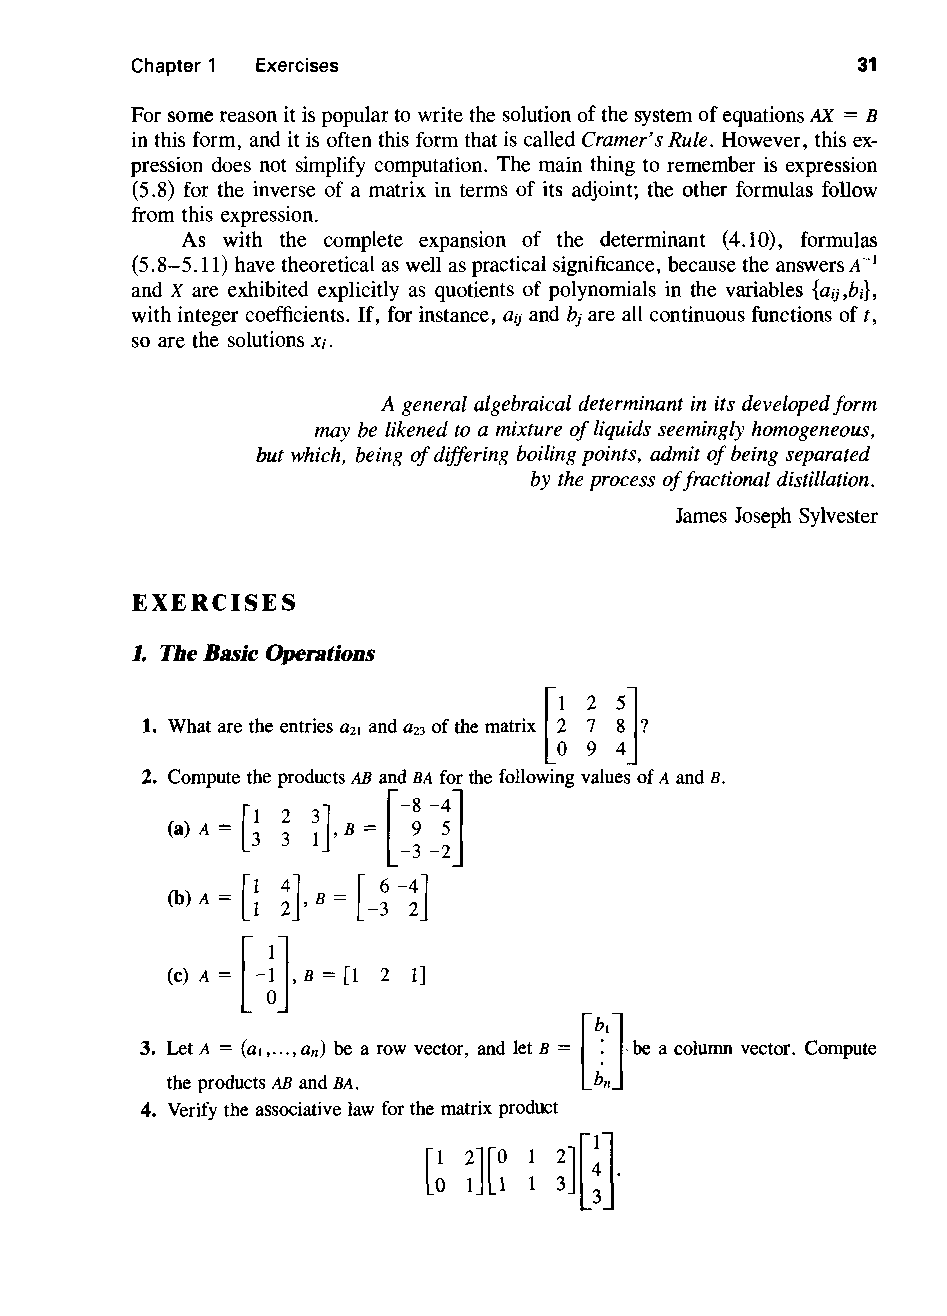
\includepdf[pages={1-},scale=0.85]{Exercises/C1_selection.pdf}
\section{The Basic Operations}
%\section*{Exercises}
\begin{itemize}
\item[(1)]
$a_{21} = 2, s_{23} = 8$
\item[(2)]
\begin{itemize}
\item[(a)]
$$AB = \begin{bmatrix}
1 & 2 & 3 \\
3 & 3 & 1
\end{bmatrix}\begin{bmatrix}
-8 & -4 \\
9 & 5 \\
-3 & -2
\end{bmatrix} = \begin{bmatrix}
1 & 0 \\
0 & 1
\end{bmatrix}$$
$$BA = \begin{bmatrix}
-8 & -4 \\
9 & 5 \\
-3 & -2
\end{bmatrix}\begin{bmatrix}
1 & 2 & 3 \\
3 & 3 & 1
\end{bmatrix} = \begin{bmatrix}
-20 & -28 & - 28 \\
24 & 33 & 33 \\
-9 & -12 & -11
\end{bmatrix}$$
\item[(b)]
$$AB = \begin{bmatrix}
1 & 4 \\
1 & 2
\end{bmatrix}\begin{bmatrix}
6 & -4 \\
-3 & 2
\end{bmatrix} = \begin{bmatrix}
-6 & -4 \\
0 & 0
\end{bmatrix}$$
$$BA = \begin{bmatrix}
6 & -4 \\
-3 & 2
\end{bmatrix}\begin{bmatrix}
1 & 4 \\
1 & 2
\end{bmatrix} = \begin{bmatrix}
2 & 16 \\
-1 & -8
\end{bmatrix}$$
\item[(c)]
$$AB = \begin{bmatrix}
1 \\
-1 \\
0
\end{bmatrix}\begin{bmatrix}
1 & 2 & 1
\end{bmatrix} = \begin{bmatrix}
1 & 2 & 1 \\
-1 & -2 & -1 \\
0 & 0 & 0
\end{bmatrix}$$
$$BA = \begin{bmatrix}
1 & 2 & 1
\end{bmatrix}\begin{bmatrix}
1 \\
-1 \\
0
\end{bmatrix} = \begin{bmatrix}
-1
\end{bmatrix}$$
\end{itemize}
\item[(3)]
$$AB = \begin{bmatrix}
a_1 & \hdots & a_n
\end{bmatrix}\begin{bmatrix}
b_1 \\
\vdots \\
b_n
\end{bmatrix} = \begin{bmatrix}
a_1b_1 + ... + a_nb_n
\end{bmatrix}$$
$$BA = \begin{bmatrix}
b_1 \\
\vdots \\
b_n
\end{bmatrix}\begin{bmatrix}
a_1 & \hdots & a_n
\end{bmatrix} = \begin{bmatrix}
a_1b_1 & a_2b_1 & \hdots & a_nb_1 \\
a_1b_2 & a_2b_2 & \hdots & a_nb_2 \\
\vdots & \vdots & \ddots & \vdots \\
a_1b_n & a_2b_n & \hdots & a_nb_n
\end{bmatrix}$$
\item[(4)]
$$\left( \begin{bmatrix}
1 & 2 \\
0 & 1
\end{bmatrix}\begin{bmatrix}
0 & 1 & 2 \\
1 & 1 & 3
\end{bmatrix} \right)\begin{bmatrix}
1 \\
4 \\
3
\end{bmatrix} = \begin{bmatrix}
2 & 3 & 8 \\
1 & 1 & 3
\end{bmatrix}\begin{bmatrix}
1 \\
4 \\
3
\end{bmatrix} = \begin{bmatrix}
38 \\
14
\end{bmatrix}$$
$$\begin{bmatrix}
1 & 2 \\
0 & 1
\end{bmatrix} \left(\begin{bmatrix}
0 & 1 & 2 \\
1 & 1 & 3
\end{bmatrix}\begin{bmatrix}
1 \\
4 \\
3
\end{bmatrix} \right) = \begin{bmatrix}
1 & 2 \\
0 & 1
\end{bmatrix}\begin{bmatrix}
10 \\
14
\end{bmatrix} = \begin{bmatrix}
38 \\
14
\end{bmatrix}$$
\item[(5)]
$$\begin{bmatrix}
1 & a \\
& 1
\end{bmatrix}\begin{bmatrix}
1 & b \\
& 1
\end{bmatrix} = \begin{bmatrix}
1 & a + b \\
& 1
\end{bmatrix}$$
\item[(6)]
I claim that
$$\begin{bmatrix}
1 & 1 \\
& 1
\end{bmatrix}^n = \begin{bmatrix}
1 & n \\
& 1
\end{bmatrix}$$
Let $n = 1$. Then
$$\begin{bmatrix}
1 & 1 \\
& 1
\end{bmatrix}$$
So the statement is trivially true for $n = 1$. Suppose the statement is true for $n = k - 1$. Then
$$\begin{bmatrix}
1 & 1 \\
& 1
\end{bmatrix}^k = \begin{bmatrix}
1 & 1 \\
& 1
\end{bmatrix}^{k-1}\begin{bmatrix}
1 & 1 \\
& 1
\end{bmatrix} = \begin{bmatrix}
1 & k - 1 \\
& 1
\end{bmatrix}\begin{bmatrix}
1 & 1 \\
& 1
\end{bmatrix} = \begin{bmatrix}
1 & k \\
& 1
\end{bmatrix}$$
\item[(7)]
I claim that
$$\begin{bmatrix}
1 & 1 & 1 \\
& 1 & 1 \\
& & 1
\end{bmatrix}^n = \begin{bmatrix}
1 & n & T_n \\
& 1 & n \\
& & 1
\end{bmatrix}$$
Where $T_n = \sum_{i=1}^n i$

Suppose $n = 1$. Then
$$\begin{bmatrix}
1 & 1 & 1 \\
& 1 & 1 \\
& & 1
\end{bmatrix}^n = \begin{bmatrix}
1 & 1 & 1 \\
& 1 & 1 \\
& & 1
\end{bmatrix}$$
Since $T_1 = 1$, then the statement is true. Suppose the statement is true for $n = k - 1$. Then
$$\begin{bmatrix}
1 & 1 & 1 \\
& 1 & 1 \\
& & 1
\end{bmatrix}^k = \begin{bmatrix}
1 & 1 & 1 \\
& 1 & 1 \\
& & 1
\end{bmatrix}^{k-1}\begin{bmatrix}
1 & 1 & 1 \\
& 1 & 1 \\
& & 1
\end{bmatrix}$$
$$ = \begin{bmatrix}
1 & k-1 & T_{k-1} \\
& 1 & k-1 \\
& & 1
\end{bmatrix}\begin{bmatrix}
1 & 1 & 1 \\
& 1 & 1 \\
& & 1
\end{bmatrix} = \begin{bmatrix}
1 & k-1 + 1 & T_{k-1} + k-1 + 1 \\
& 1 & k -1 + 1 \\
& & 1 
\end{bmatrix}$$
$$= \begin{bmatrix}
1 & k & T_k \\
& 1 & k \\
& & 1
\end{bmatrix}$$
\item[(8)]
$$\begin{bmatrix} 
\begin{array}{cc|cc}
1 & 1 & 1 & 5 \\
0 & 1 & 0 & 1 \\
\hline
1 & 0 & 0 & 1 \\
0 & 1 & 1 & 0
\end{array}
\end{bmatrix}\begin{bmatrix} 
\begin{array}{cc|cc}
1 & 2 & 1 & 0 \\
0 & 1 & 0 & 1 \\
\hline
1 & 0 & 0 & 1 \\
0 & 1 & 1 & 3
\end{array}
\end{bmatrix}$$
$$= \begin{bmatrix}
\begin{array}{c|c}

\begin{bmatrix}
1 & 1 \\
0 & 1
\end{bmatrix} \begin{bmatrix}
1 & 2 \\
0 & 1
\end{bmatrix} + \begin{bmatrix}
1 & 5 \\
0 & 1
\end{bmatrix}\begin{bmatrix}
1 & 0 \\
0 & 1
\end{bmatrix} & \begin{bmatrix}
1 & 1 \\
0 & 1
\end{bmatrix} \begin{bmatrix}
1 & 0 \\
0 & 1
\end{bmatrix} + \begin{bmatrix}
1 & 5 \\
0 & 1
\end{bmatrix}\begin{bmatrix}
0 & 1 \\
1 & 3
\end{bmatrix} \\
\hline
\begin{bmatrix}
1 & 0 \\
0 & 1
\end{bmatrix} \begin{bmatrix}
1 & 2 \\
0 & 1
\end{bmatrix} + \begin{bmatrix}
0 & 1 \\
1 & 0
\end{bmatrix}\begin{bmatrix}
1 & 0 \\
0 & 1
\end{bmatrix} & \begin{bmatrix}
1 & 0 \\
0 & 1
\end{bmatrix} \begin{bmatrix}
1 & 0 \\
0 & 1
\end{bmatrix} + \begin{bmatrix}
0 & 1 \\
1 & 0
\end{bmatrix}\begin{bmatrix}
0 & 1 \\
1 & 3
\end{bmatrix}
\end{array}
\end{bmatrix}$$
$$= \begin{bmatrix}
\begin{array}{c|c}
\begin{bmatrix}
1 & 3 \\
0 & 1
\end{bmatrix} + \begin{bmatrix}
1 & 5 \\
0 & 1
\end{bmatrix} & \begin{bmatrix}
1 & 1 \\
0 & 1
\end{bmatrix} + \begin{bmatrix}
5 & 16 \\
1 & 3
\end{bmatrix} \\
\hline
\begin{bmatrix}
1 & 2 \\
0 & 1
\end{bmatrix} + \begin{bmatrix}
0 & 1 \\
1 & 0
\end{bmatrix} & \begin{bmatrix}
1 & 0 \\
0 & 1
\end{bmatrix} + \begin{bmatrix}
1 & 3 \\
0 & 1
\end{bmatrix}
\end{array}
\end{bmatrix} = \begin{bmatrix}
2 & 8 & 6 & 17 \\
0 & 2 & 1 & 4 \\
1 & 3 & 2 & 3 \\
1 & 1 & 0 & 1
\end{bmatrix}$$
$$\begin{bmatrix} 
\begin{array}{c|cc}
0 & 1 & 2 \\
\hline
0 & 1 & 0 \\
3 & 0 & 1
\end{array}
\end{bmatrix}\begin{bmatrix} 
\begin{array}{c|cc}
1 & 2 & 3 \\
\hline
4 & 2 & 3 \\
5 & 0 & 4
\end{array}
\end{bmatrix}$$
$$= \begin{bmatrix} 
\begin{array}{c|c}
\begin{bmatrix}
0
\end{bmatrix}\begin{bmatrix}
1
\end{bmatrix} + \begin{bmatrix}
1 & 2
\end{bmatrix}\begin{bmatrix}
4 \\
5
\end{bmatrix} & \begin{bmatrix}
0
\end{bmatrix}\begin{bmatrix}
2 & 3
\end{bmatrix} + \begin{bmatrix}
1 & 2
\end{bmatrix}\begin{bmatrix}
2 & 3 \\
0 & 4
\end{bmatrix} \\
\hline
\begin{bmatrix}
0 \\
3
\end{bmatrix}\begin{bmatrix}
1
\end{bmatrix} + \begin{bmatrix}
1 & 0 \\
0 & 1
\end{bmatrix}\begin{bmatrix}
4 \\
5
\end{bmatrix} & \begin{bmatrix}
0 \\
3
\end{bmatrix}\begin{bmatrix}
2 & 3
\end{bmatrix} + \begin{bmatrix}
1 & 0 \\
0 & 1
\end{bmatrix}\begin{bmatrix}
2 & 3 \\
0 & 4
\end{bmatrix}
\end{array}
\end{bmatrix}$$
$$= \begin{bmatrix}
\begin{array}{c|c}
\begin{bmatrix}
0
\end{bmatrix} + \begin{bmatrix}
14
\end{bmatrix} & \begin{bmatrix}
0 & 0
\end{bmatrix} + \begin{bmatrix}
2 & 11
\end{bmatrix} \\
\hline
\begin{bmatrix}
0 \\
3
\end{bmatrix} + \begin{bmatrix}
4 \\
5
\end{bmatrix} & \begin{bmatrix}
0 & 0 \\
6 & 9
\end{bmatrix} + \begin{bmatrix}
2 & 3 \\
0 & 4
\end{bmatrix}
\end{array}
\end{bmatrix} = \begin{bmatrix}
14 & 2 & 11 \\
4 & 2 & 3 \\
8 & 6 & 13
\end{bmatrix}$$
\item[(9)]
Let $M$ be a $m \times n$ matrix and $M'$ be a $n \times p$ matrix where 
$$M = \begin{bmatrix}
\begin{array}{c|c}
A & B \\
\hline
C & D
\end{array}
\end{bmatrix} = \begin{bmatrix}
\begin{array}{cccc|cccc}
a_{11} & a_{12} & \hdots & a_{1i} & b_{11} & b_{12} & \hdots & b_{1 n-i} \\
a_{21} & a_{22} & \hdots & a_{2i} & b_{21} & b_{22} & \hdots & b_{2 n-i} \\
\vdots & \vdots & \ddots & \vdots & \vdots & \vdots & \ddots & \vdots \\
a_{j1} & a_{j2} & \hdots & a_{ji} & b_{j1} & b_{j2} & \hdots & b_{j n-i} \\
\hline
c_{11} & c_{12} & \hdots & c_{1i} & d_{11} & d_{12} & \hdots & d_{1 n-i} \\
c_{21} & c_{22} & \hdots & c_{2i} & d_{21} & d_{22} & \hdots & d_{2 n-i} \\
\vdots & \vdots & \ddots & \vdots & \vdots & \vdots & \ddots & \vdots \\
c_{m-j 1} & c_{m-j 2} & \hdots & c_{m-j i} & d_{m-j 1} & d_{m-j 2} & \hdots & d_{m-j n-i} \\
\end{array}
\end{bmatrix}$$
$$M' = \begin{bmatrix}
\begin{array}{c|c}
A' & B' \\
\hline
C' & D'
\end{array}
\end{bmatrix} = \begin{bmatrix}
\begin{array}{cccc|cccc}
a'_{11} & a'_{12} & \hdots & a'_{1x} & b'_{11} & b'_{12} & \hdots & b'_{1 p-x} \\
a'_{21} & a'_{22} & \hdots & a'_{2x} & b'_{21} & b'_{22} & \hdots & b'_{2 p-x} \\
\vdots & \vdots & \ddots & \vdots & \vdots & \vdots & \ddots & \vdots \\
a'_{i1} & a'_{i2} & \hdots & a'_{ix} & b'_{i1} & b'_{i2} & \hdots & b'_{i p-x} \\
\hline
c'_{11} & c'_{12} & \hdots & c'_{1x} & d'_{11} & d'_{12} & \hdots & d'_{1 p-x} \\
c'_{21} & c'_{22} & \hdots & c'_{2x} & d'_{21} & d'_{22} & \hdots & d'_{2 p-x} \\
\vdots & \vdots & \ddots & \vdots & \vdots & \vdots & \ddots & \vdots \\
c'_{n-i 1} & c'_{n-i 2} & \hdots & c'_{n-i x} & d'_{n-i 1} & d'_{n-i 2} & \hdots & d'_{n-i p-x} \\
\end{array}
\end{bmatrix}$$
Then
$$MM' = \begin{bmatrix}
\sum_{k=1}^i a_{1k}a'_{k1} + \sum_{k=1}^{n-i} b_{1k}c'_{k1} & \hdots & \sum_{k=1}^i a_{1k}b'_{k p-x} + \sum_{k=1}^{n-i} b_{1k}d'_{k p-x} \\
\vdots & \ddots & \vdots \\
 \sum_{k=1}^i c_{1k}a'_{k1} + \sum_{k=1}^{n-i} d_{1k}c'_{k1} & \hdots & \sum_{k=1}^i c_{1k}b'_{k p-x} + \sum_{k=1}^{n-i} d_{1k}d'_{k p-x}
\end{bmatrix}$$
$$= \begin{bmatrix}
\begin{array}{c|c}
AA' + AC' & A'B + BD' \\
\hline
CA' + DC' & CB' + DD'
\end{array}
\end{bmatrix}$$
\item[(10)]
\begin{itemize}
\item[(a)]
$$A^2 - B^2 = (A + B)(A - B) = A^2 + BA - AB - B^2 \rightarrow BA = AB$$
\item[(b)]
$$(A + B)^3 = (A + B)(A^2 + AB + BA + B^2)$$
$$= A^3 + A^2B + ABA + AB^2 + BA^2 + BAB + B^2A + B^3$$
\end{itemize}
\item[(11)]
\begin{itemize}
\item[(a)]
$$DA = \begin{bmatrix}
d_1a_{11} & d_1a_{12} & \hdots & d_1a_{1n} \\
d_2a_{21}& d_2a_{22} & \hdots & d_2a_{2n} \\
\vdots & \vdots & \ddots & \vdots \\
d_na_{n1} & d_na_{n2} & \vdots & d_na_{nn}
\end{bmatrix}$$
$$AD = \begin{bmatrix}
d_1a_{11} & d_2a_{12} & \hdots & d_na_{1n} \\
d_1a_{21} & d_2a_{22} & \hdots & d_na_{2n} \\
\vdots & \vdots & \ddots & \vdots \\
d_1a_{n1} & d_2a_{n2} & \hdots & d_na_{nn}
\end{bmatrix}$$
\item[(b)]
Let $D, D'$ be $n \times n$ diagonal matrices with entries $d_{ii}$ and $d'_{ii}$ respectively. Then
$$DD' = \begin{bmatrix}
d_{11}d'_{11} & & & \\
& d_{22}d'_{22} & & \\
& & \ddots & \\
& & & d_{nn}d'_{nn}
\end{bmatrix}$$
\item[(c)]
From part (a), each diagonal entry $i$ of either product $DA$ or $AD$ equals $d_ia_{ii}$. If $A$ is an inverse of $D$, then each $d_ia_{ii} = 1$, implying each diagonal entry of $D$ must be nonzero.
\end{itemize}
\item[(12)]
Let $A, B$ be $n \times n$ upper triangular matrices. Then
$$(AB)_{ij} = \sum_{k=1}^n a_{ik}b_{kj} = \sum_{k=i}^j a_{ik}b_{kj}$$
Since $i > j$, then $(AB)_{ij} = 0$. Therefore, $AB$ is upper triangular.
\item[(13)]
\begin{itemize}
\item[(a)]
$$\begin{bmatrix}
1 & 0 \\
0 & 0
\end{bmatrix}\begin{bmatrix}
a & b \\
c & d
\end{bmatrix} = \begin{bmatrix}
a & b \\
c & d
\end{bmatrix}\begin{bmatrix}
1 & 0 \\
0 & 0
\end{bmatrix}$$
$$\rightarrow \begin{bmatrix}
a & b \\
0 & 0
\end{bmatrix} = \begin{bmatrix}
a & 0 \\
c & 0
\end{bmatrix}$$
Thus, a matrix that commutes has the form
$$\begin{bmatrix}
a & 0 \\
0 & 0
\end{bmatrix}$$
\item[(b)]
$$\begin{bmatrix}
0 & 1 \\
0 & 0
\end{bmatrix}\begin{bmatrix}
a & b \\
c & d
\end{bmatrix} = \begin{bmatrix}
a & b \\
c & d
\end{bmatrix}\begin{bmatrix}
0 & 1 \\
0 & 0
\end{bmatrix}$$
$$\rightarrow \begin{bmatrix}
c & d \\
0 & 0
\end{bmatrix} = \begin{bmatrix}
0 & a \\
0 & c
\end{bmatrix}$$
Thus, a matrix that commutes has the form
$$\begin{bmatrix}
0 & a \\
0 & 0
\end{bmatrix}$$
\item[(c)]
$$\begin{bmatrix}
2 & 0 \\
0 & 6
\end{bmatrix}\begin{bmatrix}
a & b \\
c & d
\end{bmatrix} = \begin{bmatrix}
a & b \\
c & d
\end{bmatrix}\begin{bmatrix}
2 & 0 \\
0 & 6
\end{bmatrix}$$
$$\rightarrow \begin{bmatrix}
2a & 2b \\
6c & 6d
\end{bmatrix} = \begin{bmatrix}
2a & 6b \\
2c & 6d
\end{bmatrix}$$
Thus, a matrix that commutes has the form
$$\begin{bmatrix}
a & 0 \\
0 & d
\end{bmatrix}$$
\item[(d)]
$$\begin{bmatrix}
1 & 3 \\
0 & 1
\end{bmatrix}\begin{bmatrix}
a & b \\
c & d
\end{bmatrix} = \begin{bmatrix}
a & b \\
c & d
\end{bmatrix}\begin{bmatrix}
1 & 3 \\
0 & 1
\end{bmatrix}$$
$$\rightarrow \begin{bmatrix}
a + 3c & b + 3d \\
c & d
\end{bmatrix} = \begin{bmatrix}
a & 3a + b \\
c & 3c + d
\end{bmatrix}$$
Thus, a matrix that commutes has the form
$$\begin{bmatrix}
a & b \\
0 & a
\end{bmatrix}$$
\item[(e)]
$$\begin{bmatrix}
2 & 3 \\
0 & 6
\end{bmatrix}\begin{bmatrix}
a & b \\
c & d
\end{bmatrix} = \begin{bmatrix}
a & b \\
c & d
\end{bmatrix}\begin{bmatrix}
2 & 3 \\
0 & 6
\end{bmatrix}$$
$$\rightarrow \begin{bmatrix}
2a + 3c & 2b + 3d \\
6c & 6d
\end{bmatrix} = \begin{bmatrix}
2a & 3a + 6b \\
2c & 3c + 6d
\end{bmatrix}$$
Thus, a matrix that commutes has the form
$$\begin{bmatrix}
a & \frac{3}{4}(d - a) \\
0 & d
\end{bmatrix}$$
\end{itemize}
\item[(14)]
Let $A = (a_{ij})$ be an $n \times n$ matrix. Then
$$0 + A = \begin{bmatrix}
0 & \hdots & 0 \\
\vdots & \ddots & \vdots \\
0 & \hdots & 0
\end{bmatrix} + \begin{bmatrix}
a_{11} & \hdots & a_{1n} \\
\vdots & \ddots & \vdots \\
a_{n1} & \hdots & a_{nn}
\end{bmatrix}$$
$$= \begin{bmatrix}
0 + a_{11} & \hdots & 0 + a_{1n} \\
\vdots & \ddots & \vdots \\
0 + a_{n1} & \hdots & 0 + a_{nn}
\end{bmatrix} = \begin{bmatrix}
a_{11} & \hdots & a_{1n} \\
\vdots & \ddots & \vdots \\
a_{n1} & \hdots & a_{nn}
\end{bmatrix} = A$$
$$0A = \begin{bmatrix}
0 & \hdots & 0 \\
\vdots & \ddots & \vdots \\
0 & \hdots & 0
\end{bmatrix}\begin{bmatrix}
a_{11} & \hdots & a_{1n} \\
\vdots & \ddots & \vdots \\
a_{n1} & \hdots & a_{nn}
\end{bmatrix}$$
$$ = \begin{bmatrix}
0a_{11} + \hdots + 0a_{n1} & \hdots & 0a_{1n} + \hdots + 0a_{nn} \\
\vdots & \ddots & \vdots \\
0a_{11} + \hdots + 0a_{n1} & \hdots & 0a_{1n} + \hdots + 0a_{nn}
\end{bmatrix} = \begin{bmatrix}
0 & \hdots & 0 \\
\vdots & \ddots & \vdots \\
0 & \hdots & 0
\end{bmatrix} = 0$$
$$A0 = \begin{bmatrix}
a_{11} & \hdots & a_{1n} \\
\vdots & \ddots & \vdots \\
a_{n1} & \hdots & a_{nn}
\end{bmatrix}\begin{bmatrix}
0 & \hdots & 0 \\
\vdots & \ddots & \vdots \\
0 & \hdots & 0
\end{bmatrix}$$
$$= \begin{bmatrix}
0a_{11} + \hdots + 0a_{1n} & \hdots & 0a_{11} + \hdots + 0a_{1n} \\
\vdots & \ddots & \vdots \\
0a_{n1} + \hdots + 0a_{nn} & \hdots & 0a_{n1} + \hdots + 0a_{nn}
\end{bmatrix} = \begin{bmatrix}
0 & \hdots & 0 \\
\vdots & \ddots & \vdots \\
0 & \hdots & 0
\end{bmatrix} = 0$$
\item[(15)]
Suppose an $n \times n$ $A$ matrix has a row $i$ of zeros. Then for any $n \times n$ matrix $B$,
$$(AB)_{ii} = \sum_{k=1}^n a_{ik}b_{ki} = 0$$
So $B$ cannot be an inverse of $A$, so $A$ is not invertible.
\item[(16)]
Suppose $k = 1$. Then $A = 0$, so trivially $I + A = I$ is invertible: its inverse is $I$.

Suppose $k > 1$. Consider $B = I + \sum_{i=1}^{k-1}(-1)^iA^i$. Then
$$(I+A)B = I + \sum_{i=1}^{k-1}\left((-1)^iA^i + (-1)^iA^{i+1}\right)$$
$$= I + (-1)^kA^k + \sum_{i=1}^{k-1}
\left( (-1)^{i-1}A^i + (-1)^iA^i \right) = I$$
Furthermore,
$$B(I+A) = I + \sum_{i=1}^{k-1}\left((-1)^iA^i + (-1)^iA^{i+1}\right)$$
$$= I + (-1)^kA^k + \sum_{i=1}^{k-1}
\left( (-1)^{i-1}A^i + (-1)^iA^i \right) = I$$
Thus, $(I + A)^{-1} = B$
\item[(17)]
\begin{itemize}
\item[(a)]
Consider the $2 \times 3$ matrix $B$ that is a left inverse of $A$, where
$$B = \begin{bmatrix}
a & b & c \\
d & e & f
\end{bmatrix}$$
Then
$$BA = \begin{bmatrix}
a & b & c \\
d & e & f
\end{bmatrix}\begin{bmatrix}
2 & 3 \\
1 & 2 \\
2 & 5
\end{bmatrix}$$
$$= \begin{bmatrix}
2a + b + 2c & 3a + 2b + 5c \\
2d + e + 2f & 3d + 2e + 5f
\end{bmatrix} = \begin{bmatrix}
1 & 0 \\
0 & 1
\end{bmatrix}$$
Thus
$$B = \begin{bmatrix}
2 + c & -3 - 4c & c \\
f - 1 & 2 - 4f & f
\end{bmatrix}$$
\item[(b)]
Consider the $2 \times 3$ matrix $C$, where
$$C = \begin{bmatrix}
a & b & c \\
d & e & f
\end{bmatrix}$$
Suppose $C$ is a right inverse of $A$. Then
$$AC = \begin{bmatrix}
2 & 3 \\
1 & 2 \\
2 & 5
\end{bmatrix}\begin{bmatrix}
a & b & c \\
d & e & f
\end{bmatrix}$$
$$ = \begin{bmatrix}
2a + 3d & 2b + 3e & 2c + 3f \\
a + 2d & b + 2e & c + 2f \\
2a + 5d & 2a + 5e & 2a + 5f
\end{bmatrix} = \begin{bmatrix}
1 & & \\
& 1 & \\
& & 1
\end{bmatrix} $$
In particular, $a + 2d = 2a + 5d = 0$ implies that $a = 0$ and $d = 0$. But then $0 = 2a + 3d = 1$, a contradiction. Thus $C$ cannot be a right inverse of $A$.
\end{itemize}
\item[(18)]
Assume $A, B$ are invertible. We can then check if $B^{-1}A^{-1}$ is the inverse of $AB$:
$$(AB)(B^{-1}A^{-1}) = A(BB^{-1})A^{-1} = A(I)A^{-1} = AA^{-1} = I$$
Similarly,
$$(B^{-1}A^{-1})(AB) = B^{-1}(A^{-1}A)B = B^{-1}(I)B = B^{-1}B = I$$
\item[(19)]
\begin{itemize}
\item[(a)]
Let $C = A + B$. Then $c_{ij} = a_{ij} + b_{ij}$. So
$$\text{tr }C = \sum_{i=1}^n c_{ii} = \sum_{i=1}^n a_{ii} + \sum_{i=1}^n b_{ii} = \text{tr }A + \text{tr }B$$
Let $D = AB$ and $E = BA$. Then $d_{ij} = \sum_{k=1}^n a_{ik}b_{kj}$, and $e_{ij} = \sum_{k=1}^n b_{ik}a_{kj}$. So
$$\text{tr }D = \sum_{i = 1}^n d_{ii} = \sum_{i=1}^n\sum_{k=1}^n a_{ik}b_{ki} = \sum_{k=1}^n\sum_{i=1}^n b_{ki}a_{ik} = \sum_{k=1}^n e_{kk} = \text{tr }E$$
\item[(b)]
Let $C = BA$. Then
$$\text{tr }BAB^{-1} = \text{tr }CB^{-1} \text{tr }B^{-1}C = \text{tr }B^{-1}BA = \text{tr }A$$
\end{itemize}
\item[(20)]
Note that $\text{tr }I = n$. Furthermore, for any matrix $A$ and a constant $c$, 
$$\text{tr }cA = ca_{11} + ca_{22} + ... + ca_{nn} = c(a_{11} + a_{22} + ... + a_{nn}) = c \cdot \text{tr }A$$ 
But
$$\text{tr }(AB - BA) = \text{tr }AB + \text{tr }(-1)BA = \text{tr }AB - \text{tr }BA = 0$$
Therefore, $AB - BA \neq I$.
\end{itemize}

\section{Row Reduction}
\begin{itemize}
\item[(1)]
\begin{itemize}
\item[(a)]
$$E_1 = \begin{bmatrix}
1 & 0 & 0 \\
-1 & 1 & 0 \\
0 & 0 & 1
\end{bmatrix}, E_2 = \begin{bmatrix}
1 & 0 & 0 \\
0 & 1 & 0 \\
-1 & 0 & 1
\end{bmatrix}, E_3 = \begin{bmatrix}
1 & 0 & 0 \\
0 & 1 & 0 \\
0 & -2 & 1
\end{bmatrix}$$
$$E_4 = \begin{bmatrix}
1 & 0 & 0 \\
0 & 1 & -1 \\
0 & 0 & 1
\end{bmatrix}, E_5 = \begin{bmatrix}
1 & 0 & -1 \\
0 & 1 & 0 \\
0 & 0 & 1
\end{bmatrix}$$
\item[(b)]
$$P = E_5E_4E_3E_2E_1$$
$$= \begin{bmatrix}
1 & 0 & -1 \\
0 & 1 & 0 \\
0 & 0 & 1
\end{bmatrix}\begin{bmatrix}
1 & 0 & 0 \\
0 & 1 & -1 \\
0 & 0 & 1
\end{bmatrix}\begin{bmatrix}
1 & 0 & 0 \\
0 & 1 & 0 \\
0 & -2 & 1
\end{bmatrix}\begin{bmatrix}
1 & 0 & 0 \\
0 & 1 & 0 \\
-1 & 0 & 1
\end{bmatrix}\begin{bmatrix}
1 & 0 & 0 \\
-1 & 1 & 0 \\
0 & 0 & 1
\end{bmatrix}$$
$$= \begin{bmatrix}
1 & 0 & -1 \\
0 & 1 & 0 \\
0 & 0 & 1
\end{bmatrix}\begin{bmatrix}
1 & 0 & 0 \\
0 & 1 & -1 \\
0 & 0 & 1
\end{bmatrix}\begin{bmatrix}
1 & 0 & 0 \\
0 & 1 & 0 \\
0 & -2 & 1
\end{bmatrix}\begin{bmatrix}
1 & 0 & 0 \\
-1 & 1 & 0 \\
-1 & 0 & 1
\end{bmatrix}$$
$$= \begin{bmatrix}
1 & 0 & -1 \\
0 & 1 & 0 \\
0 & 0 & 1
\end{bmatrix}\begin{bmatrix}
1 & 0 & 0 \\
0 & 1 & -1 \\
0 & 0 & 1
\end{bmatrix}\begin{bmatrix}
1 & 0 & 0 \\
-1 & 1 & 0 \\
1 & -2 & 1
\end{bmatrix}$$
$$= \begin{bmatrix}
1 & 0 & -1 \\
0 & 1 & 0 \\
0 & 0 & 1
\end{bmatrix}\begin{bmatrix}
1 & 0 & 0 \\
-2 & 3 & -1 \\
1 & -2 & 1
\end{bmatrix} = \begin{bmatrix}
0 & 2 & -1 \\
-2 & 3 & -1 \\
1 & -2 & 1
\end{bmatrix}$$
$$PM = \begin{bmatrix}
0 & 2 & -1 \\
-2 & 3 & -1 \\
1 & -2 & 1
\end{bmatrix}\begin{bmatrix}
1 & 0 & 2 & 1 & 5 \\
1 & 1 & 5 & 2 & 7 \\
1 & 2 & 8 & 4 & 12
\end{bmatrix} = \begin{bmatrix}
1 & 0 & 2 & 0 & 2 \\
0 & 1 & 3 & 0 & -1 \\
0 & 0 & 0 & 1 & 3
\end{bmatrix}$$
\end{itemize}
\item[(2)]
\begin{itemize}
\item[(a)]
$$\begin{bmatrix}
\begin{array}{cccc|c}
1 & 2 & 1 & 1 & 0 \\
3 & 0 & 0 & 4 & 0 \\
1 & -4 & -2 & -2 & 0
\end{array}
\end{bmatrix} \rightarrow\rightarrow \begin{bmatrix}
\begin{array}{cccc|c}
1 & 2 & 1 & 1 & 0 \\
0 & -6 & -3 & 1 & 0 \\
0 & -6 & -3 & -3 & 0
\end{array}
\end{bmatrix}$$
$$ \rightarrow \begin{bmatrix}
\begin{array}{cccc|c}
1 & 2 & 1 & 1 & 0 \\
0 & 1 & 1/2 & -1/6 & 0 \\
0 & -6 & -3 & -3 & 0
\end{array}
\end{bmatrix} \rightarrow \begin{bmatrix}
\begin{array}{cccc|c}
1 & 2 & 1 & 1 & 0 \\
0 & 1 & 1/2 & -1/6 & 0 \\
0 & 0 & 0 & -4 & 0
\end{array}
\end{bmatrix}$$
$$\rightarrow \begin{bmatrix}
\begin{array}{cccc|c}
1 & 2 & 1 & 1 & 0 \\
0 & 1 & 1/2 & -1/6 & 0 \\
0 & 0 & 0 & 1 & 0
\end{array}
\end{bmatrix}\rightarrow\rightarrow \begin{bmatrix}
\begin{array}{cccc|c}
1 & 2 & 1 & 0 & 0 \\
0 & 1 & 1/2 & 0 & 0 \\
0 & 0 & 0 & 1 & 0
\end{array}
\end{bmatrix}$$
$$\rightarrow \begin{bmatrix}
\begin{array}{cccc|c}
1 & 0 & 0 & 0 & 0 \\
0 & 1 & 1/2 & 0 & 0 \\
0 & 0 & 0 & 1 & 0
\end{array}
\end{bmatrix}$$
For arbitrary $x_3$, then $x_4 = 0, x_2 = -x_3/2, x_1 = 0$.
\item[(b)]
$$\begin{bmatrix}
\begin{array}{cccc|c}
1 & 2 & 1 & 1 & 1 \\
3 & 0 & 0 & 4 & 1 \\
1 & -4 & -2 & -2 & 0
\end{array}
\end{bmatrix} \rightarrow\rightarrow \begin{bmatrix}
\begin{array}{cccc|c}
1 & 2 & 1 & 1 & 1 \\
0 & -6 & -3 & 1 & -2 \\
0 & -6 & -3 & -3 & -1
\end{array}
\end{bmatrix}$$
$$ \rightarrow \begin{bmatrix}
\begin{array}{cccc|c}
1 & 2 & 1 & 1 & 1 \\
0 & 1 & 1/2 & -1/6 & 1/3 \\
0 & -6 & -3 & -3 & -1
\end{array}
\end{bmatrix} \rightarrow \begin{bmatrix}
\begin{array}{cccc|c}
1 & 2 & 1 & 1 & 1 \\
0 & 1 & 1/2 & -1/6 & 1/3 \\
0 & 0 & 0 & -4 & 1
\end{array}
\end{bmatrix}$$
$$\rightarrow \begin{bmatrix}
\begin{array}{cccc|c}
1 & 2 & 1 & 1 & 1 \\
0 & 1 & 1/2 & -1/6 & 1/3 \\
0 & 0 & 0 & 1 & -1/4
\end{array}
\end{bmatrix}\rightarrow\rightarrow \begin{bmatrix}
\begin{array}{cccc|c}
1 & 2 & 1 & 0 & 5/4 \\
0 & 1 & 1/2 & 0 & 7/24 \\
0 & 0 & 0 & 1 & -1/4
\end{array}
\end{bmatrix}$$
$$\rightarrow \begin{bmatrix}
\begin{array}{cccc|c}
1 & 0 & 0 & 0 & 1/2 \\
0 & 1 & 1/2 & 0 & 7/24 \\
0 & 0 & 0 & 1 & -1/4
\end{array}
\end{bmatrix}$$
For arbitrary $x_3$, $x_4 = -1/4$, $x_2 = 7/24 - x_3/2, x_1 = 2/3$.
\item[(c)]
$$\begin{bmatrix}
\begin{array}{cccc|c}
1 & 2 & 1 & 1 & 0 \\
3 & 0 & 0 & 4 & 2 \\
1 & -4 & -2 & -2 & 2
\end{array}
\end{bmatrix} \rightarrow\rightarrow \begin{bmatrix}
\begin{array}{cccc|c}
1 & 2 & 1 & 1 & 0 \\
0 & -6 & -3 & 1 & 2 \\
0 & -6 & -3 & -3 & 2
\end{array}
\end{bmatrix}$$
$$ \rightarrow \begin{bmatrix}
\begin{array}{cccc|c}
1 & 2 & 1 & 1 & 0 \\
0 & 1 & 1/2 & -1/6 & -1/3 \\
0 & -6 & -3 & -3 & 2
\end{array}
\end{bmatrix} \rightarrow \begin{bmatrix}
\begin{array}{cccc|c}
1 & 2 & 1 & 1 & 0 \\
0 & 1 & 1/2 & -1/6 & -1/3 \\
0 & 0 & 0 & -4 & 0
\end{array}
\end{bmatrix}$$
$$\rightarrow \begin{bmatrix}
\begin{array}{cccc|c}
1 & 2 & 1 & 1 & 0 \\
0 & 1 & 1/2 & -1/6 & -1/3 \\
0 & 0 & 0 & 1 & 0
\end{array}
\end{bmatrix}\rightarrow\rightarrow \begin{bmatrix}
\begin{array}{cccc|c}
1 & 2 & 1 & 0 & 0 \\
0 & 1 & 1/2 & 0 & -1/3 \\
0 & 0 & 0 & 1 & 0
\end{array}
\end{bmatrix}$$
$$\rightarrow \begin{bmatrix}
\begin{array}{cccc|c}
1 & 0 & 0 & 0 & 2/3 \\
0 & 1 & 1/2 & 0 & -1/3 \\
0 & 0 & 0 & 1 & 0
\end{array}
\end{bmatrix}$$
For arbitrary $x_3$, $x_4 = 0$, $x_2 = -1/3 - x_3/2, x_1 = 2/3$.
\end{itemize}
\item[(3)]
For arbitrary $x_2, x_3, x_4$, $x_1 = 3 - x_2 - 2x_3 + x_4$
\item[(4)]
$$E_1 = \begin{bmatrix}
1 & 0 \\
-1 & 1
\end{bmatrix}, E_2 = \begin{bmatrix}
1 & -4 \\
0 & 1
\end{bmatrix}, E_3 = \begin{bmatrix}
1 & 0 \\
-1 & 1
\end{bmatrix}$$
$$A^{-1} = E_3E_2E_1 = \begin{bmatrix}
1 & 0 \\
-1 & 1
\end{bmatrix}\begin{bmatrix}
1 & -4 \\
0 & 1
\end{bmatrix}\begin{bmatrix}
1 & 0 \\
-1 & 1
\end{bmatrix}$$
$$= \begin{bmatrix}
1 & 0 \\
-1 & 1
\end{bmatrix}\begin{bmatrix}
5 & -4 \\
-1 & 1
\end{bmatrix} = \begin{bmatrix}
5 & -4 \\
-6 & 5
\end{bmatrix}$$
\item[(5)]
$$A = \begin{bmatrix}
1 & \\
& 2
\end{bmatrix} \rightarrow \begin{bmatrix}
1 & \\
& 1
\end{bmatrix} \Rightarrow A^{-1} = \begin{bmatrix}
1 & \\
& 1/2
\end{bmatrix} $$
$$B = \begin{bmatrix}
1 & 1 \\
& 1
\end{bmatrix} \rightarrow \begin{bmatrix}
1 & \\
& 1
\end{bmatrix} \Rightarrow B^{-1} = \begin{bmatrix}
1 & -1 \\
& 1
\end{bmatrix}$$
$$C = \begin{bmatrix}
& 1 \\
1 &
\end{bmatrix} \rightarrow \begin{bmatrix}
& 1 \\
1 &
\end{bmatrix} \Rightarrow C^{-1} = \begin{bmatrix}
& 1 \\
1 &
\end{bmatrix}$$
$$D = \begin{bmatrix}
3 & 5 \\
1 & 2
\end{bmatrix} \rightarrow \begin{bmatrix}
1 & 5/3 \\
1 & 2
\end{bmatrix} \rightarrow \begin{bmatrix}
1 & 5/3 \\
& 1/3
\end{bmatrix} \rightarrow \begin{bmatrix}
1 & 5/3 \\
& 1
\end{bmatrix} \rightarrow \begin{bmatrix}
1 & \\
& 1
\end{bmatrix}$$
$$D^{-1} = \begin{bmatrix}
1 & -5/3 \\
& 1
\end{bmatrix}\begin{bmatrix}
1 & \\
& 3
\end{bmatrix}\begin{bmatrix}
1 & \\
-1 & 1
\end{bmatrix}\begin{bmatrix}
1/3 & \\
& 1
\end{bmatrix}$$
$$= \begin{bmatrix}
1 & -5/3 \\
& 1
\end{bmatrix}\begin{bmatrix}
1 & \\
& 3
\end{bmatrix}\begin{bmatrix}
1/3 & \\
-1/3 & 1
\end{bmatrix} = \begin{bmatrix}
1 & -5/3 \\
& 1
\end{bmatrix}\begin{bmatrix}
1/3 & \\
-1 & 3
\end{bmatrix}$$
$$= \begin{bmatrix}
2 & -5 \\
-1 & 3
\end{bmatrix}$$
$$E = \begin{bmatrix}
1 & 1 \\
& 1
\end{bmatrix}\begin{bmatrix}
& 1 \\
1 &
\end{bmatrix}\begin{bmatrix}
3 & 5 \\
1 & 2
\end{bmatrix} = BCD$$
$$(BCD)^{-1} = D^{-1}C^{-1}B^{-1} = \begin{bmatrix}
2 & -5 \\
-1 & 3
\end{bmatrix}\begin{bmatrix}
& 1 \\
1 &
\end{bmatrix}\begin{bmatrix}
1 & -1 \\
& 1
\end{bmatrix}$$
$$= \begin{bmatrix}
2 & -5 \\
-1 & 3
\end{bmatrix}\begin{bmatrix}
& 1 \\
1 & -1
\end{bmatrix} = \begin{bmatrix}
-5 & 7 \\
3 & -4
\end{bmatrix}$$
\item[(6)]
$Ae_1 = \begin{bmatrix}
2 & 2
\end{bmatrix}^\top, Ae_2 = \begin{bmatrix}
-1 & 3
\end{bmatrix}^\top$

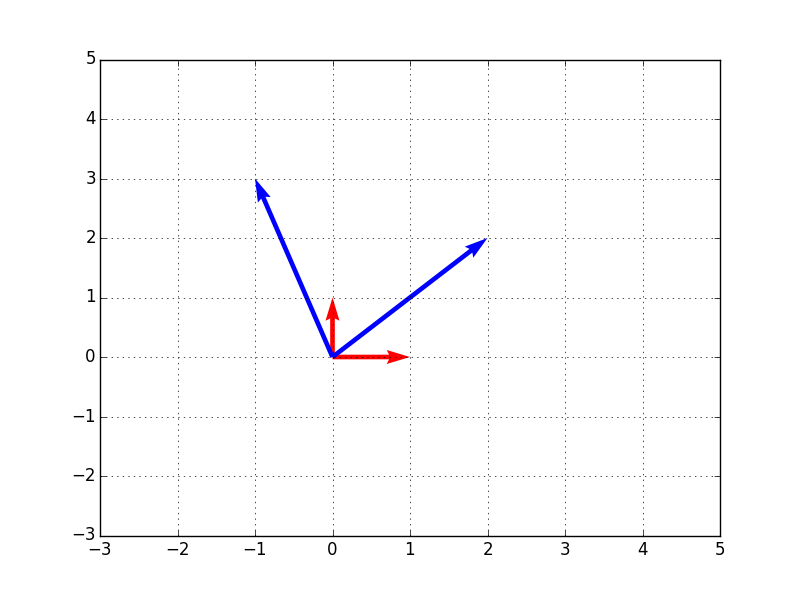
\includegraphics[scale=0.5]{fig/C1_S2_6.png}
\item[(7)]
Suppose we have a matrix $A$ in row reduced echelon form:
$$A = \begin{bmatrix}
\begin{array}{c|c|c}
& 1 & B \\
\hline
& & D
\end{array}
\end{bmatrix}$$
Suppose we can inductively reduce the submatrix $D$ with column operations such that all pivots are denoted with a 1, and all other values are 0. Then we use column operations to negate out all values in $B$. Thus, $A$ can be reduced to a matrix which only has 1's in the locations of the pivots, and all other values are 0.
\item[(8)]
\begin{itemize}
\item[(a)]
Let $A = e_{ij}$, $B = e_{k\ell}$, $E = AB$. Then
$$E_{xy} = \sum_{z = 1}^n A_{xz}B_{zy}$$
Note that if $j=k$, then
$$E_{i\ell} = \sum_{z=1}^n A_{iz}B_{z\ell} = A_{ij}B_{k\ell} = 1$$
If $j \neq k$, then $E_{i\ell} = 0$. For all other $x, y$, then $E_{xy} = 0$. 
\item[(b)]
$$I = e_{11} + e_{22} + ... + e_{nn} = \sum_{i=1}^n e_{ii}$$
\item[(c)]
Denote $A^{(k)}$ the $n \times n$ matrix where for each $i$, $A^{(k)}_{ik} = A_{ik}$, and $A^{(k)}_{ij} = A_{ij}$ for $j \neq k$. Then
$$e_{ii}Ae_{jj} = e_{ii}A^{(j)} = A_{ij}e_{ii}$$
\item[(d)]
Denote $B = e_{ij}A$. If $a = i$, then for all $b$, $B_{ab} = A_{jb}$. Otherwise, $B_{ab} = 0$.

Denote $C = Ae_{ij}$. If $b = j$, then for all $a$, $C_{ab} = A_{ai}$. Otherwise, $C_{ab} = 0$.
\end{itemize}
\item[(9)]
Let $X$ be an arbitrary matrix. Let $E_1 = I + ae_{ij}$ be a type (i) matrix. Then
$$E_1X = (I + ae_{ij}X) = X + ae_{ij}X$$
Then, if $x = i$, then for all $y$, $(E_1X)_{xy} = X_{iy} + aX_{jy}$, ie. scaling row $j$ by a and adding it to row $i$. If $x \neq i$, then for all $y$, $(E_1X)_{xy} = X_{xy}$.

Let $E_2 = I + e_{ij} + e_{ji} - e_{ii} - e_{jj}$ be a type (ii) matrix. Then
$$E_2X = (I + e_{ij} + e_{ji} - e_{ii} - e_{jj})X = X + e_{ij}X + e_{ji}X - e_{ii}X - e_{jj}X$$
Then, if $x = i$, then for all $y$, $(E_2X)_{xy} = X_{iy} + X_{jy} - X_{iy} = X_{jy}$. If $x = j$, then for all $y$, $(E_2X)_{xy} = X_{jy} + X_{iy} - X_{jy} = X_{iy}$. Otherwise, $(E_2X)_{xy} = X_{xy}$. Ie. rows $i$ and $j$ are interchanged.

Let $E_3 = I + (c - 1)e_{ii}$ be a type (iii) matrix. Then
$$E_3X = (I + (c - 1)e_{ii})X = X + (c-1)e_{ii}X$$
Then, if $x = i$, then for all $y$, $(E_3X)_{xy} = X_{iy} + (c-1)X_{iy} = cX_{iy}$. Otherwise, $(E_3X)_{xy} = X_{xy}$. Ie. row $i$ is multiplied by $c$.
\item[(10)]
Let $A'$ be the row reduced echelon form of $A$. Then there exists a set of elementary matrices $E_1, ..., E_K$ such that $E_k...E_1A = A'$. If every row of $A'$ contains a pivot, then each $A'_{ii} = 1$, and  for $ i \neq j$, $A'_{ij} = 0$, ie. $A'$ is the identity. Suppose some row $i$ of $A'$ does not contain a pivot. Then every row $\geq i$ also does not contain a pivot, and in particular each such row is a row of zeros. Therefore, $A'$ has its bottom row zero.
\item[(11)]
Consider the $2 \times 2$ matrix $A$, where
$$A = \begin{bmatrix}
a & b \\
c & d
\end{bmatrix}$$
Note that if $a = c = 0$, then $A$ is not invertible. If $c = 0$, note that $d \neq 0$ (otherwise $A$ is not invertible). Then
$$\begin{bmatrix}
a & b \\
& d
\end{bmatrix} \rightarrow \begin{bmatrix}
1 & b/a \\
& d
\end{bmatrix} \rightarrow \begin{bmatrix}
1 & b/a \\
& 1
\end{bmatrix} \rightarrow \begin{bmatrix}
1 & \\
& 1
\end{bmatrix}$$
If $a = 0$, then $b \neq 0$. Then we can swap rows 1 and 2, and proceed as above (so that 4 operations total are used). If $a \neq 0$ and $c \neq 0$, then
$$\begin{bmatrix}
a & b \\
c & d
\end{bmatrix} \rightarrow \begin{bmatrix}
1 & b/a \\
c & d
\end{bmatrix} \rightarrow \begin{bmatrix}
1 & b/a \\
& d - bc/a
\end{bmatrix} \rightarrow \begin{bmatrix}
1 & b/a \\
& 1
\end{bmatrix} \rightarrow \begin{bmatrix}
1 & \\
& 1
\end{bmatrix}$$
Note with respect to the above operations that if $ad - bc = 0$, then $A$ is not invertible. So, $A$ can be reduced to the identity in 4 operations $E_1, E_2, E_3, E_4$, where some $E_i$ may be the identity operation. Then $A^{-1} = E_4E_3E_2E_1$, so $A^{-1}$ is a product of at most 4 elementary matrices.
\item[(12)]
Suppose $A$ is not invertible. Then for some elementary row operations $E_p, E_{p-1}, ..., E_1$, $A$ has reduced echelon form $A'$ such that $E_p...E_1A = A'$, and $A'$ has a bottom row of 0s. Then $AB = (E_p...E_1)^{-1}A'B$, and furthermore $A'B$ also has a bottom row of zeros. Therefore, $AB$ is cannot row reduce to the identity matrix, and therefore $AB$ is not invertible.

Thus, if $AB$ is invertible, then $A$ is invertible. Therefore, for some set of elementary matrices, $A = E_1...E_p$. Thus, $AB = E_1...E_pB \rightarrow (AB)E_p^{-1}...E_1^{-1} = B$. Since 
$$BE_1...E_p(AB)^{-1} =(AB)E_p^{-1}...E_1^{-1}E_1...E_p(AB)^{-1} = I$$
Then $B^{-1} = E_1...E_p(AB)^{-1}$, so $B$ is invertible.
\item[(13)]
Let $A$ be a $n \times m$ matrix. Then $A^\top$ is a $m \times n$ matrix, $AA^\top$ is a $n \times n$ matrix, and
$$(AA^\top)_{ij} = \sum_{k=1}^n A_{ki}A^\top_{jk} = \sum_{k=1}^n A_{ki}A_{kj}$$
Since $(AA^\top)_{ij} = (AA^\top)_{ji}$, then $AA^\top$ is symmetric.

$$(A + A^\top)_{ij} = A_{ij} + A^\top_{ii} = A_{ij} + A_{ji}$$
Since $(A + A^\top)_{ij} = (A + A^\top)_{ji}$, then $A + A^\top$ is symmetric.
\item[(14)]
\begin{itemize}
\item[(a)] 
Let $A$ be a $n \times m$ matrix and $B$ be a $m \times n$ matrix. Then
$$(B^\top A^\top)_{ij} = \sum_{k=1}^n B^\top_{ik}A^\top_{kj} = \sum_{k=1}^n B_{ki}A_{jk} = (AB)_{ji} = ((AB)^\top)_{ij}$$

And, $((A^\top)^\top)_{ij} = (A^\top)_{ji} = A_{ij}$.
\item[(b)]
$$A^\top(A^{-1})^\top = (A^{-1}A)^\top = I^\top = I$$
Thus, $(A^{-1})^\top = (A^\top)^{-1}$.
\end{itemize}
\item[(15)]
If $A$ is symmetric and invertible, then
$$(A^{-1})^\top = (A^\top)^{-1} = A^{-1}$$
Thus $A^{-1}$ is symmetric.
\item[(16)]
Suppose $AB$ is symmetric. Then
$$AB = (AB)^\top = B^\top A^\top = BA$$
Suppose $AB = BA$. Then
$$(AB)^\top = (BA)^\top = A^\top B^\top = AB$$
Thus $AB$ is symmetric.
\item[(17)]
Suppose $AX = BX$ for arbitrary $X$. Then $(A - B)X = 0$. Consider the standard column vectors $e_1, ..., e_n$, where $e_i$ has a 1 in the $i$th position as its only nonzero entry. For $e_i$, then for all $j$, $0 = ((A - B)e_i)_j = (A - B)_{ji} = A_{ji} - B_{ji} \rightarrow A_{ji} = B_{ji}$. Thus, $A = B$.
\item[(18)]
\begin{itemize}
\item[(a)] Suppose $AX = B$ has two distinct solutions $X_1, X_2$. Then $A(X_1 - X_2) = AX_1 - AX_2 = 0$, and for all $c \in \mathbb{R}$, $A(cX_1 - cX_2) = 0$. Thus, $A(X_1 + cX_1 - cX_2) = B \rightarrow X_1 + cX_1 - cX_2$ is also a solution. Therefore, $AX = B$ has infinitely many solutions.
\item[(b)]
Suppose $A = m \times n$ matrix, and let
$$X = \begin{bmatrix}
x_1 + y_1i \\
\vdots \\
x_n + y_ni
\end{bmatrix}$$
where at least one $y_i \neq 0$. Then
$$B_j = \sum_{k=1}^n A_{jk}X_k = \sum_{k=1}^n A_{jk}(x_k + y_ki)$$
Since $B_j$ is real, then
$$\sum_{k=1}^n A_{jk}y_{k} = 0$$
The above equation is satisfied when each $y_{k} = 0$. Therefore,
$$X = \begin{bmatrix}
x_1 \\
\vdots \\
x_n
\end{bmatrix}$$
is also a solution for $AX = B$.
\end{itemize}
\item[(19)]
Suppose $A$ is a $m \times 1$ matrix. Then trivially the row reduced echelon form $A'$ of $A$ solely of zeros (if $A = 0$), otherwise $A'$ has a pivot in the first row. Suppose for all $m \times n - 1$ matrices that its corresponding row reduced echelon form is uniquely determined. Suppose now that $A$ is a $m \times n$ matrix, with distinct row reduced echelon forms $B$ and $C$. Note that $A = [A' | A"], B = [B' | B"]$ and $C = [C' | C"]$, where $A', B', C'$ are $m \times n - 1$ matrices, and $A", B", C"$ are $m \times 1$ matrices. Thus, $B', C'$ are row reduced echelon forms of $A'$, and in particular $B' = C'$. So, $B" \neq C"$: in particular for some $i$, $B"_i \neq C"_i$. Consider $AX = 0$. Then $BX = CX = 0$. So, we have
$$0 = \sum_{k=1}^n B_{ik}X_k = \sum_{k=1}^n C_{ik}X_k$$
Since for $1 \leq k \leq n-1$, $B_{ik} = C_{ik}$, then
$$0 = B_{in}X_n = C_{in}X_n \rightarrow (B_{in} - C_{in})X_n = 0$$
Since $B_{in} \neq C_{in}$, then $X_n = 0$. Therefore, $B"$ and $C"$ must contain a pivot, and since $B' = C'$ the pivot must be in the same location. But then all other entries of $B"$ and $C"$ must be 0. Thus, $B" = C"$, and by contradiction $B = C$.
\end{itemize}

\section{Determinants}
\begin{itemize}
\item[(1)]
\begin{itemize}
\item[(a)]
$$\det\begin{bmatrix}
1 & i \\
2 - i & 3
\end{bmatrix} = (1)(3) - (i)(2 - i) = 3 - 2i + i^2 = 2 - 2i$$
\item[(b)]
$$\det\begin{bmatrix}
1 & 1 \\
1 & -1
\end{bmatrix} = (1)(-1) - (1)(1) = -1 - 1 = -2$$
\item[(c)]
$$\det\begin{bmatrix}
2 & 0 & 1 \\
0 & 1 & 0 \\
1 & 0 & 2
\end{bmatrix} = 2\det\begin{bmatrix}
1 & 0 \\
0 & 2
\end{bmatrix} - 0\det\begin{bmatrix}
0 & 1 \\
0 & 2
\end{bmatrix} + 1\det\begin{bmatrix}
0 & 1 \\
1 & 0
\end{bmatrix}$$
$$= 2((1)(2) - (0)(0)) + 1((0)(0) - (1)(1)) = 4 - 1 = 3$$
\item[(d)]
$$\det\begin{bmatrix}
1 & 0 & 0 & 0 \\
5 & 2 & 0 & 0 \\
8 & 6 & 3 & 0 \\
0 & 9 & 7 & 4
\end{bmatrix} = \det\begin{bmatrix}
1 & 5 & 8 & 0 \\
0 & 2 & 6 & 9 \\
0 & 0 & 3 & 7 \\
0 & 0 & 0 & 4
\end{bmatrix} $$
$$= 1\det\begin{bmatrix}
2 & 6 & 9 \\
0 & 3 & 7 \\
0 & 0 & 4
\end{bmatrix} = 2\det\begin{bmatrix}
3 & 7 \\
0 & 4
\end{bmatrix} = 2((3)(4) - (7)(0)) = 24$$
\item[(e)]
$$\det\begin{bmatrix}
1 & 4 & 1 & 3 \\
2 & 3 & 5 & 0 \\
4 & 1 & 0 & 0 \\
2 & 0 & 0 & 0
\end{bmatrix} = -\det\begin{bmatrix}
3 & 4 & 1 & 1 \\
0 & 3 & 5 & 2 \\
0 & 1 & 0 & 4 \\
0 & 0 & 0 & 2 \\
\end{bmatrix} = \det\begin{bmatrix}
3 & 1 & 4 & 1 \\
0 & 5 & 3 & 2 \\
0 & 0 & 1 & 4 \\
0 & 0 & 0 & 2
\end{bmatrix}$$
$$= 3\det\begin{bmatrix}
5 & 3 & 2 \\
0 & 1 & 4 \\
0 & 0 & 2
\end{bmatrix} = 15\begin{bmatrix}
1 & 4 \\
0 & 2
\end{bmatrix} = 15(2 - 0) = 30$$
\end{itemize}
\item[(2)]
$$\det\begin{bmatrix}
1 & 2 & 5 & 6 \\
3 & 1 & 7 & 7 \\
0 & 0 & 2 & 3 \\
4 & 2 & 1 & 5
\end{bmatrix} = -\det\begin{bmatrix}
2 & 1 & 5 & 6 \\
1 & 3 & 7 & 7 \\
0 & 0 & 2 & 3 \\
2 & 4 & 1 & 5
\end{bmatrix}$$
$$= -\det\begin{bmatrix}
2 & 1 & 5 & 6-5 \\
1 & 3 & 7 & 7-7 \\
0 & 0 & 2 & 3-2 \\
2 & 4 & 1 & 5-1
\end{bmatrix} = -\det\begin{bmatrix}
2 & 1 & 5 & 1 \\
1 & 3 & 7 & 0 \\
0 & 0 & 2 & 1 \\
2 & 4 & 1 & 4
\end{bmatrix}$$
\item[(3)]
$$\det A = (2)(4) - (1)(3) = 5$$
$$\det B = (1)(-2) - (5)(1) = -7$$
$$\det AB = \det\begin{bmatrix}
17 & -4 \\
21 & -7
\end{bmatrix} = (17)(-7) - (21)(-4) = -119 + 84 = -35$$
$$\det AB = -35 = (5)(-7) = (\det A)(\det B)$$
\item[(4)]
\begin{itemize}
\item[(a)]
Let $A$ be an $n \times n$ matrix, where
$$A = \begin{bmatrix}
& & & & 1 \\
& & & 1 & \\
& & \iddots & & \\
& 1 & & & \\
1 & & & &
\end{bmatrix}$$
I claim that $\det A = 1$. 

Suppose $n = 1$. Then clearly $\det A = 1$. Suppose for $n = k - 1$, that $\det A = 1$. Then, if $n = k$,
$$A = \begin{bmatrix}
\begin{array}{c|c}
& A' \\
\hline
1 & 
\end{array}
\end{bmatrix}$$
Where $A'$ has dimensions $k - 1 \times k - 1$. Note that $\det A' = 1$, from the inductive hypothesis. Then
$$\det A = 1\det A' = 1$$
\item[(b)]
Let $A$ be an $n \times n$ matrix, where
$$A = \begin{bmatrix}
2 & -1 \\
-1 & 2 & -1 \\
& -1 & 2 & -1 \\
& & -1 & \ddots \\
& & & & 2 & -1 \\
& & & & -1 & 2
\end{bmatrix}$$
I claim that $\det A = n + 1$.

Suppose $n = 1$. Then clearly $\det A = 2$. Suppose for $n = i$, where $i < k$, that $\det A = i + 1$. Then, if $n = k$,
$$A = \begin{bmatrix}
\begin{array}{c|ccc}
2 & -1 & 0 & \cdots \\
\hline
-1 & \\
0 & & A' \\
\vdots &
\end{array}
\end{bmatrix}$$
Where $A'$ has dimensions $k - 1 \times k - 1$. In particular,
$$A' = \begin{bmatrix}
\begin{array}{c|ccc}
2 & -1 & 0 & \cdots \\
\hline
-1 & \\
0 & & A" \\
\vdots &
\end{array}
\end{bmatrix}$$
Where $A"$ has dimensions $k - 2 \times k - 2$. 
Note that $\det A' = k$, and $\det A" = k - 1$, from the inductive hypothesis. Then
$$\det A = 2\det A' - (-1)\det\begin{bmatrix}
\begin{array}{c|cc}
-1 & 0 & \cdots\\
\hline
-1 & \\
0 & & A" \\
\vdots &
\end{array}
\end{bmatrix}$$
$$= 2k + \det\begin{bmatrix}
\begin{array}{c|ccc}
-1 & -1 & 0 & \cdots \\
\hline
0 & \\
0 & & A"^\top \\
\vdots &
\end{array}
\end{bmatrix} = 2k - \det A"^\top$$
$$= 2k - \det A" = 2k - (k - 1) = k + 1$$
\end{itemize}
\item[(5)]
Lemma: Let $A$ be a $n \times n$ upper triangular matrix. Then $\det A = a_{11}a_{22}...a_{nn}$. Proof: If $A$ is a $1 \times 1$ matrix, then trivially $\det A = a_{11}$. Suppose the statement is true for all $k - 1 \times k - 1$ matrices. Suppose $A$ is a $k \times k$ matrix, ie.
$$A = \begin{bmatrix}
\begin{array}{c|c}
a_{11} & * \\
& A'
\end{array}
\end{bmatrix}$$
where $A'$ is a $k - 1 \times k - 1$ matrix, and $*$ is a $1 \times k - 1$ matrix. Then $\det A = a_{11}\det A' = a_{11}a_{22}...a_{nn}$.

Thus, via the Lemma,
$$\det\begin{bmatrix}
1 & 2 & 3 & \cdots & n \\
2 & 2 & 3 & & \vdots \\
3 & 3 & 3 & & \vdots \\
\vdots & & & \ddots & \vdots \\
n & \cdots & \cdots & \cdots & n
\end{bmatrix} = \det\begin{bmatrix}
-1 & 2 & 3 & \cdots & n \\
0 & 2 & 3 & & \vdots \\
0 & 3 & 3 & & \vdots \\
\vdots & & & \ddots & \vdots \\
0 & n & \cdots & \cdots & n
\end{bmatrix}$$
$$= ... = \det\begin{bmatrix}
-1 & -1 & -1 & \cdots & -1 & n \\
0 & -1 & -1 & \cdots & -1 & n \\
0 & 0 & -1 & \cdots & -1 & n \\
\vdots & & & \ddots & \vdots & \vdots \\
0 & 0 & \cdots & \cdots & 0 & n
\end{bmatrix} = (-1)^{n-1}n$$
\item[(6)]
$$\det\begin{bmatrix}
2 & 1 \\
1 & 2 & 1 \\
& 1 & 2 & 1 \\
& & 1 & 2 & 1 \\
& & & 1 & 2 & 1 & & 1\\
& & & & 1 & 2 & 1 \\
& & & & & 1 & 2 \\
& & & & 1 & & & 2
\end{bmatrix} = \frac{1}{2}\det\begin{bmatrix}
2 & 1 \\
2 & 4 & 2 \\
& 1 & 2 & 1 \\
& & 1 & 2 & 1 \\
& & & 1 & 2 & 1 & & 1\\
& & & & 1 & 2 & 1 \\
& & & & & 1 & 2 \\
& & & & 1 & & & 2
\end{bmatrix}$$
$$= \frac{1}{2}\det\begin{bmatrix}
2 & 1 \\
& 3 & 2 \\
& 1 & 2 & 1 \\
& & 1 & 2 & 1 \\
& & & 1 & 2 & 1 & & 1\\
& & & & 1 & 2 & 1 \\
& & & & & 1 & 2 \\
& & & & 1 & & & 2
\end{bmatrix} = \frac{1}{6}\det\begin{bmatrix}
2 & 1 \\
& 3 & 2 \\
& 3 & 6 & 3 \\
& & 1 & 2 & 1 \\
& & & 1 & 2 & 1 & & 1\\
& & & & 1 & 2 & 1 \\
& & & & & 1 & 2 \\
& & & & 1 & & & 2
\end{bmatrix}$$
$$= \frac{1}{6}\det\begin{bmatrix}
2 & 1 \\
& 3 & 2 \\
& & 4 & 3 \\
& & 1 & 2 & 1 \\
& & & 1 & 2 & 1 & & 1\\
& & & & 1 & 2 & 1 \\
& & & & & 1 & 2 \\
& & & & 1 & & & 2
\end{bmatrix} = \frac{1}{24}\det\begin{bmatrix}
2 & 1 \\
& 3 & 2 \\
& & 4 & 3 \\
& & 4 & 8 & 4 \\
& & & 1 & 2 & 1 & & 1\\
& & & & 1 & 2 & 1 \\
& & & & & 1 & 2 \\
& & & & 1 & & & 2
\end{bmatrix}$$
$$= \frac{1}{24}\det\begin{bmatrix}
2 & 1 \\
& 3 & 2 \\
& & 4 & 3 \\
& & & 5 & 4 \\
& & & 1 & 2 & 1 & & 1\\
& & & & 1 & 2 & 1 \\
& & & & & 1 & 2 \\
& & & & 1 & & & 2
\end{bmatrix} = \frac{1}{120}\det\begin{bmatrix}
2 & 1 \\
& 3 & 2 \\
& & 4 & 3 \\
& & & 5 & 4 \\
& & & 5 & 10 & 5 & & 5\\
& & & & 1 & 2 & 1 \\
& & & & & 1 & 2 \\
& & & & 1 & & & 2
\end{bmatrix}$$
$$= \frac{1}{120}\det\begin{bmatrix}
2 & 1 \\
& 3 & 2 \\
& & 4 & 3 \\
& & & 5 & 4 \\
& & & & 6 & 5 & & 5\\
& & & & 1 & 2 & 1 \\
& & & & & 1 & 2 \\
& & & & 1 & & & 2
\end{bmatrix}$$
$$= \frac{1}{4320}\det\begin{bmatrix}
2 & 1 \\
& 3 & 2 \\
& & 4 & 3 \\
& & & 5 & 4 \\
& & & & 6 & 5 & & 5\\
& & & & 6 & 12 & 6 \\
& & & & & 1 & 2 \\
& & & & 6 & & & 12
\end{bmatrix} = \frac{1}{4320}\det\begin{bmatrix}
2 & 1 \\
& 3 & 2 \\
& & 4 & 3 \\
& & & 5 & 4 \\
& & & & 6 & 5 & & 5\\
& & & & & 7 & 6 & -5\\
& & & & & 1 & 2 \\
& & & & & -5 & & 7
\end{bmatrix}$$
$$= \frac{1}{5292000}\det\begin{bmatrix}
2 & 1 \\
& 3 & 2 \\
& & 4 & 3 \\
& & & 5 & 4 \\
& & & & 6 & 5 & & 5\\
& & & & & 35 & 30 & -25\\
& & & & & 35 & 70 \\
& & & & & -35 & & 49
\end{bmatrix}$$
$$= \frac{1}{5292000}\det\begin{bmatrix}
2 & 1 \\
& 3 & 2 \\
& & 4 & 3 \\
& & & 5 & 4 \\
& & & & 6 & 5 & & 5\\
& & & & & 35 & 30 & -25\\
& & & & & & 40 & 25\\
& & & & & & 30 & 24
\end{bmatrix}$$
$$= \frac{1}{63504000}\det\begin{bmatrix}
2 & 1 \\
& 3 & 2 \\
& & 4 & 3 \\
& & & 5 & 4 \\
& & & & 6 & 5 & & 5\\
& & & & & 35 & 30 & -25\\
& & & & & & 120 & 75\\
& & & & & & 120 & 96
\end{bmatrix}$$
$$= \frac{1}{63504000}\det\begin{bmatrix}
2 & 1 \\
& 3 & 2 \\
& & 4 & 3 \\
& & & 5 & 4 \\
& & & & 6 & 5 & & 5\\
& & & & & 35 & 30 & -25\\
& & & & & & 120 & 75\\
& & & & & & & 21
\end{bmatrix}$$
From the Lemma of the previous exercise, then we have
$$\frac{1}{63504000}(2\cdot 3 \cdot 4 \cdot 5 \cdot 6 \cdot 35 \cdot 120 \cdot 21) = 1$$
\item[(7)]
Suppose $A$ is a $1 \times 1$ matrix. Then for an arbitrary $1 \times 1$ matrix $B$, $\det(A + B) = a_{11} + b_{11} = \det A + \det B$. Furthermore, if $C = [ca_{11}]$, then $\det C = ca_{11} = c\det A$.

Suppose for all $n - 1 \times n - 1$ matrices, the determinant operates linearly on rows. Consider the $n \times n$ matrices $A, B, C$, where for some $k$, $c_{kj} = a_{kj} + b_{kj}$. Otherwise, if $i \neq k$, $a_{ij} = b_{ij} = c_{ij}$. In particular, $A_{i1} = B_{i1} = C_{i1}$, and by the inductive hypothesis $\det C_{k1} = \det A_{k1} + \det B_{k1}$. Then
$$\det C = \sum_{i=1}^n (-1)^{i+1}c_{i1}\det C_{i1}$$
$$= (-1)^{k+1}(a_{k1} + b_{k1})\det A_{k1} + \sum_{i \neq k}(-1)^{i+1}a_{i1}(\det A_{i1} + \det B_{i1})$$
$$= \sum_{i=1}^n (-1)^{i+1}a_{i1}\det A_{i1} + \sum_{i=1}^n (-1)^{i+1} b_{i1} \det B_{i1} = \det A + \det B$$

Now consider the $n \times n$ matrices $A', B'$, where for some $k$, $b_{kj} = ca_{kj}$, Otherwise, if $i \neq k$, $a_{ij} = b_{ij}$. In particular, $A_{i1} = B_{i1}$, and by the inductive hypothesis $\det B_{k1} = c\det A_{k1}$. Then
$$\det B = \sum_{i=1}^n (-1)^{i+1}b_{i1}\det B_{i1}$$
$$= (-1)^{k+1}ca_{kj}\det A_{k1} + \sum_{i \neq k}(-1)^{i + 1}a_{i1}(c\det A_{k1})$$ 
$$= c\sum_{i=1}^n (-1)^{k+1}a_{i1}\det A_{i1} = c\det A$$
\item[(8)]
$$\det(-A) = \det\begin{bmatrix}
-A_1 \\
\hline
-A_2 \\
\hline
\vdots \\
\hline
-A_n
\end{bmatrix} = (-1)^n\det\begin{bmatrix}
A_1 \\
\hline
A_2 \\
\hline
\vdots \\
\hline
A_n
\end{bmatrix} = (-1)^{n}\det A$$
\item[(9)]
Lemma: Let $E$ be an elementary matrix. Then $\det E = \det E^\top$. Proof: If $E = I + ae_{ij}$ is an elementary matrix of the first kind, then $E^\top = I + ae_{ji}$. Clearly, $E^\top$ is also an elementary matrix of the first kind, so $\det E = \det E^\top = 1$. If $E = I + e_{ij} + e_{ji} - e_{ii} - e_{jj}$ is an elementary matrix of the second kinda, then $E^\top = I + e_{ji} + e_{ij} - e_{ii} - e_{jj} = E$, so $\det E = \det E^\top$. If $E = I + (c - 1)e_{ii}$ is an elementary matrix of the third kind, then $E^\top = I +  (c - 1)e_{ii} = E$, so $\det E = \det E^\top$. 

Suppose $A$ is not invertible. Then $A^\top$ is also not invertible, and therefore $\det A = \det A^\top = 0$.

Suppose $A$ is invertible. Then $A^\top$ is also invertible, and for some elementary matrices $E_1, ..., E_p$, $\det E_p...\det E_1\det A = \det A^\top \det E_1^\top ... \det E_p^\top = \det I = 1$. Note that from the Lemma, $\det E_i = \det E_i^\top$. Therefore, $\det A = \det A^\top$.
\item[(10)]
$$\det\begin{bmatrix}
a & b \\
c & d
\end{bmatrix} = \det\begin{bmatrix}
a & 0 \\
c & d
\end{bmatrix} + \det\begin{bmatrix}
0 & b \\
c & d
\end{bmatrix}$$
$$ad\det\begin{bmatrix}
1 & 0 \\
c/d & 1
\end{bmatrix} - \det\begin{bmatrix}
c & d \\
0 & b
\end{bmatrix} = ad\det\begin{bmatrix}
1 & 0 \\
c/d & 1
\end{bmatrix} - cb\det\begin{bmatrix}
1 & d/c \\
0 & 1
\end{bmatrix}$$
$$= ad\left(\det\begin{bmatrix}
1 & 0 \\
0 & 1
\end{bmatrix} + \det\begin{bmatrix}
1 & 0 \\
c/d & 0
\end{bmatrix}\right) - bc\left(\det\begin{bmatrix}
1 & 0 \\
0 & 1
\end{bmatrix} + \det\begin{bmatrix}
0 & d/c \\
0 & 1
\end{bmatrix}\right)$$
$$= ad\left(1 + \frac{c}{d}\det\begin{bmatrix}
1 & 0 \\
1 & 0
\end{bmatrix}\right) - bc\left(1 + \frac{d}{c}\det\begin{bmatrix}
0 & 1 \\
0 & 1
\end{bmatrix}\right) = ad - bc$$
\item[(11)]
$$\det(AB) = (\det A)(\det B) = (\det B)(\det A) = \det(BA)$$
\item[(12)]
Suppose $A$ is a $1 \times 1$ submatrix. Then trivially
$$\det\begin{bmatrix}
A & B \\
0 & D
\end{bmatrix} = (\det A)(\det D)$$
Suppose the statement is true for all $k - 1 \times k - 1$ submatrices $A$. Let $A'$ be a $k \times k$ submatrix. Let 
$$X = \begin{bmatrix}
A' & B' \\
0 & D'
\end{bmatrix}$$
Then
$$\det X = \sum_{i=1}^k (-1)^{i+1}a'_{i1}\det X_{i1} = \sum_{i=1}^k (-1)^{i+1}a'_{i1}(\det A'_{i1})(\det D)$$
$$= (\det D)\sum_{i=1}^k (-1)^{i+1}a'_{i1}(\det A'_{i1}) = (\det D)(\det A')$$
\item[(13)]
Let
$$X = \begin{bmatrix}
I_n \\
-C & A
\end{bmatrix}, Y = \begin{bmatrix}
A & B \\
C & D
\end{bmatrix}$$
Then
$$XY = \begin{bmatrix}
A & B \\
-CA + AC & -CB + AD
\end{bmatrix} = \begin{bmatrix}
A & B \\
& AD - CB
\end{bmatrix}$$
Note that $\det X = \det X^\top = \det A$ and  $(\det X)(\det Y) = \det XY = (\det A)(\det (AD - CB))$. Thus $\det Y = \det(AD - CB)$.

Let
$$A = \begin{bmatrix}
1 & 1 \\
0 & 1
\end{bmatrix}, B = \begin{bmatrix}
1 & 0 \\
1 & 0
\end{bmatrix}, C = \begin{bmatrix}
1 & 0 \\
0 & 0
\end{bmatrix}, D = \begin{bmatrix}
1 & 0 \\
1 & 0
\end{bmatrix}$$
Note that $BC \neq CB$.
$$AD - CB = \begin{bmatrix}
2 & 0 \\
1 & 0
\end{bmatrix} - \begin{bmatrix}
1 & 1 \\
0 & 0
\end{bmatrix} = \begin{bmatrix}
1 & -1 \\
1 & 0
\end{bmatrix}$$
Note that $\det Y = 0$, but $\det (AD - CB) = 1$. Thus the formula does not hold.
\end{itemize}

\section{Permutation Matrices}
\begin{itemize}
\item[(1)]
\begin{itemize}
\item[(a)]
$$P = \begin{bmatrix}
0 & 1 & 0 & 0 \\
0 & 0 & 0 & 1 \\
1 & 0 & 0 & 0 \\
0 & 0 & 1 & 0
\end{bmatrix}$$
\item[(b)]
Define the transpositions 
$$a: 1 \rightarrow 3, 3 \rightarrow 1$$
$$b: 2 \rightarrow 1, 1 \rightarrow 2$$
$$c: 2 \rightarrow 4, 4 \rightarrow 2$$
Then $cba = 1 \rightarrow 3, 2 \rightarrow 1, 3 \rightarrow 4, 4 \rightarrow 2 = p$. Let $A, B, C$ be the matrices corresponding to $a, b, c$ respectively. Then
$$A = \begin{bmatrix}
0 & 0 & 1 & 0 \\
0 & 1 & 0 & 0 \\
1 & 0 & 0 & 0 \\
0 & 0 & 0 & 1
\end{bmatrix}, B = \begin{bmatrix}
0 & 1 & 0 & 0 \\
1 & 0 & 0 & 0 \\
0 & 0 & 1 & 0 \\
0 & 0 & 0 & 1
\end{bmatrix}, C = \begin{bmatrix}
1 & 0 & 0 & 0 \\
0 & 0 & 0 & 1 \\
0 & 0 & 1 & 0 \\
0 & 1 & 0 & 0
\end{bmatrix}$$
Then
$$CBA = \begin{bmatrix}
1 & 0 & 0 & 0 \\
0 & 0 & 0 & 1 \\
0 & 0 & 1 & 0 \\
0 & 1 & 0 & 0
\end{bmatrix}\begin{bmatrix}
0 & 1 & 0 & 0 \\
1 & 0 & 0 & 0 \\
0 & 0 & 1 & 0 \\
0 & 0 & 0 & 1
\end{bmatrix}\begin{bmatrix}
0 & 0 & 1 & 0 \\
0 & 1 & 0 & 0 \\
1 & 0 & 0 & 0 \\
0 & 0 & 0 & 1
\end{bmatrix}$$
$$= \begin{bmatrix}
1 & 0 & 0 & 0 \\
0 & 0 & 0 & 1 \\
0 & 0 & 1 & 0 \\
0 & 1 & 0 & 0
\end{bmatrix}\begin{bmatrix}
0 & 1 & 0 & 0 \\
0 & 0 & 1 & 0 \\
1 & 0 & 0 & 0 \\
0 & 0 & 0 & 1
\end{bmatrix} = \begin{bmatrix}
0 & 1 & 0 & 0 \\
0 & 0 & 0 & 1 \\
1 & 0 & 0 & 0 \\
0 & 0 & 1 & 0
\end{bmatrix} = P$$
\item[(c)]
$$\text{sign } p = \det P = (\det C)(\det B)(\det A) = (-1)^3 = -1$$
\end{itemize}
\item[(2)]
Consider the $n \times n$ permutation matrix $P$. $P$ has the form of
$$P = \begin{bmatrix}
\begin{array}{c|c}
I_{n-m} \\
\hline
& P_m
\end{array}
\end{bmatrix}$$
where $P_m$ is a $m \times m$ permutation matrix. Let $m = 1$. Then $P = I_n$, so $P$ is a product of transpositions (namely, the trivial transposition). Suppose for $m = k - 1$, that $P$ is a product of transpositions. Now let $m = k$ and that $P_{kk} = 0$. So for some $i > k$, then $P_{ki} = 1$. Let $E$ be the elementary matrix of the second kind corresponding to interchanging rows $i$ and $k$. Then
$$P = \begin{bmatrix}
\begin{array}{c|c}
I_{n-k} \\
\hline
& P_k
\end{array}
\end{bmatrix} = E
\begin{bmatrix}
\begin{array}{c|c}
I_{n-k+1} \\
\hline
& P_{k-1}
\end{array}
\end{bmatrix}$$
By the inductive hypothesis, then $P$ is a product of transpositions.
\item[(3)]
Let $P$ be a $n \times n$ matrix with a single 1 in each row and column. Suppose for each $i \leq n$, $\alpha_i$ is the location of the 1 in row $i$ in $P$. Ie. $P_{i, \alpha_i} = 1$, and for all $j \neq \alpha_i$, $P_{i, j} = 0$. Note that $\alpha_1 \neq ... \neq \alpha_n$. Then for some matrix $X$ with rows $X_1, ..., X_n$, then
$$(PX)_{i,j} = \sum_{k=1}^n P_{i,k}X_{k,i} = X_{\alpha_i, i} \rightarrow PX = \begin{bmatrix}
X_{\alpha_1} \\
\vdots \\
X_{\alpha_n}
\end{bmatrix}$$
So $P$ permutes the rows of $X$, thus $P$ is a permutation matrix.
\item[(4)]
Let $P$ be a permutation matrix. Then $P = E_m...E_1$, where $E_1, ..., E_m$ are transpositions. Note that for each $i$, $\det E_i = -1$, and therefore $\det E_i^{-1} = -1$. Therefore,
$$\text{sign }p = \det P = \det (E_m...E_1) = (\det E_m)...(\det E_1)$$
$$= (\det E_m^{-1})...(\det E_1^{-1}) = \det(E_1^{-1}...E_m^{-1}) = \det P^{-1} = \text{sign }p^{-1}$$
\item[(5)]
Lemma: Let $E$ be an elementary matrix of the second kind. Then $E = E^\top = E^{-1}$. Proof: suppose $E$ transposes rows $i$ and $j$. We can then write $E = I + e_{ij} + e_{ji} - e_{ii} - e_{jj}$. Furthermore, $E^\top = I + e_{ji} + e_{ij} - e_{ii} - e_{jj} = E$, and $E^{-1} = I + e_{ij} + e_{ji} - e_{ii} - e_{jj} = E$.

Suppose $P$ is a permutation matrix. We can write $P$ as a product of transpositions $E_1, ..., E_m$. Ie. $P = E_m...E_1$. Then 
$$P^\top = (E_m...E_1)^\top = E_1^\top...E_m^\top = E_1^{-1}...E_m^{-1} = (E_m...E_1)^{-1} = P^{-1}$$
\item[(6)]
$$P = \begin{bmatrix}
& & & & 1 &\\
& & & 1 \\
& & \iddots \\
& 1 \\
1 \\
& & & & & 1
\end{bmatrix}$$
Let $x$ be a column matrix. Then
$$Px = \begin{bmatrix}
& & & & 1 &\\
& & & 1 \\
& & \iddots \\
& 1 \\
1 \\
& & & & & 1
\end{bmatrix}\begin{bmatrix}
x_1 \\
x_2 \\
\vdots \\
x_{n-2} \\
x_{n-1} \\
x_n
\end{bmatrix} = \begin{bmatrix}
x_{n-1} \\
x_{n-2} \\
\vdots \\
x_2 \\
x_1 \\
x_n
\end{bmatrix}$$
\item[(7)]
\begin{itemize}
\item[(a)]
$$\det\begin{bmatrix}
a_{11} & a_{12} & a_{13} \\
a_{21} & a_{22} & a_{23} \\
a_{31} & a_{32} & a_{33}
\end{bmatrix}$$
$$= a_{11}a_{22}a_{33} + a_{12}a_{23}a_{31} + a_{13}a_{21}a_{32} - a_{11}a_{23}a_{32} - a_{12}a_{21}a_{33} - a_{13}a_{22}a_{31}$$
\item[(b)]
Complete Expansion:
$$\det\begin{bmatrix}
1 & 1 & 2 \\
2 & 4 & 2 \\
0 & 2 & 1
\end{bmatrix}$$
$$= (1)(4)(1) + (1)(2)(0) + (2)(2)(2)$$
$$- (1)(2)(2) - (1)(2)(1) - (2)(4)(0) = 6$$
$$\det\begin{bmatrix}
4 & -1 & 1 \\
1 & 1 & -2 \\
1 & -1 & 1
\end{bmatrix}$$
$$= (4)(1)(1) + (-1)(-2)(1) + (1)(1)(-1)$$ 
$$- (4)(-2)(-1) - (-1)(1)(1) - (1)(1)(1) = -3$$
$$\det\begin{bmatrix}
a & b & c \\
1 & 0 & 1 \\
1 & 1 & 1
\end{bmatrix} = (a)(0)(1) + (b)(1)(1) + (c)(1)(1)$$
$$- (a)(1)(1) - (b)(1)(1) - (c)(0)(1) = c - a$$
Other methods:
$$\det\begin{bmatrix}
1 & 1 & 2 \\
2 & 4 & 2 \\
0 & 2 & 1
\end{bmatrix} = 1((4)(1) - (2)(2)) - 2((1)(1) - (2)(2)) = 6$$
$$\det\begin{bmatrix}
4 & -1 & 1 \\
1 & 1 & -2 \\
1 & -1 & 1
\end{bmatrix} = 4((1)(1) - (-1)(-2)) - 1((-1)(1) - (1)(-1))$$
$$+ 1((-1)(-2) - (1)(1)) = -3$$
$$\det\begin{bmatrix}
a & b & c \\
1 & 0 & 1 \\
1 & 1 & 1
\end{bmatrix} = a((0)(1) - (1)(1)) - (1)((b)(1) - (c)(1))$$
$$+ (1)((b)(1) - (c)(0)) = -a - b + c + b = c - a$$
\end{itemize}
\item[(8)]
Denote 
$$D(A) = \sum_{\text{perm }p}(\text{sign }p)a_{1p(1)}...a_{np(n)}$$
to be the complete expansion of $A$. Then
$$D(I) (1)...(1) = 1$$
Let $A$, $B$, $C$ be $n \times n$ matrices with rows $\alpha_i, \beta_i, \gamma_i$. For some $k$, $\gamma_k = \alpha_k + \beta_k$, and for all $i \neq k$, $\alpha_i = \beta_i = \gamma_i$. Then
$$D(C) = \sum_{\text{perm }p}(\text{sign }p)c_{1p(1)}...c_{np(n)}$$
$$= \sum_{\text{perm }p}(\text{sign }p)c_{1p(1)}...c_{(k-1)p(k-1)}c_{kp(k)}c_{(k+1)p(k+1)}...c_{np(n)}$$
$$= \sum_{\text{perm }p}(\text{sign }p)c_{1p(1)}...c_{(k-1)p(k-1)}(a_{kp(k)} + b_{kp(k)})c_{(k+1)p(k+1)}...c_{np(n)}$$
$$= \sum_{\text{perm }p}(\text{sign }p)a_{1p(1)}...a_{np(n)} + \sum_{\text{perm }p}(\text{sign }p)b_{1p(1)}...b_{np(n)}$$
$$= D(A) + D(B)$$
Now suppose $A$ and $B$ are $n \times n$ matrices with rows $\alpha_i, \beta_i$. For some $k$, $\beta_k = c\alpha_k$, and for all $i \neq k$, $\alpha_i = \beta_i$. Then
$$D(B) = \sum_{\text{perm }p}(\text{sign }p)b_{1p(1)}...b_{np(n)}$$
$$= \sum_{\text{perm }p}(\text{sign }p)b_{1p(1)}...b_{(k-1)p(k-1)}b_{kp(k)}b_{(k+1)p(k+1)}...b_{np(n)}$$
$$= \sum_{\text{perm }p}(\text{sign }p)b_{1p(1)}...b_{(k-1)p(k-1)}ca_{kp(k)}b_{(k+1)p(k+1)}...b_{np(n)}$$
$$= c\sum_{\text{perm }p}(\text{sign }p)a_{1p(1)}...a_{np(n)} = cD(A)$$
Now suppose we have a $n \times n$ matrix where rows $k$ and $k + 1$ are equivalent. Let $P$ be the set of all permutations, and let $P_<$ be the set of permutations such that $p(k) < p(k+1)$, and let $P_>$ be the set of permutations such that $p(k) > p(k+1)$. Note that $P = P_< \cup P_>$, and that $P_<$ and $P_>$ are disjoint. Furthermore, for some $p \in P_<$ and $p' \in P_>$ where $p(k) = p'(k+1), p(k+1)= p'(k)$, and for all $i \neq k$, $p(i) = p'(i+1)$, then $\text{sign }p = -\text{sign }p'$. Then
$$D(A) = \sum_{\text{perm }p}(\text{sign }p)a_{1p(1)}...a_{np(n)}$$
$$= \sum_{\text{perm }p}(\text{sign }p)a_{1p(1)}...a_{kp(k)}a_{(k+1)p(k+1)}...a_{np(n)}$$
$$= \sum_{p \in P_<}(\text{sign }p)a_{1p(1)}...a_{kp(k)}a_{(k+1)p(k+1)}...a_{np(n)}$$
$$+ \sum_{p \in P_>}(\text{sign }p)a_{1p(1)}...a_{kp(k)}a_{(k+1)p(k+1)}...a_{np(n)}$$
$$= \sum_{p \in P_<}((\text{sign }p)a_{1p(1)}...a_{kp(k)}a_{(k+1)p(k+1)}...a_{np(n)}$$
$$- (\text{sign }p)a_{1p(1)}...a_{kp(k+1)}a_{(k+1)p(k)}...a_{np(n)}) = 0$$
\item[(9)]
Note that $\text{sign }p = \text{sign }p^{-1}$. Then
$$\det A = \sum_{\text{perm }p}(\text{sign }p)a_{p(1)1}...a_{p(n)n}$$
$$= \sum_{\text{perm }p}(\text{sign }p)a_{1p^{-1}(1)}...a_{np^{-1}(n)} = \sum_{\text{perm }q}(\text{sign }q)a_{1q(1)}...a_{nq(n)}$$
\end{itemize}
\section{Cramer's Rule}
\begin{itemize}
\item[(1)]
$$A^{-1} = \frac{1}{ad - bc}\begin{bmatrix}
d & -b \\
-c & d
\end{bmatrix} = \begin{bmatrix}
d & -b \\
-c & d
\end{bmatrix}$$
\item[(2)]
$$\text{adj }\begin{bmatrix}
1 & 2 \\
3 & 4
\end{bmatrix} = \begin{bmatrix}
4 & -2 \\
-3 & 1
\end{bmatrix}$$
$$\det\begin{bmatrix}
1 & 2 \\
3 & 4
\end{bmatrix} = (1)(4) - (2)(3) = -2$$
$$\begin{bmatrix}
4 & -2 \\
-3 & 1
\end{bmatrix}\begin{bmatrix}
1 & 2 \\
3 & 4
\end{bmatrix} = \begin{bmatrix}
-2 & 0 \\
0 & -2
\end{bmatrix}$$
$$\begin{bmatrix}
1 & 2 \\
3 & 4
\end{bmatrix}\begin{bmatrix}
4 & -2 \\
-3 & 1
\end{bmatrix} = \begin{bmatrix}
-2 & 0 \\
0 & -2
\end{bmatrix}$$
$$\text{adj }\begin{bmatrix}
1 & 1 & 2 \\
2 & 4 & 2 \\
0 & 2 & 1
\end{bmatrix} = \begin{bmatrix}
\det\begin{bmatrix}
4 & 2 \\
2 & 1
\end{bmatrix} & - \det\begin{bmatrix}
1 & 2 \\
2 & 1
\end{bmatrix} & \det\begin{bmatrix}
1 & 2 \\
4 & 2
\end{bmatrix} \\
-\det\begin{bmatrix}
2 & 2 \\
0 & 1
\end{bmatrix} & \det\begin{bmatrix}
1 & 2 \\
0 & 1
\end{bmatrix} & -\det\begin{bmatrix}
1 & 2 \\
2 & 2
\end{bmatrix} \\
\det\begin{bmatrix}
2 & 4 \\
0 & 2
\end{bmatrix} & -\det\begin{bmatrix}
1 & 1 \\
0 & 2
\end{bmatrix} & \det\begin{bmatrix}
1 & 1 \\
2 & 4
\end{bmatrix}
\end{bmatrix}$$
$$= \begin{bmatrix}
0 & 3 & -6 \\
-2 & 1 & 2 \\
4 & -2 & 2
\end{bmatrix}$$
$$\det\begin{bmatrix}
1 & 1 & 2 \\
2 & 4 & 2 \\
0 & 2 & 1
\end{bmatrix} = 1(4 - 4) - 2(1 - 4) = 6$$
$$\begin{bmatrix}
1 & 1 & 2 \\
2 & 4 & 2 \\
0 & 2 & 1
\end{bmatrix}\begin{bmatrix}
0 & 3 & -6 \\
-2 & 1 & 2 \\
4 & -2 & 2
\end{bmatrix} = \begin{bmatrix}
6 & 0 & 0 \\
0 & 6 & 0 \\
0 & 0 & 6
\end{bmatrix}$$
$$\begin{bmatrix}
0 & 3 & -6 \\
-2 & 1 & 2 \\
4 & -2 & 2
\end{bmatrix}\begin{bmatrix}
1 & 1 & 2 \\
2 & 4 & 2 \\
0 & 2 & 1
\end{bmatrix} = \begin{bmatrix}
6 & 0 & 0 \\
0 & 6 & 0 \\
0 & 0 & 6
\end{bmatrix}$$
$$\text{adj }\begin{bmatrix}
4 & -1 & 1 \\
1 & 1 & -2 \\
1 & -1 & 1
\end{bmatrix}$$
$$= \begin{bmatrix}
\det\begin{bmatrix}
1 & -2 \\
-1 & 1
\end{bmatrix} & -\det\begin{bmatrix}
-1 & 1 \\
-1 & 1
\end{bmatrix} & \det\begin{bmatrix}
-1 & 1 \\
1 & -2
\end{bmatrix} \\
-\det\begin{bmatrix}
1 & -2 \\
1 & 1
\end{bmatrix} & \det\begin{bmatrix}
4 & 1 \\
1 & 1
\end{bmatrix} & -\det\begin{bmatrix}
4 & 1 \\
1 & -2
\end{bmatrix} \\
\det\begin{bmatrix}
1 & 1 \\
1 & -1
\end{bmatrix} & -\det\begin{bmatrix}
4 & -1 \\
1 & -1
\end{bmatrix} & \det\begin{bmatrix}
4 & -1 \\
1 & 1
\end{bmatrix}
\end{bmatrix}$$
$$= \begin{bmatrix}
-1 & 0 & 1 \\
-3 & 3 & 9 \\
-2 & 3 & 5
\end{bmatrix}$$
$$\det\begin{bmatrix}
4 & -1 & 1 \\
1 & 1 & -2 \\
1 & -1 & 1
\end{bmatrix} = 4\det\begin{bmatrix}
1 & -2 \\
-1 & 1
\end{bmatrix} - \det\begin{bmatrix}
-1 & 1 \\
-1 & 1
\end{bmatrix} + \det\begin{bmatrix}
-1 & 1 \\
1 & -2
\end{bmatrix} $$
$$= 4(1 - 2) - (-1 + 1) + (2 - 1) = -3$$
$$\begin{bmatrix}
4 & -1 & 1 \\
1 & 1 & -2 \\
1 & -1 & 1
\end{bmatrix}\begin{bmatrix}
-1 & 0 & 1 \\
-3 & 3 & 9 \\
-2 & 3 & 5
\end{bmatrix} = \begin{bmatrix}
-3 & 0 & 0 \\
0 & -3 & 0 \\
0 & 0 & -3
\end{bmatrix}$$
$$\begin{bmatrix}
-1 & 0 & 1 \\
-3 & 3 & 9 \\
-2 & 3 & 5
\end{bmatrix}\begin{bmatrix}
4 & -1 & 1 \\
1 & 1 & -2 \\
1 & -1 & 1
\end{bmatrix} = \begin{bmatrix}
-3 & 0 & 0 \\
0 & -3 & 0 \\
0 & 0 & -3
\end{bmatrix}$$
$$\text{adj }\begin{bmatrix}
a & b & c \\
1 & 0 & 1 \\
1 & 1 & 1
\end{bmatrix} = \begin{bmatrix}
\det\begin{bmatrix}
0 & 1 \\
1 & 1
\end{bmatrix} & -\det\begin{bmatrix}
b & c \\
1 & 1
\end{bmatrix} & \det\begin{bmatrix}
b & c \\
0 & 1
\end{bmatrix} \\
-\det\begin{bmatrix}
1 & 1 \\
1 & 1
\end{bmatrix} & \det\begin{bmatrix}
a & c \\
1 & 1
\end{bmatrix} & -\det\begin{bmatrix}
a & c \\
1 & 1
\end{bmatrix} \\
\det\begin{bmatrix}
1 & 0 \\
1 & 1
\end{bmatrix} & -\det\begin{bmatrix}
a & b \\
1 & 1
\end{bmatrix} & \det\begin{bmatrix}
a & b \\
1 & 0
\end{bmatrix}
\end{bmatrix}$$
$$= \begin{bmatrix}
-1 & c - b & b \\
0 & a - c & c - a \\
1 & b - a & -b
\end{bmatrix}$$
$$\det\begin{bmatrix}
a & b & c \\
1 & 0 & 1 \\
1 & 1 & 1
\end{bmatrix} = a\begin{bmatrix}
0 & 1 \\
1 & 1
\end{bmatrix} - \begin{bmatrix}
b & c \\
1 & 1
\end{bmatrix} + \begin{bmatrix}
b & c \\
0 & 1
\end{bmatrix}$$
$$= a(0 - 1) - (b - c) + (b - 0) = c - a$$
$$\begin{bmatrix}
a & b & c \\
1 & 0 & 1 \\
1 & 1 & 1
\end{bmatrix}\begin{bmatrix}
-1 & c - b & b \\
0 & a - c & c - a \\
1 & b - a & -b
\end{bmatrix}$$
$$= \begin{bmatrix}
c - a & ac - ab + ab - bc + bc - ac & ab + bc  - ab - bc \\
-1 + 1 & c - b + b - a & b - b \\
-1 + 1 & c - b + a - c + b - a & b + c - a - b
\end{bmatrix} $$
$$= \begin{bmatrix}
c - a & 0 & 0 \\
0 & c - a & 0 \\
0 & 0 & c - a
\end{bmatrix}$$
$$\begin{bmatrix}
-1 & c - b & b \\
0 & a - c & c - a \\
1 & b - a & -b
\end{bmatrix}\begin{bmatrix}
a & b & c \\
1 & 0 & 1 \\
1 & 1 & 1
\end{bmatrix}$$
$$= \begin{bmatrix}
-a + c - b + b & -b + b & -c + c - b + b \\
a - c + c - a & c - a & a - c + c - a \\
a + b - a - b & b - b & c + b - a - b
\end{bmatrix} = \begin{bmatrix}
c - a & 0 & 0 \\
0 & c - a & 0 \\
0 & 0 & c - a
\end{bmatrix}$$
\item[(3)]
Suppose $A^{-1}$ has integer entries. we have that
$$\det(A^{-1}A) = \det I = 1$$
and
$$\det(A^{-1}A) = \det A^{-1}\det A$$
Since $A$ has integer entries, then $\det A$ and $\det A^{-1}$ are also integers. So, we have $\det A = \frac{1}{\det A^{-1}}$, and therefore $\det A^{-1} = \pm 1$.

Suppose $\det A = \pm 1$. Then $A^{-1} = \frac{1}{\det A}\text{adj }A = \pm \text{adj }A$. Since $\pm\text{adj}_{ij} = \pm(-1)^{ij}\det A_{ji}$ is composed from the multiplication and addition of integers, then $\pm \text{adj A}$ has entirely integer entries. Therefore, $A^{-1}$ has entirely integer entries.
\item[(4)]
$$\det A = \det A^\top = \sum_{i=1}^n a_{1i}\det A_{1i}^\top = \sum_{i=1}^n a_{1i}\det A_{1i}$$
\end{itemize}
\section{Miscellaneous Problems}
\begin{itemize}
\item[(1)]
$$A = \begin{bmatrix}
1 & 2 \\
3 & 4
\end{bmatrix} \rightarrow \begin{bmatrix}
1 & 2 \\
0 & -2
\end{bmatrix} \rightarrow \begin{bmatrix}
1 & 2 \\
0 & 1
\end{bmatrix} \rightarrow \begin{bmatrix}
1 & 0 \\
0 & 1
\end{bmatrix}$$
$$\rightarrow A = \begin{bmatrix}
1 & 0 \\
3 & 1
\end{bmatrix}\begin{bmatrix}
1 & 0 \\
0 & -2
\end{bmatrix}\begin{bmatrix}
1 & 2 \\
0 & 1
\end{bmatrix}$$
We must now show that there does not exist a pair of elementary matrices $E_1, E_2$ such that $A = E_1E_2$, or equivalently $E_1^{-1}A = E_2$. Let $E$ be the set of all elementary matrices. We will proceed by brute force: suppose 
$$E_1 = \begin{bmatrix}
1 & c \\
0 & 1
\end{bmatrix} \rightarrow E_1^{-1} = \begin{bmatrix}
1 & -c \\
0 & 1
\end{bmatrix}$$
where $c \neq 0$. Then
$$E_1^{-1}A = \begin{bmatrix}
1 & -c \\
0 & 1
\end{bmatrix}\begin{bmatrix}
1 & 2 \\
3 & 4
\end{bmatrix} = \begin{bmatrix}
1 - 3c & 2 - 4c \\
3 & 4
\end{bmatrix} \not \in E$$
Suppose
$$E_1 = \begin{bmatrix}
1 & 0 \\
c & 1
\end{bmatrix} \rightarrow E_1^{-1} = \begin{bmatrix}
1 & 0 \\
-c & 1
\end{bmatrix}$$
where $c \neq 0$. Then
$$E_1^{-1}A = \begin{bmatrix}
1 & 0 \\
-c & 1
\end{bmatrix}\begin{bmatrix}
1 & 2 \\
3 & 4
\end{bmatrix} = \begin{bmatrix}
1 & 2 \\
3 - c & 4 - 2c
\end{bmatrix} \not \in E$$
Suppose
$$E_1 = \begin{bmatrix}
0 & 1 \\
1 & 0
\end{bmatrix} \rightarrow E_1^{-1} = \begin{bmatrix}
0 & 1 \\
1 & 0
\end{bmatrix}$$
Then
$$E_1^{-1}A = \begin{bmatrix}
0 & 1 \\
1 & 0
\end{bmatrix}\begin{bmatrix}
1 & 2 \\
3 & 4
\end{bmatrix} = \begin{bmatrix}
3 & 4 \\
1 & 2
\end{bmatrix} \not \in E$$
Suppose
$$E_1 = \begin{bmatrix}
c & 0 \\
0 & 1
\end{bmatrix} \rightarrow E_1^{-1} = \begin{bmatrix}
1/c & 0 \\
0 & 1
\end{bmatrix}$$
where $c \neq 0, 1$. Then
$$E_1^{-1}A = \begin{bmatrix}
1/c & 0 \\
0 & 1
\end{bmatrix}\begin{bmatrix}
1 & 2 \\
3 & 4
\end{bmatrix} = \begin{bmatrix}
1/c & 2/c \\
3 & 4
\end{bmatrix} \not \in E$$
Suppose
$$E_1 = \begin{bmatrix}
1 & 0 \\
0 & c
\end{bmatrix} \rightarrow E_1^{-1} = \begin{bmatrix}
c & 0 \\
0 & 1/c
\end{bmatrix}$$
where $c \neq 0, 1$. Then
$$E_1^{-1}A = \begin{bmatrix}
1 & 0 \\
0 & 1/c
\end{bmatrix}\begin{bmatrix}
1 & 2 \\
3 & 4
\end{bmatrix} = \begin{bmatrix}
1 & 2 \\
3/c & 4/c
\end{bmatrix} \not \in E$$
\item[(2)]
Let
$$A = \begin{bmatrix}
0 & -1 \\
1 & 0
\end{bmatrix}$$
Then
$$A^2 = \begin{bmatrix}
0 & -1 \\
1 & 0
\end{bmatrix}\begin{bmatrix}
0 & -1 \\
1 & 0
\end{bmatrix} = \begin{bmatrix}
-1 & 0 \\
0 & -1
\end{bmatrix} = -I$$
So, the complex number $a + bi$ can be represented by the matrix
$$\begin{bmatrix}
a & -b \\
b & a
\end{bmatrix}$$
Then, we can add two complex numbers $(a + bi) + (c + di) = (a + c) + (b + d)i$:
$$\begin{bmatrix}
a & -b \\
b & a
\end{bmatrix} + \begin{bmatrix}
c & -d \\
d & c
\end{bmatrix} = \begin{bmatrix}
a + c & -(b + d) \\
b + d & a + c
\end{bmatrix}$$
And we can multiply two complex numbers $(a + bi)(c + di) = (ac - bd) + (ad + bc)i$:
$$\begin{bmatrix}
a & -b \\
b & a
\end{bmatrix}\begin{bmatrix}
c & -d \\
d & c
\end{bmatrix} = \begin{bmatrix}
ac - bd & -(ad + bc) \\
ad + bc & ac - bd
\end{bmatrix}$$
\item[(3)]
\begin{itemize}
\item[(a)]
$$\det\begin{bmatrix}
1 & 1 & 1 \\
a & b & c \\
a^2 & b^2 & c^2
\end{bmatrix} = \det\begin{bmatrix}
b & c \\
b^2 & c^2
\end{bmatrix} - \det\begin{bmatrix}
a & c \\
a^2 & c^2
\end{bmatrix} + \det\begin{bmatrix}
a & b \\
a^2 & b^2
\end{bmatrix}$$
$$= (bc^2 - b^2c) - (ac^2 - a^2c) + (ab^2 - a^2b) = c(bc  - b^2 + a^2 - ac) + ab(b - a)$$
$$= c((a - b)(a + b) + c(b - a)) + ab(b - a) = -c(b - a)(a + b - c) + ab(b - a)$$
$$= (b - a)(ab - ac - bc + c^2) = (b - a)(a(b - c) - c(b - c)$$
$$= (b - a)(b - c)(a - c) = (b - a)(c - a)(c - b)$$
\item[(b)]
Let 
$$A = \begin{bmatrix}
1 & 1 & 1 & \cdots & 1 \\
a_1 & a_2 & a_3 & \cdots & a_k \\
a_1^2 & a_2^2 & a_3^2 & \cdots & a_k^2 \\
\vdots & \vdots & \vdots & \ddots & \vdots \\
a_1^{k-1} & a_2^{k-1} & a_3^{k-1} & \cdots & a_k^{k-1}
\end{bmatrix}$$
I claim that $\det A = \prod_{i < j}(a_j - a_i)$. Suppose $n = 2$. Then $\det A = (a_2 - a_1)$, so the statement is valid for $n = 2$. Suppose the statement is true for $n = k - 1$. Then for $n = k$,
$$\det A = \det\begin{bmatrix}
1 & 1 & 1 & \cdots & 1 \\
a_1 & a_2 & a_3 & \cdots & a_k \\
a_1^2 & a_2^2 & a_3^2 & \cdots & a_k^2 \\
\vdots & \vdots & \vdots & \ddots & \vdots \\
a_1^{k-1} & a_2^{k-1} & a_3^{k-1} & \cdots & a_k^{k-1}
\end{bmatrix}$$ 
$$= \det\begin{bmatrix}
0 & 1 - a_2/a_1 & 1 - a_3/a_1 & \cdots & 1 - a_k/a_1 \\
0 & a_2 - a_2^2/a_1 & a_3 - a_3^2/a_1 & \cdots & a_k - a_k^2/a_1 \\
0 & a_2^2 - a_2^3/a_1 & a_3^2 - a_3^3/a_1 & \cdots & a_k^2 - a_k^3/a_1 \\
\vdots & \vdots & \vdots & \ddots & \vdots \\
0 & a_2^{k-2} - a_2^{k-1}/a_1 & a_3^{k-2} - a_3^{k-1}/a_1 & \cdots & a_k^{k-2} - a_k^{k-1}/a_1 \\
a_1^{k-1} & a_2^{k-1} & a_3^{k-1} & \cdots & a_k^{k-1}
\end{bmatrix}$$
$$= \frac{1}{a_1^{k-1}}\det\begin{bmatrix}
0 & a_1 - a_2 & a_1 - a_3 & \cdots & a_1 - a_k \\
0 & a_2(a_1 - a_2) & a_3(a_1 - a_3) & \cdots & a_k(a_1 - a_k) \\
0 & a_2^2(a_1 - a_2) & a_3^2(a_1 - a_3) & \cdots & a_k^2(a_1 - a_k) \\
\vdots & \vdots & \vdots & \ddots & \vdots \\
0 & a_2^{k-2}(a_1 - a_2) & a_3^{k-2}(a_1 - a_3) & \cdots & a_k^{k-2}(a_1 - a_k) \\
a_1^{k-1} & a_2^{k-1} & a_3^{k-1} & \cdots & ^{k-1}
\end{bmatrix}$$
$$= \frac{(a_1 - a_2)(a_1 - a_3)...(a_1 - a_k)}{a_1^{k-1}}\det\begin{bmatrix}
0 & 1 & 1 & \cdots & 1 \\
0 & a_2 & a_3 & \cdots & a_k \\
0 & a_2^2 & a_3^2 & \cdots & a_k^2 \\
\vdots & \vdots & \vdots & \ddots & \vdots \\
0 & a_2^{k-2} & a_3^{k-2} & \cdots & a_k^{k-2} \\
a_1^{k-1} & a_2^{k-1} & a_3^{k-1} & \cdots & a_k^{k-1}
\end{bmatrix}$$
$$= (-1)^{k-1}(a_1 - a_2)(a_1 - a_3)...(a_1 - a_k)\det\begin{bmatrix}
1 & 1 & \cdots & 1 \\
a_2 & a_3 & \cdots & a_k \\
a_2^2 & a_3^2 & \cdots & a_k^2 \\
\vdots & \vdots & \ddots & \vdots \\
a_2^{k-2} & a_3^{k-2} & \cdots & a_k^{k-2} \\
a_2^{k-1} & a_3^{k-1} & \cdots & a_k^{k-1}
\end{bmatrix}$$
$$= \prod_{i < j}(a_j - a_i)$$
\end{itemize}
\item[(4)]
$X$ need not exist if $m > n$. For instance, let
$$A = \begin{bmatrix}
3 \\
0
\end{bmatrix}, B = \begin{bmatrix}
3 \\
1
\end{bmatrix}$$
Then $A$ has a left inverse
$$A' = \begin{bmatrix}
\frac{1}{3} & 0
\end{bmatrix}$$
Then
$$X = \begin{bmatrix}
\frac{1}{3} & 0
\end{bmatrix}\begin{bmatrix}
3 \\
1
\end{bmatrix} = [1]$$
But clearly
$$AX = \begin{bmatrix}
3 \\
0
\end{bmatrix}[1] = \begin{bmatrix}
3 \\
0
\end{bmatrix} \neq B$$
Note that if $m = n$ and $A$ has a left inverse, then $A$ also has a right inverse, and so the procedure is valid.
\item[(5)]
\begin{itemize}
\item[(a)]
Consider $A_1 = (1, 0)$ and $A_2 = (0, 1)$. Then
$$A = \begin{bmatrix}
1 & 0 \\
0 & 1
\end{bmatrix}$$
Clearly, $\det A = \text{area } P = 1$. Now consider arbitrary $A_1, A_2$. 

Suppose without loss of generality that $A_1 \mapsto A_1 + cA_2$ for some $c \neq 0$. Since $A_1$ is translated parallel to $\overline{A_2}$, then the area of the parallelogram remains constant. Accordingly, the operation corresponds to an elementary operation of the first kind, so the determinant remains unchanged.

Suppose $A_1 \mapsto A_2$ and $A_2 \mapsto A_1$. Clearly, the area remains unchanged. Accordingly, the operation corresponds to an elementary operation of the second kind, so the determinant changes by a factor of $-1$.

Suppose without loss of generality that $A_1 \mapsto cA_1$ for some $c \neq 0$. Let $\theta$ be the angle between $\overline{A_1}$ and $\overline{A_2}$. Since $|\sin\theta|$ remains constant, then the area changes by a factor of $|c|$. Accordingly, the operation corresponds to an elementary operation of the third kind, so the determinant changes by a factor of $c$.

Since we can arrive at any $A_1, A_2$ by applying a series of these operations to $(1, 0)$ and $(0, 1)$, then $|\det A| = \text{area }P$.
\item[(b)]
Consider $A_1 = (1, 0, ..., 0)$, $A_2 = (0, 1, 0, ..., 0)$, ..., $A_n = (0, ..., 0, 1)$. Then $A = I_n$. Clearly, $\det A = \text{vol } P = 1$. Now consider arbitrary $A_1, A_2, ..., A_n$. 

Suppose without loss of generality that $A_1 \mapsto A_1 + cA_2$ for some $c \neq 0$. Since $A_1$ is translated parallel to $\overline{A_2}$, then the volume of the parallelepiped remains constant. Accordingly, the operation corresponds to an elementary operation of the first kind, so the determinant remains unchanged.

Suppose withou loss of generality that $A_1 \mapsto A_2$ and $A_2 \mapsto A_1$. Clearly, the area remains unchanged. Accordingly, the operation corresponds to an elementary operation of the second kind, so the determinant changes by a factor of $-1$.

Suppose without loss of generality that $A_1 \mapsto cA_1$ for some $c \neq 0$. Let $\theta_i$ be the angle between $\overline{A_1}$ and $\overline{A_i}$, for $i \neq 1$. Since $|\sin\theta_i|$ remains constant, then the volume changes by a factor of $|c|$. Accordingly, the operation corresponds to an elementary operation of the third kind, so the determinant changes by a factor of $c$.

Since we can arrive at any $A_1, A_2, ..., A_n$ by applying a series of these operations to $(1, 0, ..., 0)$, ..., $(0, ..., 0, 1)$, then $|\det A| = \text{vol }P$.
\end{itemize}
\item[(6)]
\begin{itemize}
\item[(a)]
We will proceed by means of induction: suppose $A$ is a $1 \times 1$ matrix. Then clearly $A = LU$, where $L = A$ and $U = I_1$, and also $L$ and $U$ are unique. Suppose for all $k - 1 \times k - 1$ matrices $A'$, there exists unique $L'$ and $U'$ such that $A' = L'U'$. Now consider the $k \times k$ matrix $A$. We can express $A$ as
$$A = \begin{bmatrix}
\begin{array}{c|c}
A' & a \\
\hline
b & c
\end{array}
\end{bmatrix}$$
where $A'$ has dimensions $k - 1 \times k - 1$, $a$ has dimensions $k - 1 \times 1$, $b$ has dimensions $1 \times k - 1$, and $c$ has dimensions $1 \times 1$. I claim that if $A = LU$, then $L$ and $U$ are unique. Decomposing $L$ and $U$ into submatrices with the same dimensions as the submatrices of $A$, we can write
$$A = LU = \begin{bmatrix}
\begin{array}{c|c}
L' & d \\
\hline
e & f
\end{array}
\end{bmatrix}\begin{bmatrix}
\begin{array}{c|c}
U' & g \\ 
\hline
h & i
\end{array}
\end{bmatrix} = \begin{bmatrix}
\begin{array}{c|c}
L'U' + dh & L'g + di \\
\hline
eU' + fh & eg + fi
\end{array}
\end{bmatrix}$$
$$\begin{bmatrix}
\begin{array}{c|c}
L'U' & L'g \\
\hline
eU' & eg + fi
\end{array}
\end{bmatrix} = \begin{bmatrix}
\begin{array}{c|c}
A' & a \\
\hline
b & c
\end{array}
\end{bmatrix}$$
Note that $L'$ is lower triangular and $U'$ is upper triangular only 1s on its diagonal. Thus by the inductive hypothesis, $L'$ and $U'$ are unique. It now suffices to show that $g, e, f, i$ are unique.

Consider $L'g = a$. Consider the 1st row of $a$: $a_1 = L'_1g = L'_{11}g_1 \rightarrow g_1 = \frac{a_1}{L'_{11}}$. Suppose we can uniquely determine $g_i$ for $i < k$. For $i = k$, then $a_k = L'_kg = \sum_{j=1}^k L'_{kj}g_j \rightarrow g_k = \frac{1}{L'_{kk}}(a_k - \sum_{j=1}^{k-1}L'_{kj}g_j)$

Consider $eU' = b$. Consider the 1st column of $b$: $b_1 = eU'_1 = e_1U'_{11} \rightarrow e_1 = b_1$. Suppose we can uniquely determine $e_i$, for $i < k$. For $i = k$, then $b_k = eU'_k = \sum_{j=1}^k e_jU'_{jk} \rightarrow e_k = b_k - \sum_{j=1}^{k-1} e_jU'_{jk}$.

Consider $eg + fi = c$. Since $U_{x} = 1$ for all $x$, then $i = 1$. So, $f = c - eg = c - \sum_{i=1}^{k-1}e_1g_1$. By the uniqueness of $e$ and $g$ above, $f$ is then unique.

Since we have found unique $g, e, f, i$, then $L$ and $U$ are unique.
\item[(b)]
From part (a), then for $i, j$ where $i > j$ we have the following recursive formulae:
$$\ell_{11} = a_{11}$$
$$u_{ii} = 1$$
$$\ell_{ji} = u_{ij} = 0$$
$$\ell_{ij} = a_{ij} - \sum_{k=1}^{j-1} \ell_{ik}u_{kj}$$
$$u_{ji} = \frac{1}{\ell_{jj}}\left( a_{ji} - \sum_{k=1}^{j-1} \ell_{jk}u_{ki}\right)$$
$$\ell_{ii} = a_{ii} - \sum_{k=1}^{i-1}\ell_{ik}u_{ki}$$
Solving these formulae allows us to compute $L$ and $U$.
\item[(c)]
Consider the $m \times n$ matrix $A$. Define $A'$ to be the row-permuted form of $A$, where there eixsts a series of permutations such that we can transform $A'$ into $A"$ holding these properties:
\begin{itemize}
\item[1.] The first nonzero entry in every row is 1. This is a pivot
\item[2.]The first nonzero entry of row $i + 1$ is to the right of the first nonzero entry of $i$.
\end{itemize} 

We can use the following procedure to row reduce $A$ into a matrix $A'$:

If $n = 1$, then normalize the matrix using a Type 3 operation.

If $m = 1$, then find the first row containing a nonzero entry, normalize the entry using a Type 3 operation, and clear out the entries below that row using Type 1 operations

Find the first column that contains a nonzero entry. Find the first row in that column that contains a nonzero entry: denote this entry $a_{ij}$. Normalize this entry using a Type 3 operation. Then clear out the entries in column $j$ below row $i$ using Type 1 operations. Now inductively row reduce $A_{ij}$ to $A'_{ij}$: ie. row reduce the matrix $A$ without all columns $\leq j$, and row $i$.

Each Type 1 operation is a lower triangular matrix, and each Type 3 operation is a diagonal matrix. Therefore, letting $L$ be the sequence of Type 1 and Type 3 operations we have performed, we have $LA = A'$. Since $U = A" = PA'$ for some permutations $P$, then we have $PLA = U \rightarrow A = L^{-1}P^{-1}U$. It is easy to see that $L^{-1}$ is also a lower triangular matrix (since the inverse of a Type 1 operation that is lower triangular is also lower triangular and the inverse of a Type 3 operation is also diagonal), and the inverse of a permutation matrix is also a permutation matrix. Furthermore, since $A$ is invertible, then every column of $A"$ has a pivot, and we can transform $A"$ into the identity using a series of upper triangular Type 3 operations. Therefore, we have $A = LPU$ for a lower triangular $L$, a permutation $P$, and an upper triangular $U$.
\end{itemize}
\item[(7)]
\begin{itemize}
\item[(a)]
If $\det A \neq 0$, then $A$ is invertible. So, we have
$$X = A^{-1}B$$
Since by Cramer's Rule $A^{-1} = \frac{1}{\det A}\text{adj }A$, and since $\text{adj }A$ has integer entries (since each $\det A_{ij}$ is an integer), then $A^{-1}$ has rational entries. Since $B$ also has integer entries, then $X$ has rational entries.
\item[(b)]
Consider
$$A = \begin{bmatrix}
2 & 2 \\
0 & 1
\end{bmatrix}, B = \begin{bmatrix}
3 \\
1
\end{bmatrix}$$
Then necessarily
$$X = \begin{bmatrix}
\frac{1}{2} \\
1
\end{bmatrix}$$
$X$ is a rational solution, but there are no additional solutions, so there is not an additional integer solution.
\end{itemize}
\item[(8)]
Suppose $C = I_m - AB$ is invertible. Let $D = I_n - BA$. Consider $E = (I_n + BC^{-1}A)$. Then
$$DE = (I_n - BA)(I_n + BC^{-1}A) = I_n - BA + BC^{-1}A - BABC^{-1}A$$
$$= I_n - BA + B(C^{-1} - ABC^{-1})A = I_n - BA + B((I_m - AB)C^{-1})A$$
$$= I_n - BA + B(CC^{-1})A = I_n - BA + BA = I_n$$
Similarly,
$$ED = (I_n + BC^{-1}A)(I_n - BA) = I_n + BC^{-1}A - BA - BC^{-1}ABA$$
$$= I_n - BA + B(C^{-1} - C^{-1}AB)A = I_n - BA + B(C^{-1}(I_m - AB))A$$
$$= I_n - BA + B(C^{-1}C)A = I_n - BA + BA = I_n$$
Therefore, $D$ is invertible. We can similarly show that if $D$ is invertible, then $C$ is also invertible.
\end{itemize}

\chapter{Groups}
\section*{Exercises}
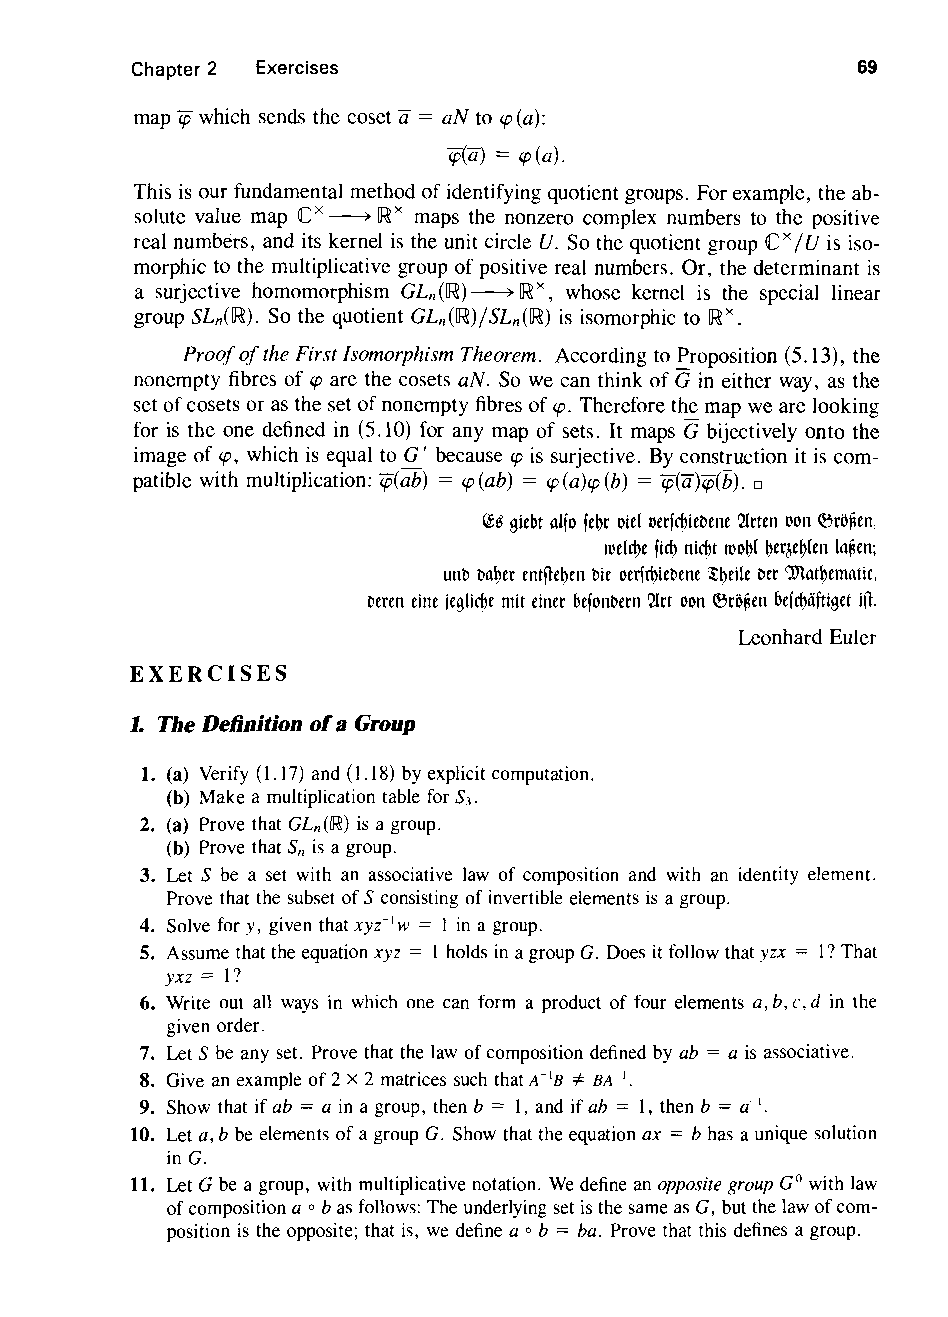
\includepdf[pages={1-},scale=0.85]{Exercises/C2_selection.pdf}
\section{The Definition of a Group}
%\documentclass[12pt]{article}
%\usepackage{amsmath, amssymb}
%\begin{document}
%\title{Chapter 2: Groups \\ Section 1: The Definition of a Group}
%\author{Alec Mouri}

%\maketitle
%\section*{Exercises}
\begin{itemize}
\item[(1)]
\begin{itemize}
\item[(a)]
$$1 = \begin{bmatrix}
1 & 0 & 0 \\
0 & 1 & 0 \\
0 & 0 & 1
\end{bmatrix}, x = \begin{bmatrix}
0 & 1 & 0 \\
0 & 0 & 1 \\
1 & 0 & 0
\end{bmatrix}, y = \begin{bmatrix}
0 & 1 & 0 \\
1 & 0 & 0 \\
0 & 0 & 1
\end{bmatrix}$$
$$x^2 = \begin{bmatrix}
0 & 0 & 1 \\
1 & 0 & 0 \\
0 & 1 & 0
\end{bmatrix}, xy = \begin{bmatrix}
1 & 0 & 0 \\
0 & 0 & 1 \\
0 & 1 & 0
\end{bmatrix}, x^2y = \begin{bmatrix}
0 & 0 & 1 \\
0 & 1 & 0 \\
1 & 0 & 0
\end{bmatrix}$$
$$x^3 = \begin{bmatrix}
1 & 0 & 0 \\
0 & 1 & 0 \\
0 & 0 & 1
\end{bmatrix}, y^2 = \begin{bmatrix}
1 & 0 & 0 \\
0 & 1 & 0 \\
0 & 0 & 1
\end{bmatrix}, yx = \begin{bmatrix}
0 & 0 & 1 \\
0 & 1 & 0 \\
1 & 0 & 0
\end{bmatrix} = x^2y$$
\item[(b)]
\begin{tabular}{| c || c | c | c | c | c | c |}
\hline
& 1 & $x$ & $x^2$ & $y$ & $xy$ & $x^2y$ \\
\hline \hline
1 & 1 & $x$ & $x^2$ & $y$ & $xy$ & $x^2y$ \\
\hline
$x$ & $x$ & $x^2$ & 1 & $xy$ & $x^2y$ & $y$ \\
\hline
$x^2$ & $x^2$ & 1 & $x$ & $x^2y$ & $y$ & $xy$ \\
\hline
$y$ & $y$ & $x^2y$ & $xy$ & 1 & $x^2$ & $x$ \\
\hline
$xy$ & $xy$ & $y$ & $x^2y$ & $x$ & 1 & $x^2$ \\
\hline
$x^2y$ & $x^2y$ & $xy$ & $y$ & $x^2$ & $x$ & $x^3$ \\
\hline
\end{tabular}
\end{itemize}
\item[(2)]
\begin{itemize}
\item[(a)]
Let $A, B, C \in GL(\mathbb{R})$. 

Note that $\det(AB) = \det(A)\det(B) \neq 0$, so $AB \in GL(\mathbb{R})$, so multiplication is a law of composition of $GL(\mathbb{R})$.

Further for $1 \leq i,j \leq n$,
$$((AB)C)_{ij} = \sum_{k=1}^n (AB)_{ik}c_{kj} = \sum_{k=1}^n\left(\sum_{m=1}^n a_{im}b_{mk}\right)c_{kj} $$
$$= \sum_{k=1}^n\sum_{m=1}^n a_{im}b_{mk}c_{kj} = \sum_{m=1}^na_{im}\left(\sum_{k=1}^n b_{mk}c_{kj}\right)$$
$$= \sum_{m=1}^na_{im}(BC)_{mj} = (A(BC))_{ij}$$
So multiplication is associative on $GL(\mathbb{R})$.

Note that $I \in GL(\mathbb{R})$, and $AI = IA = A$, so $GL(\mathbb{R})$ contains the identity matrix.

Since $\det A \neq 0$, then $A$ is invertible. Necessarily, $\det A^{-1} \neq 0$, and $AA^{-1} = A^{-1}A = I$, so $A$ has an inverse. 

Thus, $GL(\mathbb{R})$ is a group.
\item[(b)]
Let $X, Y, Z \in S_n$. Then for some $a, b, c \in 1...n$, $(XY)(a) = X(Y(a)) = X(b) = c$. So we have a law of composition of $S_n$.

Further,
$$((XY)Z)(a) = (XYZ)(a) = (X(YZ))(a)$$
So the law of composition is associative.

Note that $i \in S_n$, and $(Xi)(a) = X(i(a)) = X(a) = b$, and $(iX)(a) = i(X(a)) = i(b) = b$. so $S_n$ contains the identity permutation.

Suppose $X$ is a permutation such that $X(a) = b, X(b) = c$. Then there exists a permutation $Y$ such that $Y(b) = a, Y(c) = b$. So then $(XY)(b) = X(Y(b)) = X(a) = b$, and $(YX)(b) = Y(X(b)) = Y(c) = b$. Thus $X$ is invertible, and its inverse is $Y$.
\end{itemize}
\item[(3)]
Let $T = \left\lbrace s \in S | \text{\emph{s} is invertible} \right\rbrace$. Note that $I \in T$, since $II = I$. Let $t \in T$. $t$ is invertible, and has inverse $w$. Since $tw = I$, and $wt = I$, then $w$ is also invertible with inverse $t$. Thus, $w \in T$. Thus, since $T$ has an associative law of composition and the identity, then $T$ is a group.
\item[(4)]
$$xyz^{-1}w = 1 \rightarrow yz^{-1}w = x^{-1} \rightarrow yz^{-1} = x^{-1}w^{-1} \rightarrow y = x^{-1}w^{-1}z$$
\item[(5)]
$$xyz = 1 \rightarrow yz = x^{-1} \rightarrow yzx = 1$$
It does not follow that $yxz = 1$. Let $a = x, b = y, c = xy$. Then $abc = 1$. But $bac = yxxy = yx^2y = yyx = y^2x = x \neq 1$.
\item[(6)]
$$(abcd), a(bcd), (abc)d, (ab)(cd), (ab)cd, a(bc)d, ab(cd), abcd$$
\item[(7)]
Let $a, b, c \in S$. Then
$$(ab)c = ac = a = ab = a(bc)$$
Thus, the law of composition is associative.
\item[(8)]
Let $$A = \begin{bmatrix}
0 & 1 \\
1 & 0
\end{bmatrix}, B = \begin{bmatrix}
1 & 1 \\
0 & 0
\end{bmatrix}$$
Note that
$$A^{-1} = \begin{bmatrix}
0 & 1 \\
1 & 0
\end{bmatrix}$$
So
$$A^{-1}B = \begin{bmatrix}
0 & 0 \\
1 & 1
\end{bmatrix}$$
But
$$BA^{-1} = \begin{bmatrix}
1 & 1 \\
0 & 0
\end{bmatrix}$$
So $A^{-1}B \neq BA^{-1}$
\item[(9)]
$$ab = a \rightarrow a^{-1}ab = a^{-1}a \rightarrow b = 1$$
$$ab = 1 \rightarrow a^{-1}ab = a^{-1} \rightarrow b = a^{-1}$$
\item[(10)]
$$ax = b \rightarrow x = a^{-1}b$$
Since $a, b$ are distinct elements, then $x$ is unique.
\item[(11)]
Let $a, b, c \in G^\circ$. Since $a \circ b = ba \in G$, then $\circ$ is a law of composition in $G$. And,
$$(a \circ b) \circ c = (ba) \circ c = cba = (cb)a = a \circ (cb) = a \circ (b \circ c)$$
So $\circ$ is associative.

Since $I \in G$, then $a \circ I = Ia = a = aI = I \circ a$, so $I \in G^\circ$.

Let $a^{-1}$ be the inverse of $a$ in $G$. Then
$$a \circ a^{-1} = a^{-1}a = I = aa^{-1} = a^{-1} \circ a$$

So therefore $a$ has an inverse in $G^\circ$, namely $a^{-1}$. Thus $G^\circ$ is a group.
\end{itemize}
%\end{document}
\section{Subgroups}
%\documentclass[12pt]{article}
%\usepackage{amsmath, amssymb}
%\begin{document}
%\title{Chapter 2: Groups \\ Section 2: Subgroups}
%\author{Alec Mouri}
%
%\maketitle
%\section*{Exercises}
\begin{itemize}
\item[(1)]
$$x = \begin{bmatrix}
1 & 1 \\
-1 & 0
\end{bmatrix}, x^2 = \begin{bmatrix}
0 & 1 \\
-1 & -1
\end{bmatrix}, x^3 = \begin{bmatrix}
-1 & 0 \\
0 & -1
\end{bmatrix} $$
$$x^4 = \begin{bmatrix}
-1 & -1 \\
1 & 0
\end{bmatrix}, x^5 = \begin{bmatrix}
0 & -1 \\
1 & 1
\end{bmatrix}, x^6 = 1 = \begin{bmatrix}
1 & 0 \\
0 & 1
\end{bmatrix}$$
\item[(2)]
$$a^3b = ba^3 \rightarrow a^3a^3b = a^3ba^3 \rightarrow ab = a^5ab = a^3b^3$$
And
$$a^3b = ba^3 \rightarrow a^3ba^3 = ba^3a^3 \rightarrow a^3ba^3 = baa^5 = ba$$
Thus, $ab = ba$
\item[(3)]
\begin{itemize}
\item[(a)] Yes. $GL_N(\mathbb{R})$ is a group, so it is a subgroup of $GL_N(\mathbb{C})$.
\item[(b)] Yes. Let $A, B \in \left\lbrace 1, -1 \right\rbrace$. Clearly, $AB \in \left\lbrace 1, -1 \right\rbrace$. And, $1 \in \left\lbrace 1, -1 \right\rbrace$, $1^{-1} = 1$, and $(-1)^{-1} = -1$. So, $\left\lbrace 1, -1 \right\rbrace$ is a subgroup of $\mathbb{R}^\times$.
\item[(c)] No. Let $\mathcal{A}$ be the set of positive integers in $\mathbb{Z}^+$. For $a \in \mathcal{A}$ where $a \neq 0$, $-a \not \in \mathcal{A}$. So $\mathcal{A}$ is not a subgroup.
\item[(d)]Yes. Let $\mathcal{A}$ be the set of positive reals in $\mathbb{R}^\times$. For $a, b \in \mathcal{A}$, clearly $ab \in \mathcal{A}$. And, $1 \in \mathcal{A}$. For $a \in \mathcal{A}$, since $a^{-1} > 0$, then $a^{-1} \in \mathcal{A}$. so $\mathcal{A}$ is a subgroup of $\mathbb{R}^\times$.
\item[(e)] No. Let $a = 1$. Then
$$\begin{bmatrix}
1 & 0 \\
0 & 0
\end{bmatrix} \not \in GL_2(\mathbb{R})$$
Since
$$\det\begin{bmatrix}
1 & 0 \\
0 & 0
\end{bmatrix} = 0$$
\end{itemize}
\item[(4)]
Let $x \in H$. Since $1 = xx^{-1} \in H$, then $H$ contains the identity. And, since $x^{-1} = 1x^{-1} \in H$, then $H$ is closed under inverses. Let $x, y \in H$. Then $y^{-1} \in H$. Then $xy = x(y^{-1})^{-1} \in H$. Thus, $H$ is a subgroup of $G$.
\item[(5)]
Let $\mathcal{A}$ be the $n$th roots of unity. Let $a, b \in \mathcal{A}$. Since $(ab)^n = a^nb^n = 1$, then $ab \in \mathcal{A}$. And, since $1^n = 1$, then $1 \in \mathcal{A}$. And, $(a^{-1})^n = (a^n)^{-1} = 1^{-1} = 1$. Thus $\mathcal{A} \subseteq \mathbb{C}^\times$. There are $n$ such roots: $z = e^{\frac{2\pi k}{n}}$ for $k = 0, ..., n - 1$. $\mathcal{A}$ is generated by $z = e^{\frac{2\pi}{n}}$, so $\mathcal{A}$ is a cyclic subgroup of order $n$.
\item[(6)]
\begin{itemize}
\item[(a)]
Let
$$a = \begin{bmatrix}
-1 & \\
& 1
\end{bmatrix}, b = \begin{bmatrix}
1 & \\
& -1
\end{bmatrix}$$
$a^2 = b^2 = I$, and $ab = ba$.
\item[(b)]
For each of the following sets the identity matrix is contained, they are closed under multiplication, and they are closed under inverses (in particular, the inverse of any matrix in the Klein four group is itself). Thus, the subgroups of the Klein four group are:
$$\left\lbrace \begin{bmatrix}
1 & \\
& 1
\end{bmatrix} \right\rbrace, \left\lbrace \begin{bmatrix}
\pm 1 & \\
& \pm 1
\end{bmatrix} \right\rbrace, \left\lbrace \begin{bmatrix}
1 & \\
& 1
\end{bmatrix}, \begin{bmatrix}
-1 & \\
& -1
\end{bmatrix} \right\rbrace$$
$$\left\lbrace \begin{bmatrix}
\pm 1 & \\
& 1
\end{bmatrix} \right\rbrace, \left\lbrace \begin{bmatrix}
1 & \\
& \pm 1
\end{bmatrix} \right\rbrace$$
\end{itemize}
\item[(7)]
\begin{itemize}
\item[(a)]
Let $ar + bs, ax + by \in a\mathbb{Z} + b\mathbb{Z}$. Then $ar + bs + ax + by = a(r + x) + b(s + y) \in a\mathbb{Z} + b\mathbb{Z}$.

Further, $0 = 0r + bs \in a\mathbb{Z} + b\mathbb{Z}$, and $ar + bs + a(-r) + b(-s) = 0$, so $a\mathbb{Z} + b\mathbb{Z}$ is closed under inverses. Thus, $a\mathbb{Z} + b\mathbb{Z}$ is a subgroup of $\mathbb{Z}^+$.
\item[(b)]
Let $c = ar + bs \in a\mathbb{Z} + b\mathbb{Z}$. Then 
$$c = ar + bs = s(b + 7a) + ar - 7as = s(b + 7a) + (r - 7s)a$$
Thus, $a\mathbb{Z} = b\mathbb{Z}$ is generated by $a$ and $b + 7a$.
\end{itemize}
\item[(8)]
\begin{tabular}{|c||c|c|c|c|}
\hline
& $1$ & $i$ & $j$ & $k$ \\
\hline
\hline
$1$ & $1$ & $i$ & $j$ & $k$ \\
\hline
$i$ & $i$ & $-1$ & $k$ & $-j$ \\
\hline
$j$ & $j$ & $-k$ & $-1$ & $i$ \\
\hline
$k$ & $k$ & $j$ & $-i$ & $-1$ \\
\hline
\end{tabular}
\item[(9)]
Let $x \in H$. Then we can write $x$ has a string of products of $a$ and $b$ and their inverses. Ie. $x = a^{a_1}b^{b_1}...a^{a_n}b^{b_n}$, where $a_n, b_n$ are integers. Since $ab = ba$ and hence $a^{-1}b^{-1} = b^{-1}a^{-1}$, $ab^{-1} = b^{-1}a$, and $a^{-1}b = ba^{-1}$, then we can also write $x = a^{a_1+...+a_n}b^{b_1+...+b_n} = a^{b_1 + ... + b-n}a^{a_1+...+a_n}$, or equivalently for some integers $c, d$, $x = a^cb^d = b^da^c$. 

So, let $x = a^{x_a}b^{x_b}, y = a^{y_a}b^{y_b} \in H$, where $x_a, x_b, y_a, y_b$ are integers. Then
$$xy = a^{x_a}b^{x_b}a^{y_a}b^{y_b} = a^{y_a}b^{y_b}a^{x_a}b^{x_b} = yx$$
Thus, $H$ is abelian.
\item[(10)]
\begin{itemize}
\item[(a)]
If $x$ has order $rs$, then $(x^r)^s = x^{rs} = 1$. Suppose for some $k < s$, $(x^r)^k = 1$. Then this implies $x^{rk} = 1$. But $rk < rs$, so $rs$ is not the order of $x$. Contradiction. Thus $s$ is the order of $x^r$.
\item[(b)]
If $x$ has order $n$, then for some $s$ and $k$ such that $rs = kn$, then $(x^r)^s = x^{rs} = x^{kn} = (x^n)^k = 1$. Choose $k$ such that $k = r/\text{gcd}(n, r)$. Then $r$ divides $kn$, so $s$ is an integer, namely $s = n/\text{gcd}(n,r)$. We now claim that $s$ is the order of $x^r$. Let $a$ be the order of $x^r$. Then $a$ divides $s$. Since $(x^r)^a = x^{ra} = 1$, then $n$ divides $ra$. Since $n/\text{gcd}(n,r)$ does not divide $r$ unless $\text{gcd}(n,r) = n$ or $r = 1$, then $s = n/\text{gcd}(n,r)$ divides $a$. Thus, $s = a$.
\end{itemize}
\item[(11)]
Let $|ab| = n$. Then $1 = (ab)^n = a(ba)^{n-1}b \rightarrow a^{-1}b^{-1} = (ba)^{n-1} \rightarrow (ba)^{-1} = (ba)^{n-1} \rightarrow 1 = (ba)^n$. Suppose now that $|ba| = m$, so that $n \geq m$. We can similarly show that $(ab)^m = 1$, so then $n \leq m$. Thus, $n = m$.
\item[(12)]
Clearly, the trivial group has no proper subgroup.

Suppose we have a nontrivial group $G$ with no proper subgroup. So for all $g \in G$ where $g \neq e$, where $e$ is the identity, $g$ generates $G$. Suppose $|G| = \infty$. Then $g^2$ generates a nontrivial subgroup, since it does not contain $g$. Thus, for $|G| < \infty$, $G = \left\lbrace e, g, g^2, ..., g^{|G| - 1} \right\rbrace$. Furthermore, for all $1 \leq k \leq |G| - 1$, $G = \left\lbrace e, g^k, (g^k)^2, ..., (g^k)^{|G|-1} \right\rbrace$, where for each $i$, $g^{ik} \neq 1$. Suppose $|G|$ is composite. Then for some $k$ and $a$, $|G| = ka$. Thus, $(g^k)^a = 1$. Thus, $|G|$ must be prime.

So, a nontrivial group $G$ with no proper subgroup is a cyclic subgroup with prime order.
\item[(13)]
Let $G$ be a cyclic group with generator $g$, and let $A$ be a subgroup of $G$. Then for some $a \in A, a = g^k$ for some $k$, and $a$ has order $n$. Suppose for some $b \in A$, $b$ is not generated by $a$, and $a$ is not generated by $b$. Then for some $\ell$, $b = g^\ell$, where $\text{gcd}(k, \ell) = 1$, and $b$ has order $m$. But since for some $c, d$, $g^{ck + d\ell} = g$, then $A = G$, so $A$ is cyclic. Thus, $b$ is generated by $a$, or $a$ is generated by $b$. Thus, $A$ is a cyclic group.
\item[(14)]
Suppose $G$ is generated by $g$, and $n = pr$ for some $p$. Note that $\mathcal{A} = \left\lbrace e, g^p, ..., g^{p(r-1)} \right\rbrace$ is a cyclic subgroup of $G$ of order $r$ generated by $g^p$. I claim that $\mathcal{A}$ is the only cyclic subgroup of $G$ of order $r$. Suppose there exists some other subgroup of $G$, $\mathcal{B}$, where the order of $\mathcal{B}$ is $r$, and $\mathcal{B}$ is generated by $g^q$ for some $q$. Then $(g^q)^r = g^{qr} = 1$. So $n$ divides $qr$, and so $p$ divides $q$. But then $g^p$ generates $g^q$. So, $\mathcal{B}$ is generated by $g^p$. Thus, $\mathcal{A} = \mathcal{B}$.
\item[(15)]
\begin{itemize}
\item[(a)]
Let $e$ be the identity of $H$ and $f$ be the identity of $G$. Then $e^2 = e = ef \rightarrow e = f$.
\item[(b)]
Let $a, b \in H, c \in G$, where $b$ is the inverse of $a$ in $H$, and $c$ is the inverse of $a$ in $G$. Then $e = ab = ac \rightarrow bab = bac \rightarrow b = c$.
\end{itemize}
\item[(16)]
\begin{itemize}
\item[(a)]
Let $G = \left\lbrace 1, g, g^2, g^3, g^4, g^5 \right\rbrace$. Since $1^1 = 1, g^6 = 1, (g^2)^3 = 1, (g^3)^2 = 1, (g^4)^3 = 1, (g^5)^6 = 1$, then $g$ and $g^5$ generate $G$
\item[(b)]
Let $A = \left\lbrace 1, a, a^2, a^3, a^4 \right\rbrace$. Since $1^1 = 1, a^5 = 1, (a^2)^5 = 1, (a^3)^5 = 1, (a^4)^5 = 1$, then $a, a^2, a^3, a^4$ generate $A$.

Let $B = \left\lbrace 1, b, b^2, b^3, b^4, b^5, b^6, b^7 \right\rbrace$. Since $1^1 = 1, b^8 = 1, (b^2)^4 = 1, (b^3)^8 = 1, (b^4)^2 = 1, (b^5)^8 = 1, (b^6)^4 = 1, (b^7)^8 = 1$, then $b, b^3, b^5, b^7$ generate $B$.

Let $C = \left\lbrace 1, c, c^2, c^3, c^4, c^5, c^6, c^7, c^8, c^9 \right\rbrace$. Since $1^1 = 1, c^{10} = 1, (c^2)^5 = 1, (c^3)^{10} = 1, (c^4)^5 = 1, (c^5)^2 = 1, (c^6)^5 = 1, (c^7)^{10} = 1, (c^8)^5 = 1, (c^9)^{10} = 1$, then $c, c^3, c^7, c^9$ generate $C$.
\item[(c)] If $g$ generates $G$ and has order $n$, then $g^k$ generates $G$ if $\text{gcd}(k, n) = 1$.
\end{itemize}
\item[(17)]
Let $a, b \in G$. Then $a^2 = b^2 = 1 \rightarrow a = a^{-1}, b = b^{-1}$. Furthermore, $(ab)^2 = 1 \rightarrow ab = (ab)^{-1}$. Then
$$a = a^{-1}, b = b^{-1} \rightarrow ab = a^{-1}b^{-1} = (ba)^{-1} = ba$$
\item[(18)]
\begin{itemize}
\item[(a)]
Let $A$ be an elementary matrix of the second kind whose operation is interchanging rows $i$ and $j$. Ie.
$$A = \begin{bmatrix}
1 \\
& \ddots \\
& & 0 & & 1 \\
& & & \ddots \\
& & 1 & & 0 \\
& & & & & \ddots \\
& & & & & & 1
\end{bmatrix}$$
Let
$$E_1 = \begin{bmatrix}
1 \\
& \ddots \\
& & 1 \\
& & & \ddots \\
& & & & -1 \\
& & & & & \ddots \\
& & & & & & 1
\end{bmatrix}$$
$$E_2 = \begin{bmatrix}
1 \\
& \ddots \\
& & 1 \\
& & & \ddots \\
& & -1 & & 1 \\
& & & & & \ddots \\
& & & & & & 1
\end{bmatrix}$$
$$E_3 = \begin{bmatrix}
1 \\
& \ddots \\
& & 1 & & 1 \\
& & & \ddots \\
& & & & 1 \\
& & & & & \ddots \\
& & & & & & 1
\end{bmatrix}$$
Ie. $E_1$ scales row $j$ by -1, $E_2$ sets row $j$ equal to row $j$ minus row $i$, and $E_3$ sets row $i$ equal to row $i$ plus row $j$. Then $A = E_1E_2E_3E_2$. So, we can write an elementary matrix of the second kind as a product of elementary matrices of the first and third kinds. So then we can generate any invertible matrix with elementary matrices of the first and third kinds.
\item[(b)]
Clearly, $SL_n(\mathbb{R}) \subseteq GL_n(\mathbb{R})$. Let $A, B \in SL_n(\mathbb{R})$. Since $\det(AB) = \det(A)\det(B) = 1$, then $AB \in SL_n(\mathbb{R})$. Since $I_n \in SL_n(\mathbb{R})$, and $\det(A^{-1}) = \det(A)^{-1} = 1$, then $A^{-1} \in SL_n(\mathbb{R})$. Thus, $SL_n(\mathbb{R})$ is a subgroup of $GL_n(\mathbb{R})$. 
\item[(c)]
Consider the $2 \times 2$ matrix
$$A = \begin{bmatrix}
a & b \\
c & d
\end{bmatrix}$$
Since $\det A = 1$, then $ad - bc = 1$.

If $c \neq 0$, then reducing $A$:
$$\begin{bmatrix}
a & b \\
c & d
\end{bmatrix} \rightarrow \begin{bmatrix}
1 & b + d(1-a)/c \\
c & d
\end{bmatrix} \rightarrow \begin{bmatrix}
1 & b + d(1-a)/c \\
& ad - bc
\end{bmatrix} \rightarrow \begin{bmatrix}
1 & \\
& 1
\end{bmatrix} $$

If $c = 0$, then $a \neq 0$ (otherwise $\det A = 0$). Then:
$$\begin{bmatrix}
a & b \\
& d
\end{bmatrix} \rightarrow \begin{bmatrix}
a & b \\
1 - a & d + b(1 - a)/a
\end{bmatrix} \rightarrow \begin{bmatrix}
1 & d + b/a \\
1 - a & d + b(1 - a)/a
\end{bmatrix}$$
$$\rightarrow \begin{bmatrix}
1 & d + b/a \\
& ad
\end{bmatrix} \rightarrow \begin{bmatrix}
1 & \\
& 1
\end{bmatrix}$$
$A$ was reduced only with type 1 operations, so we can write $A$ as a product of elementary matrices of the first kind. 

Suppose for all $X \in SL_{n-1}(\mathbb{R})$ we can write $X$ as a product of elementary matrices of the first kind. Now consider an $n \times n$ matrix $B$. Suppose $b_{21} = ... = b_{n1} = 0$. Then $b_{11} \neq 0$ (otherwise $\det B = 0$). The following operations set $b_{11} = 1$ while keeping $b_{21} = ... = b_{n1} = 0$:
$$ \begin{bmatrix}
1 & 1 \\
& 1 \\
& & \ddots \\
& & & 1
\end{bmatrix}\begin{bmatrix}
1 \\
(1-b_1)/b_1 & 1 \\
& & \ddots \\
& & & 1
\end{bmatrix}$$
Suppose now that $b_{11} = 0$. Then for some $b_{i1}$, $b_{i1} \neq 0$. Then the following operation sets $b_{11} = 1$:
$$\begin{bmatrix}
1 & & 1/b_{i1} \\
& \ddots \\
& & 1 \\
& & & \ddots \\
& & & & 1
\end{bmatrix}$$
If $b_{11} = 1$, then we can perform type 1 operations to set $b_{21} = ... = b_{n1} = 0$: namely if $b_{i1} \neq 0$, then we can perform the following operation:
$$\begin{bmatrix}
1 \\
& \ddots \\
-b_{i1} & & 1 \\
& & & \ddots \\
& & & & 1
\end{bmatrix}$$
After applying the above operations, now $b_{11} = 1$ and $b_{21} = ... = b_{n1} = 0$. Consider the submatrix $B_{11}$. Since $1 = \det B = b_{11}\det B_{11}$, then $\det B_{11} = 1$, since $B_{11} \in SL_{n-1}(\mathbb{R})$. By the inductive hypothesis, there exists a series of type 1 matrices such that $B_{11}$ can be reduced to the identity. So, $B$ can be reduced to an upper triangular matrix $B'$ with 1s as its diagonal entries. Now we can apply type one operations to clear the entries above the diagonal, so that $B'$ is row reduced to the identity. Since for elementary matrices of the first kind $E_1, ..., E_p$ exist such that $E_1...E_pB = I$, then $B = E_p^{-1}...E_1^{-1}$ is a product of elementary matrices of the first kind. Thus elementary matrices of the first kind generate $SL_n(\mathbb{R})$.
\end{itemize}
\item[(19)]
$$\begin{bmatrix}
& 1 \\
1 & \\
& & 1 \\
& & & 1
\end{bmatrix}, \begin{bmatrix}
& & 1 \\
& 1 \\
1 \\
& & & 1
\end{bmatrix}, \begin{bmatrix}
& & & 1 \\
& 1 \\
& & 1 \\
1
\end{bmatrix}$$
$$\begin{bmatrix}
1 \\
& & 1 \\
& 1 \\
& & & 1
\end{bmatrix}, \begin{bmatrix}
1 \\
& & & 1 \\
& & 1 \\
& 1
\end{bmatrix}, \begin{bmatrix}
1 \\
& 1 \\
& & & 1 \\
& & 1
\end{bmatrix}$$
$$\begin{bmatrix}
& 1 \\
1 \\
& & & 1 \\
& & 1
\end{bmatrix}, \begin{bmatrix}
& & 1 \\
& & & 1 \\
1 \\
& 1
\end{bmatrix}, \begin{bmatrix}
& & & 1 \\
& & 1 \\
& 1 \\
1
\end{bmatrix}$$
There are 9 elements with order 2 in $S_4$.
\item[(20)]
\begin{itemize}
\item[(a)]
Note that 
$$(ab)^{nm/\text{gcd}(n,m)} = a^{nm/\text{gcd}(n,m)}b^{nm/\text{gcd}(n,m)}$$
$$= (a^m)^{n/\text{gcd}(n,m)}(b^n)^{m/\text{gcd}(n,m)} = 1$$ So $ab$ has finite order as most $\frac{nm}{\text{gcd}(n,m)}$. 
\item[(b)]
Consider
$$A = \begin{bmatrix}
0 & 1 \\
-1 & 0
\end{bmatrix}, B = \begin{bmatrix}
0 & -1 \\
1 & 1
\end{bmatrix}$$
Note that $A^4 = I, B^6 = I$. But
$$AB = \begin{bmatrix}
1 & 1 \\
& 1
\end{bmatrix}, (AB)^n = \begin{bmatrix}
1 & n \\
& 1
\end{bmatrix}$$
So, $AB$ does not have finite order.
\end{itemize}
\item[(21)]
From the previous exercise, then if $a, b \in G$, where $G$ is an abelian group and $a, b$ have finite order, then $ab$ also has finite order. Let $H$ be the subset of $G$ whose elements have finite order. Clearly, $e \in H$, where $e$ is the identity. And, for $a \in H$, where $|a| = n$, then $a^{-1} = a^{n-1}$. So, $H$ is a subgroup of $G$.
\item[(22)]
Let $a = p_1^{a_1}...p_n^{a_n}, b = p_1^{b_1}...p_n^{b_n}$, where $p_1...p_n$ are primes and $a_1, ..., a_n, b_1, ..., b_n \geq 0$. Such product of primes is unique by the Fundamental Theorem of Arithmetic. Let $g$ be the greatest common divisor of $a$ and $b$. Since $g$ divides $a$ and $g$ divides $b$, then $g = p_1^{c_1}...p_n^{c_n}$, where for all $i$, $c_i \geq 0, c_i \leq a_i, c_i \leq b_i$. Suppose some integer $h$ also divides $a$ and $b$. Then $h = p_1^{d_1}...p_n^{d_n}$. Then $g$ also divides $h$. So for all $i$, $c_i \geq d_i$, ie. $c_i$ is the largest integer such that $c_i \leq a_i$ and $c_i \leq b_i$. Thus, $g = p_1^{\min(a_1,b_1)}...p_n^{\min(a_n,b_n)}$.
\end{itemize}
%\end{document}
\section{Isomorphisms}
%\documentclass[12pt]{article}
%\usepackage{amsmath, amssymb}
%\begin{document}
%\title{Chapter 2: Groups \\ Section 3: Isomorphisms}
%\author{Alec Mouri}
%
%\maketitle
%\section*{Exercises}
\begin{itemize}
\item[(1)]
Let $\varphi(x) = 2^x$. Then for $a, b \in \mathbb{R}^+$, $\varphi(a + b) = 2^{a + b} = 2^a2^b = \varphi(a)\varphi(b)$. Since $2^x > 0$ for all $x$, then $\varphi$ is injective. And, $\log_2(2^x) = x$, so $\varphi$ is surjective, and is therefore bijective. So, $\varphi$ is an isomorphism from $\mathbb{R}^+$ to $P$. Thus, $\mathbb{R}^+$ and $P$ are isomorphic.
\item[(2)]
$a(ba)a^{-1} = ab$, so $ab$ and $ba$ are conjugate elements.
\item[(3)]
Suppose $a = a'$. Then
$$a = bab^{-1} \rightarrow ab = ba$$
Now suppose $ab = ba$. Then
$$ab = ba \rightarrow b^{-1}ab = a \rightarrow a = a'$$
\item[(4)]
\begin{itemize}
\item[(a)]
Suppose for $n - 1 \geq 1$, $b'^{n-1} = ab^{n-1}a^{-1}$. Then 
$$b'^n = (aba^{-1})^n = aba^{-1}(aba^{-1})^{n-1} = aba^{-1}ab^{n-1}a^{-1} = ab^na^{-1}$$
If $n = 0$, Then $ab^0a^{-1} = 1 = b'^0$.

If $n \leq -1$, then
$$b'^n = (b^{-n})^{-1} = (ab^{-n}a^{-1})^{-1} = ab^{n}a^{-1}$$
\item[(b)]
Note that $ab = b^2a$. Then
$$a^3ba^{-3} = a^2b^2a^{-2} = ab^2aba^{-2} = ab^4a^{-1} = b^8$$
\end{itemize}
\item[(5)]
Since $\varphi$ is a bijection, then $\varphi^{-1}$ is also a bijection. And, for $c, d \in G'$, then for some $a, b \in G$, $\varphi(a) = c$ and $\varphi(b) = d$. Then 
$$\varphi^{-1}(cd) = \varphi^{-1}(\varphi(a)\varphi(b)) = \varphi^{-1}(\varphi(ab)) = ab = \varphi^{-1}(c)\varphi^{-1}(d)$$
Thus, $\varphi^{-1}$ is an isomorphism.
\item[(6)]
\begin{itemize}
\item[(a)]
Let $n, m$ be the orders of $x$ and $x'$ respectively. Then
$$1 = \varphi(1) = \varphi(x^n) = \varphi(x)^n = x'^n$$
So $m \leq n$. But
$$1 = x'^m = \varphi(x)^m = \varphi(x^m) \rightarrow x^m = 1$$
So, $n \leq m$. Therefore, $n = m$.
\item[(b)]
$$x'y'x' = \varphi(x)\varphi(y)\varphi(x) = \varphi(xyx) = \varphi(yxy)$$
$$= \varphi(y)\varphi(x)\varphi(y) = y'x'y'$$
\item[(c)]
Since
$$1 = \varphi(1) = \varphi(xx^{-1}) = \varphi(x)\varphi(x^{-1})$$
Then
$$\varphi(x^{-1}) = \varphi(x)^{-1} = x'^{-1}$$
\end{itemize}
\item[(7)]
Note that
$$\begin{bmatrix}
& 1 \\
1 &
\end{bmatrix}\begin{bmatrix}
1 & 1 \\
& 1
\end{bmatrix}\begin{bmatrix}
& 1 \\
1 &
\end{bmatrix} = \begin{bmatrix}
& 1 \\
1
\end{bmatrix}\begin{bmatrix}
1 & 1 \\
1
\end{bmatrix} = \begin{bmatrix}
1 \\
1 & 1
\end{bmatrix}$$
Thus,
$$\begin{bmatrix}
1 & 1 \\
& 1
\end{bmatrix}\begin{bmatrix}
1 \\
1 & 1
\end{bmatrix}$$
are conjugate elements in $GL_2(\mathbb{R})$.
Now, let
$$A = \begin{bmatrix}
a & b \\
c & d
\end{bmatrix} \in SL_2(\mathbb{R})$$
Then
$$A^{-1} = \begin{bmatrix}
d & -b \\
-c & a
\end{bmatrix}$$
So if the two matrices are conjugate, then now we have
$$\begin{bmatrix}
1 & \\
1 & 1
\end{bmatrix} = \begin{bmatrix}
a & b \\
c & d
\end{bmatrix}\begin{bmatrix}
1 & 1 \\
& 1
\end{bmatrix}\begin{bmatrix}
d & -b \\
-c & a
\end{bmatrix}$$ 
$$= \begin{bmatrix}
a & b \\
c & d
\end{bmatrix}\begin{bmatrix}
d - c & a - b \\
-c & a
\end{bmatrix} = \begin{bmatrix}
ad - ac - bc & a^2 \\
-c^2 & ac + ad - bc
\end{bmatrix} $$
$$= \begin{bmatrix}
-ac & a^2 \\
-c^2 & ac
\end{bmatrix}$$
So, we have $1 = ac$ and $a^2 = 0$. So $a = 0$. But then we have $1 = 0$, a contradiction. Thus, they are not conjugate in the group $SL_n(\mathbb{R})$.
\item[(8)]
Let
$$A = \begin{bmatrix}
1 & 3 \\
& 1
\end{bmatrix}, A^{-1} = \begin{bmatrix}
1 & -3 \\
& 1
\end{bmatrix}$$
Then
$$\begin{bmatrix}
1 & 3 \\
& 1
\end{bmatrix}\begin{bmatrix}
1 \\
& 2
\end{bmatrix}\begin{bmatrix}
1 & -3 \\
& 1
\end{bmatrix} = \begin{bmatrix}
1 & 3 \\
& 1
\end{bmatrix}\begin{bmatrix}
1 & -3 \\
& 2
\end{bmatrix} = \begin{bmatrix}
1 & 3 \\
& 2
\end{bmatrix}$$
So,
$$\begin{bmatrix}
1 \\
& 2
\end{bmatrix}, \begin{bmatrix}
1 & 3 \\
& 2
\end{bmatrix}$$
are conjugate elements in $GL_2(\mathbb{R})$.
\item[(9)]
Denote $\cdot$ to be the group operation of $G^0$. Consider $\varphi(x) = x^{-1}$. Since $x = \varphi(x)^{-1}$, then $\varphi$ is a bijection. Then for $a, b \in G$,
$$\varphi(ab) = (ab^{-1}) = b^{-1}a^{-1} = a^{-1} \cdot b^{-1} = \varphi(a) \cdot \varphi(b)$$
Thus, $\varphi$ is an isomorphism between $G$ and $G^0$.
\item[(10)]
Denote $\varphi(A) = (A^\top)^{-1}$. Since 
$$\varphi(A^\top)^{-1}) = (((A^\top)^{-1})^\top)^{-1} = (((A^\top)^{-1})^{-1})^\top = A$$
Then $\varphi$ is a bijection. Then for $A, B \in GL_n(\mathbb{R})$,
$$\varphi(AB) = ((AB)^\top)^{-1} = (B^\top A^\top)^{-1} = (A^\top)^{-1}(B^\top)^{-1} = \varphi(A)\varphi(B)$$
Thus, $\varphi$ is an automorphism of $GL_n(\mathbb{R})$.
\item[(11)]
Consider $\varphi, \tau \in \text{Aut }G$. Let $a, b \in G$. Then
$$(\varphi \circ \tau)(ab) \varphi(\tau(a)\tau(b)) = \varphi(\tau(a))\varphi(\tau(b)) = (\varphi \circ \tau)(a)(\varphi \circ \tau)(b)$$
Furthermore, $\varphi^{-1}$ and $\tau^{-1}$ exist since $\varphi$ and $\tau$ are bijections. Then $((\tau^{-1} \circ \varphi^{-1}) \circ (\varphi \circ \tau))(a) = a$, so $\varphi \circ \tau$ is a bijection. Therefore, function composition is a law of composition of $\text{Aut }G$. Further, function composition is associative. 

Let $e$ be the trivial automorphism, ie. $e(a) = a$. Note that $\varphi \circ e = e \circ \varphi$. So, $e$ is the identity automorphism.

Further, $\varphi \circ \varphi^{-1} = \varphi^{-1} \circ \varphi = e$. so $\text{Aut }G$ is closed under inverses, and is therefore a group.
\item[(12)]
\begin{itemize}
\item[(a)]
$\varphi(x^{-1} = x$, so $\varphi$ is bijective.
\item[(b)]
Suppose $\varphi$ is an automorphism. Then for $x, y \in G$, then
$$y^{-1}x^{-1} = \varphi(xy) = \varphi(x)\varphi(y) = x^{-1}y^{-1} \rightarrow xy = yx$$
So, $G$ is abelian.

Now suppose $G$ is abelian. Then
$$\varphi(xy) = (xy)^{-1} = (yx)^{-1} = x^{-1}y^{-1} = \varphi(x)\varphi(y)$$
So, $\varphi$ is an automorphism.
\end{itemize}
\item[(13)]
\begin{itemize}
\item[(a)]
Suppose for some $a \in G$, that $a^n = 1$, where $n > 4$. Then $1, a, a^2, a^3, a^4$ are all distinct (if $a^i = a^j$ for some $i, j$, $n > j > i$, then $a^{j - i} = 1$, so $|a| < n$). So, $|G| \geq 5$, a contradiction. Thus, $n \leq 4$. Suppose $n = 3$. Then for some $b \in G$, $1 \neq a \neq a^2 \neq b$. Consider the product $ab$. If $ab = b$, then $a = 1$, a contradiction. For $i = 1,2$, if $ab = a^i$, then $b = a^{i - 1}$, a contradiction. And, if $ab = 1$, then $b = a^{-1} = a^2$, a contradiction. Therefore, $ab \not \in G$, so therefore if $G$ has order 4, then no element can have order 3.
\item[(b)]
\begin{itemize}
\item[(i)]
Consider $a \in G$, where $|a| = 4$. Then $1, a, a^2, a^3$ are distinct. Since $|G| = 4$, then $a$ generates $G$, so $G$ is a cyclic group of order 4.
\item[(ii)]
Consider $a \in G$. If $a^1 = 1$, then $a = 1$. If $a^2 = 1$, then $a = a^{-1}$. So, the elements of $G$ are their own inverses.
\end{itemize}
\end{itemize}
\item[(14)]
\begin{itemize}
\item[(a)]
Let $\varphi$ be an automorphism of $\mathbb{Z}^+$. Note that for $n \in \mathbb{Z}^+$,
$$\varphi(n) = \varphi(n1) = n\varphi(1)$$
So, if $\varphi(1) = a$, then $an = \varphi(n)$, ie. $\varphi$ is determined by the mapping $1 \mapsto a$. Furthermore, since $\varphi^{-1}(n) = \frac{n}{a}$, then $\frac{1}{a}$, then for all $n$, $a$ divides $n$. Thus, $a = 1, -1$. So, $\varphi$ is the mapping determined by $1 \mapsto \left\lbrace -1, 1 \right\rbrace$.
\item[(b)]
Let $G$ be a cyclic group of order 10 generated by $g$. For an automorphism $\varphi$ of $G$ and $x \in G$, then $|x| = |\varphi(x)|$. So, $g$ maps to one of $g, g^3, g^7, g^9$. Then for all $i$, $\varphi(g^i) = \varphi(g)^i = g^{ik}$, where $k = 1, 3, 7, 9$. For $i, j$, if $g^{ik} = g^{jk}$, then $g^{k(j - i)} = 1$. Then $j = i$, so therefore each $g^{ik}$ is distinct. Thus, $\varphi$ is the mapping determined by $g \mapsto \left\lbrace g, g^3, g^7, g^9 \right\rbrace$.
\item[(c)]
Let
$$x = \begin{bmatrix}
& 1 \\
& & 1 \\
1
\end{bmatrix}, y = \begin{bmatrix}
& 1 \\
1 \\
& & 1
\end{bmatrix}$$
Let $\varphi$ be an automorphism of $S_3$. Then for $0 \leq i \leq 2,  0\leq j \leq 1$, 
$$\varphi(x^iy^j) = \varphi(x)^i\varphi(y)^j$$
Ie. $\varphi$ is determined by $\varphi(x)$ and $\varphi(y)$. Since $|x| = |x^2|$ and $|y| = |xy| = |x^2y|$, then $x$ maps to one of $x, x^2$, and $y$ maps to one of $y, xy, x^2y$. Thus, $\varphi$ is the mapping determined by $x \mapsto \left\lbrace x, x^2 \right\rbrace$ and $y \mapsto \left\lbrace y, xy, x^2y \right\rbrace$.
\end{itemize}
\item[(15)]
First, denote $e(x) = x$. Note that for some function $f$, $e(f(x)) = f(x) = f(e(x))$, so $e(x)$ is an identity function. Further,
$$f^2(x) = \frac{1}{\frac{1}{x}} = x = e(x)$$
$$g^2(x) = \frac{\frac{x-1}{x} - 1}{\frac{x-1}{x}} = \frac{x- 1 - x}{x - 1} = \frac{-1}{x-1}$$
$$g^3(x) = \frac{\frac{-1}{x-1}-1}{\frac{-1}{x-1}} = \frac{-1 - (x-1)}{-1} = x = e(x)$$
$$(g \circ f)(x) = \frac{\frac{1}{x} - 1}{\frac{1}{x}} = \frac{1 - x}{x}$$
$$(g^2 \circ f)(x) = \frac{-1}{\frac{1}{x} - 1} = \frac{-x}{1 - x}$$
$$(f \circ g)(x) = \frac{1}{\frac{x-1}{x}} = \frac{x}{x-1} = (g^2 \circ f)(x)$$
So, $f$ has order 2 and $g$ has order 3. So, we can write any composition of functions as $g^if^j$, where $0 \leq i \leq 2, 0 \leq j \leq 1$. Define $\varphi$ such that $\varphi(f) = y$ and $\varphi(g) = x$ and $\varphi(g^if^j) = x^iy^j$. Since $\varphi^{-1}(x^iy^j) = g^if^j$, then $\varphi$ is a bijection. Then let $(g^af^b)(g^cf^d) = g^mf^n$, so then $(x^ay^b)(x^ay^b) = x^my^n$. Then $$\varphi((g^af^b)(g^cf^d)) = \varphi(g^mf^n) = x^my^n = (x^ay^b)(x^cy^d) = \varphi(g^af^b)\varphi(g^cf^d)$$
So $f$ and $g$ generates a group $G$ where $G$ is isomorphic to $S_3$.
\item[(16)]
Consider groups $G$ and $S_3$ from the previous exercise. Consider $\tau(f) = x^2y$ and $\tau(g) = x$, and $\tau(g^if^j) = x^i(x^2y)^j$. If $j = 0$, then $\tau(g^i) = x^i$. If $j = 1$, then $\tau(g^if) = x^ix^2y = x^{i+2}y$. Since $\tau^{-1}(x^iy^j)$, then $g^if^j$, then $\tau$ is a bijection. Let $(g^af^b)(g^cf^d) = g^mf^n$, so then $(x^a(x^2y)^b)(x^a(x^2y)^b) = x^m(x^2y)^n$. Then
$$\tau((g^af^b)(g^cf^d)) = \tau(g^mf^n) = x^m(x^2y)^n$$
$$= (x^a(x^2y)^b)(x^a(x^2y)^b) = \tau(g^af^b)(g^cf^d)$$
So, $\tau$ is an isomorphism. But, $\varphi(f) = y$, but $\tau(f) = x^2y$. So, $\varphi \neq \tau$. So, there is more than one isomorphism between $f$ and $g$.
\end{itemize}
%\end{document}
\section{Homomorphisms}
%\documentclass[12pt]{article}
%\usepackage{amsmath, amssymb}
%\begin{document}
%\title{Chapter 2: Groups \\ Section 4: Homomorphisms}
%\author{Alec Mouri}
%
%\maketitle
%\section*{Exercises}
\begin{itemize}
\item[(1)]
For $x, y \in G$, then for $u, v \in H$ such that $\varphi(x) = u$ and $\varphi(y) = v$, then $\varphi(x \# y) = u \circ v = \varphi(x) \circ \varphi(y)$, so $\varphi$ is a homomorphism.
\item[(2)] Let $k = 2$. Then clearly $\varphi(a_1a_2) = \varphi(a_1)\varphi(a_2)$. Suppose for $k = n - 1$, $\varphi(a_1...a_k) = \varphi(a_1)...\varphi(a_k)$, Then, for $k = n$,
$$\varphi(a_1...a_{n-1}a_n) = \varphi((a_1...a_{n-1})a_n) = \varphi(a_1...a_{n-1})\varphi(a_n) = \varphi(a_1)...\varphi(a_n)$$
\item[(3)]
Let $\varphi: G \rightarrow G'$ by a homomorphism.

Let $K$ be the kernel of $\varphi$. So for $a \in G$, $\varphi(a) = 1$. Let $a, b \in G$, then $\varphi(ab) = \varphi(a)\varphi(b) = 1$, so $ab \in G$. And $\varphi(1) = 1$ so $1 \in G$. And, $\varphi(a^{-1}) = \varphi(a)^{-1} = 1^{-1} = $, so $a^{-1} \in G$. Thus, $K$ is a subgroup.

Let $I$ be the image of $\varphi$. So for $x \in G'$, then for some $a \in G$, $\varphi(a) = x$. Let $x, y \in G'$, where $\varphi(a) = x, \varphi(b) = y$. Then $\varphi(ab) = \varphi(a)\varphi(b) = xy$, so $xy \in I$. And, $\varphi(1) = 1$, so $1 \in I$. And, $\varphi(a^{-1}) = \varphi(a)^{-1} = x^{-1}$, so $x^{-1}$, then $x^{-1} \in I$. Thus, $I$ is a subgroup.
\item[(4)] Let $a, b \in \mathbb{Z}$. Then for a homomorphism $\varphi$, then $\varphi(a+b) = \varphi(a) + \varphi(b)$. And, $\varphi(a) = a\varphi(1)$ if $a >0$, and $\varphi(a) = (-a)\varphi(-1) = a\varphi(1)$ if $a < 0$. So, $\varphi(a) = a\varphi(1)$.

Suppose $\varphi(1) \rightarrow 0$. Since $\varphi(a) = 0$ for all $a$, then $\varphi$ is neither subjective nor injective.

Suppose $\varphi(1) \rightarrow n$, for $n \neq 0$. Then for $a \neq b$, then $\varphi(a) = a\varphi(1) \neq b\varphi(1) = \varphi(b)$. So, $\varphi$ is injective.

Suppose $\varphi(1) \rightarrow k$, where $k = 1$ or $-1$. Then $\varphi(a) = a\varphi(1) = a$, or $\varphi(a) = -a$, ie. $\varphi(a) = ka$. Define $\varphi^2(a) = a$. So, $\varphi$ is surjective.

Suppose $k > |1|$. Then, $\varphi(1) = k$. But, there is no inverse map such that $\varphi^{-1}(k) = 1$. Thus, $\varphi$ is not surjective.
\item[(5)]
For $a, b \in G$, then
$$\varphi(ab) = (ab)^n = a^nb^n = \varphi(a)\varphi(b)$$
So, $\varphi$ is a homomorphism.
\item[(6)]
For $a, b \in \mathbb{R}$, then
$$f(a+b) = e^{i(a+b)} = e^{ia}e^{ib} = f(a)f(b)$$
So, $f$ is a homomorphism. 

Let $K$ be the kernel of $f$. For $x \in K$, then $0 = f(x) = e^{ix}$. But since there is no such $x$, then $K = \emptyset$.

Let $I$ be the image of $f$. For $y \in I$, then $y = e^{ix}$ for some $x$. Since $e^{i2\pi} = e^0$, then $I = \left\lbrace e^{ix}, 0 \leq x < 2\pi \right\rbrace$. 
\item[(7)]
Let $a + bi, c + di \in \mathbb{R}^\times$. Then
$$|(a+bi)(c+di)| = |ac - bd + (ad + bc)i| = \sqrt{(ac-bd)^2 + (ad+bc)^2}$$
$$= \sqrt{a^2c^2 - 2abcd + b^2d^2 + a^2d^2 + 2abcd + b^2c^2}$$ 
$$= \sqrt{a^2(c^2 + d^2) + b^2(c^2 + d^2)} = \sqrt{a^2+b^2}\sqrt{c^2+d^2} = |a+bi||c+di|$$
Thus, the absolute value map is a homomorphism.

Let $K$ be the kernel of the map. For $x \in K$, then $0 = |a + bi| = \sqrt{a^2 + b^2} \rightarrow a = b = 0$. So, $K = \left\lbrace 0 \right\rbrace$.

Let $I$ be the image of the map. For $y \in I$, then $y = \sqrt{a^2 + b^2}$ for $a + bi \in \mathbb{C}$. Clearly, $y \geq 0$. So, $I = \left\lbrace x, x \geq 0 \right\rbrace$.
\item[(8)]
\begin{itemize}
\item[(a)]
$$\left\lbrace \begin{bmatrix}
1 \\
& 1 \\
& & 1
\end{bmatrix} \right\rbrace, \left\lbrace \begin{bmatrix}
1 \\
& 1 \\
& & 1
\end{bmatrix}, \begin{bmatrix}
& 1 \\
1 \\
& & 1
\end{bmatrix} \right\rbrace,$$
$$\left\lbrace \begin{bmatrix}
1 \\
& 1 \\
& & 1
\end{bmatrix}, \begin{bmatrix}
& & 1 \\
& 1 \\
1
\end{bmatrix} \right\rbrace, \left\lbrace \begin{bmatrix}
1 \\
& 1 \\
& & 1
\end{bmatrix}, \begin{bmatrix}
1 \\
& & 1 \\
& 1
\end{bmatrix} \right\rbrace,$$
$$\left\lbrace \begin{bmatrix}
1 \\
& 1 \\
& & 1
\end{bmatrix}, \begin{bmatrix}
& 1 \\
& & 1 \\
1
\end{bmatrix}, \begin{bmatrix}
& & 1 \\
1 \\
& 1
\end{bmatrix} \right\rbrace,$$
$$\left\lbrace \begin{bmatrix}
1 \\
& 1 \\
& & 1
\end{bmatrix}, \begin{bmatrix}
& 1 \\
& & 1 \\
1
\end{bmatrix}, \begin{bmatrix}
& & 1 \\
1 \\
& 1
\end{bmatrix}, \right.$$
$$\left.\begin{bmatrix}
& 1 \\
1 \\
& & 1
\end{bmatrix}, \begin{bmatrix}
& & 1 \\
& 1 \\
1
\end{bmatrix}, \begin{bmatrix}
1 \\
& & 1 \\
& 1
\end{bmatrix} \right\rbrace$$
Since
$$\begin{bmatrix}
& 1 \\
& & 1 \\
1
\end{bmatrix}\begin{bmatrix}
& 1 \\
1 \\
& & 1
\end{bmatrix}\begin{bmatrix}
& & 1 \\
1 \\
& 1
\end{bmatrix}$$
$$= \begin{bmatrix}
& 1 \\
& & 1 \\
1
\end{bmatrix}\begin{bmatrix}
1 \\
& & 1 \\
& 1
\end{bmatrix} = \begin{bmatrix}
& & 1 \\
& 1 \\
1
\end{bmatrix}$$
Then
$$\left\lbrace \begin{bmatrix}
1 \\
& 1 \\
& & 1
\end{bmatrix}, \begin{bmatrix}
& 1 \\
1 \\
& & 1
\end{bmatrix} \right\rbrace$$
is not normal. Similarly, once can show that 
$$\left\lbrace \begin{bmatrix}
1 \\
& 1 \\
& & 1
\end{bmatrix}, \begin{bmatrix}
& & 1 \\
& 1 \\
1
\end{bmatrix} \right\rbrace, \left\lbrace \begin{bmatrix}
1 \\
& 1 \\
& & 1
\end{bmatrix}, \begin{bmatrix}
1 \\
& & 1 \\
& 1
\end{bmatrix} \right\rbrace$$
are also not normal. Furthermore,
$$A_3 = \left\lbrace \begin{bmatrix}
1 \\
& 1 \\
& & 1
\end{bmatrix}, \begin{bmatrix}
& 1 \\
& & 1 \\
1
\end{bmatrix}, \begin{bmatrix}
& & 1 \\
1 \\
& 1
\end{bmatrix} \right\rbrace$$
is a normal subgroup of $S_3$, since $A_3$ is the kernel of the sign homomorphism. Thus, $\left\lbrace I \right\rbrace$, $A_3$, $S_3$ are the normal subgroups of $S_3$.
\item[(b)]
$$\left\lbrace 1 \right\rbrace, \left\lbrace 1, -1 \right\rbrace, \left\lbrace 1, i, -1, -i \right\rbrace, \left\lbrace 1, j, -1, -j \right\rbrace, \left\lbrace 1, k, -1, -k \right\rbrace,$$
$$\left\lbrace 1, -1, i, -i, j, -j, k, -k \right\rbrace$$
Since $\left\lbrace 1, -1 \right\rbrace$ is the center of the quaternion group, it is also a normal subgroup. Further,
$$(-j)i(j) = -(jij) = -(jk) = i$$
$$= (j)i(-j) = (k)(-i)(-k) = (-k)(-i)(k)$$
And
$$(-k)i(k) = -(kik) = kj = -i$$
$$= (k)i(-k) = (j)(-i)(-j) = (-j)(-i)(j)$$
Thus $\left\lbrace 1, i, -1, i \right\rbrace$ is normal. Similarly, $\left\lbrace 1, j, -1, -j \right\rbrace$ and $\left\lbrace 1, k , -1, -k \right\rbrace$ are normal. Thus all subgroups of the quaternion group are normal.
\end{itemize}
\item[(9)]
\begin{itemize}
\item[(a)]
$$(\varphi \circ \psi)(ab) = \varphi(\psi(ab)) = \varphi(\psi(a)\psi(b))$$
$$= \varphi(\psi(a))\varphi(\psi(b)) = (\varphi \circ \psi)(a)(\varphi \circ \psi)(b)$$
\item[(b)]
Let $K_\psi$ be the kernel of $\psi$. For $a \in K_\psi$, then $\varphi(\psi(a)) = \varphi(1) = 1$. So, $K_\psi \subseteq K$, where $K$ is the kernel of $\varphi \circ \psi$. 

In general, $a \in K$ if $\psi(a) \in K_\varphi$, where $K_\varphi$ is the kernel of $\varphi$. 
\end{itemize}
\item[(10)]
Suppose $\varphi(x) = \varphi(y)$. Then 
$$\varphi(xy^{-1}) = \varphi(x)\varphi(y^{-1}) = varphi(x)\varphi(y)^{-1} = \varphi(x)\varphi(x)^{-1} = 1$$
Thus, $xy^{-1} \in \text{ker }\varphi$

Suppose $xy^{-1} \in \text{ker }\varphi$. Then
$$1 = \varphi(xy^{-1}) = \varphi(x)\varphi(y^{-1}) = \varphi(x)\varphi(y)^{-1} \rightarrow \varphi(y) = \varphi(x)$$
\item[(11)]
For all $i$, $\varphi(x^i) = y^i$. If $i = m$, then $\varphi(x^m) = \varphi(1) = 1$. Since $y^m = n$, then, $n$ divides $m$.
\item[(12)]
Let
$$X = \begin{bmatrix}
A & B \\
0 & D
\end{bmatrix}, X' = \begin{bmatrix}
A' & B' \\
0 & D'
\end{bmatrix}$$
Observe that $\det X = (\det A)(\det D) \neq 0$, so $X \in GL_r(\mathbb{R})$. And,
$$XX' = \begin{bmatrix}
A & B \\
0 & D
\end{bmatrix}\begin{bmatrix}
A' & B' \\
0 & D'
\end{bmatrix} = \begin{bmatrix}
AA' & AB' + BD' \\
0 & DD'
\end{bmatrix}$$
Since $AA' \in GL_r(\mathbb{R})$ and $DD' \in GL_{n-r}(\mathbb{R})$, then $XX' \in P$.

Furthermore, trivially $I \in P$. And, let
$$X^{-1} = \begin{bmatrix}
A^{-1} & -A^{-1}BD^{-1}\\
0 & D^{-1}
\end{bmatrix}$$
Then
$$XX^{-1} = \begin{bmatrix}
A & B \\
0 & D
\end{bmatrix}\begin{bmatrix}
A^{-1} & -A^{-1}BD^{-1}\\
0 & D^{-1}
\end{bmatrix}$$
$$= \begin{bmatrix}
AA^{-1} & -AA^{-1}BD^{-1} + BD^{-1} \\
0 & DD^{-1} 
\end{bmatrix} = \begin{bmatrix}
I_r & 0 \\
0 & I_{n-r}
\end{bmatrix}$$
And
$$X^{-1}X = \begin{bmatrix}
A^{-1} & -A^{-1}BD^{-1}\\
0 & D^{-1}
\end{bmatrix}\begin{bmatrix}
A & B \\
0 & D
\end{bmatrix}$$
$$= \begin{bmatrix}
A^{-1}A & A^{-1}B - A^{-1}BD^{-1}D \\
0 & D^{-1}D
\end{bmatrix} = \begin{bmatrix}
I_r & 0 \\
0 & I_{n-r}
\end{bmatrix}$$
Thus, $X^{-1} \in P$. So, $P$ is a subgroup of $GL_n(\mathbb{R})$.
Denote $\varphi$ to be the map sending $X$ to $A$. Then for $X, X' \in P$, then $\varphi(XX') = AA' = \varphi(X)\varphi(X')$. So, $\varphi$ is a homomorphism.

The kernel of $P$ is all $X \in P$ such that $A = I_r$.
\item[(13)]
\begin{itemize}
\item[(a)]
Let
$$a_1 = gh_1g^{-1}, a_2 = gh_2g^{-1}$$
Then
$$a_1a_2 = gh_1g^{-1}gh_2g^{-1} = gh_1h_2g^{-1}$$
So, $a_1a_2 \in gHg^{-1}$. 

Further, $g1g^{-1} = gg^{-1} = 1$, so $1 \in gHg^{-1}$. And, Let $a^{-1} = gh^{-1}g^{-1}$. Then, $aa^{-1} = ghg^{-1}gh^{-1}g^{-1} = ghh^{-1}g^{-1} = gg^{-1} = 1$, and $a^{-1}a = gh^{-1}g^{-1}ghg^{-1} = gh^{-1}hg^{-1} = gg^{-1} = 1$. Thus, $gHg^{-1}$ is a subgroup of $G$.
\item[(b)]
Suppose $H$ is normal. Then for all $g \in G$ and for $h \in H$, $ghg^{-1} \in H$. So, $gHg^{-1} \subseteq H$. And, let $a = ghg^{-1}$. Then $h = g^{-1}ag$, so $h \in gHg^{-1}$. Sp $H \subseteq gHg^{-1}$. Thus, $H = gHg^{-1}$.

Suppose for all $g \in G$, $gHg^{-1} = H$. Then, for all $h \in H$, $ghg^{-1} \in H$. Then, $H$ is normal. 
\end{itemize}
\item[(14)]
Let $a = g^{-1}$. Since $N$ is normal, then $g^{-1}ng = ana^{-1} \in N$
\item[(15)]
Let $x, y \in H$. Then $\varphi(xy) = \varphi(x)\varphi(y) = \psi(x)\psi(y) = \psi(xy)$. So, $xy \in H$. Further, since $1 = \varphi(1) = \psi(1)$, then $1 \in H$. And, $\varphi(x^{-1}) = \varphi(x)^{-1} = \psi(x)^{-1} = \psi(x^{-1})$. Then, $x^{-1} \in H$. So, $H$ is a subgroup of $G$.
\item[(16)]
Since $1 = \varphi(1) = \varphi(x^r) = \varphi(x)^r$, then the order of $\varphi(x)$ divides $r$.
\item[(17)]
Let $Z$ be the center of a group $G$. So for $z \in Z$, then for all $g \in G$, then $zg = gz \rightarrow gzg^{-1} = z \in Z$. So, $Z$ is a normal subgroup.
\item[(18)]
Since for all $A \in GL_n(\mathbb{R})$, $cIA = A(cI)$, then $Z \subseteq Z'$, where $Z'$ is the center of $GL_n(\mathbb{R})$. 

Let $z \in Z'$, then $zA = Az \rightarrow (zA)_{ij} = (Az)_{ij} \rightarrow \sum_{x=1}^n z_{ix}A_{xj} = \sum_{y=1}^n A_{iy}z_{yj}$. For $x \neq i$, if $A_{xj} = 0$, and for all $y$, $A_{iy} = 0$, then if $x \neq i$, $z_{ix} = 0$. Similarly, $z_{xi} = 0$. But, if $A_{xj} = A_{iy} = 0$ for all $x \neq i, y \neq j$, then we have $z_{ii}A_{ij} = A_{ij}z_{jj} \rightarrow z_{ii} = z_{jj}$. Thus, $Z' \subseteq Z$. Therefore, $Z = Z'$.
\item[(19)]
Let $a$ be the single element of $G$ with order 2. Consider $a' = bab^{-1}$, where $b \in G$. Since $|a'| = |a| = 2$, then $a' = a$. So $a = bab^{-1} \rightarrow ab = ba$. So $a$ is in the center of the group.
\item[(20)]
\begin{itemize}
\item[(a)]
Let $A, B \in U$. Clearly, $\det A = \det B = 1$, so $A, B \in SL_3(\mathbb{R})$. And,
$$AB = \begin{bmatrix}
1 & * & * \\
& 1 & * \\
& & 1
\end{bmatrix}\begin{bmatrix}
1 & * & * \\
& 1 & * \\
& & 1
\end{bmatrix} = \begin{bmatrix}
1 & * & * \\
& 1 & * \\
& & 1
\end{bmatrix}$$
So $AB \in U$. Clearly also, $I \in U$, and let
$$A = \begin{bmatrix}
1 & a & b \\
& 1 & c \\
& & 1
\end{bmatrix}$$
Then
$$A^{-1} = \begin{bmatrix}
1 & -a & ac - b \\
& 1 & -c \\
& & 1
\end{bmatrix}$$
Since $AA^{-1} = A^{-1}A = I$, and $A^{-1} \in U$, then $U$ is a subgroup if $SL_3(\mathbb{R})$.
\item[(b)]
Consider
$$B = \begin{bmatrix}
1 \\
1 & 1 \\
1 & 1 & 1
\end{bmatrix}$$
Then
$$B^{-1} = \begin{bmatrix}
1 & \\
-1 & 1 \\
& -1 & 1
\end{bmatrix}$$
Let
$$A = \begin{bmatrix}
1 & 1 & 1 \\
& 1 & 1 \\
& & 1
\end{bmatrix}$$
Then
$$BAB^{-1} = \begin{bmatrix}
1 \\
1 & 1 \\
1 & 1 & 1
\end{bmatrix}\begin{bmatrix}
1 & 1 & 1 \\
& 1 & 1 \\
& & 1
\end{bmatrix}\begin{bmatrix}
1 & \\
-1 & 1 \\
& -1 & 1
\end{bmatrix}$$
$$= \begin{bmatrix}
1 \\
1 & 1 \\
1 & 1 & 1
\end{bmatrix}\begin{bmatrix}
& & 1 \\
-1 & & 1 \\
& -1 & 1
\end{bmatrix} = \begin{bmatrix}
& & 1 \\
-1 & & 2 \\
-1 & -1 & 3
\end{bmatrix}$$
Since $BAB^{-1} \not \in U$, then $U$ is a normal subgroup of $SL_3(\mathbb{R})$.
\item[(c)]
Consider
$$A = \begin{bmatrix}
1 & a & b \\
& 1 & c \\
& & 1
\end{bmatrix}, X = \begin{bmatrix}
1 & d & e \\
& 1 & f \\
& & 1
\end{bmatrix}$$
If $A$ is in the center of $U$, then $AX = XA$. So
$$\begin{bmatrix}
1 & a & b \\
& 1 & c \\
& & 1
\end{bmatrix}\begin{bmatrix}
1 & d & e \\
& 1 & f \\
& & 1
\end{bmatrix} = \begin{bmatrix}
1 & d & e \\
& 1 & f \\
& & 1
\end{bmatrix}\begin{bmatrix}
1 & a & b \\
& 1 & c \\
& & 1
\end{bmatrix}$$
$$\rightarrow \begin{bmatrix}
1 & a + d & b + e + af \\
& 1 & c + f \\
& & 1
\end{bmatrix} = \begin{bmatrix}
1 & a + d & b + e + cd \\
& 1 & c + f \\
& & 1
\end{bmatrix}$$
So $b + e + af = b + e + cd \rightarrow af = cd$. Since $f$ and $d$ are arbitrary, then $a = c = 0$. So the center of $U$ is matrices of the form:
$$\begin{bmatrix}
1 & & a \\
& 1 \\
& & 1
\end{bmatrix}$$
\end{itemize}
\item[(21)]
Consider 
$$A = \begin{bmatrix}
1 & 1 \\
& 1
\end{bmatrix}, B = \begin{bmatrix}
1 \\
i & 1
\end{bmatrix}, B^{-1} = \begin{bmatrix}
1 \\
-i & 1
\end{bmatrix}$$
Then
$$BAB^{-1} = \begin{bmatrix}
1 \\
i & 1
\end{bmatrix}\begin{bmatrix}
1 & 1 \\
& 1
\end{bmatrix}\begin{bmatrix}
1 & \\
-i & 1
\end{bmatrix}$$
$$= \begin{bmatrix}
1 \\
i & 1
\end{bmatrix}\begin{bmatrix}
1 - i & 1\\
-i & 1
\end{bmatrix} = \begin{bmatrix}
1-i & 1 \\
1 & i+1
\end{bmatrix}$$
Since $BAB^{-1} \not \in GL_2(\mathbb{R})$, then $GL_2(\mathbb{R})$ is not a normal subgroup of $GL_2(\mathbb{C})$.
\item[(22)]
\begin{itemize}
\item[(a)]
Suppose $x \in G$ generates $G$. Let $n$ be the order $x$. Then for $a = x^i \in G$, for some $i < n$,
$$\varphi(a) = \varphi(x^i) = \varphi(x)^i$$
Since $\varphi$ is surjective, then
$$\left\lbrace 1, \varphi(x), \varphi(x)^2, ..., \varphi(x)^{n-1} \right\rbrace = G'$$
Since $\varphi(x)^n = 1$, then the order of $\varphi(x)$ divides $n$. Let $m$ be the order of $\varphi(x)$. Then
$$\left\lbrace 1, \varphi(x), \varphi(x)^2, ..., \varphi(x)^{m-1} \right\rbrace = G'$$
So $G'$ is a cyclic group generated by $\varphi(x)$.
\item[(b)]
Let $a', b' \in G'$ such that $\varphi(a) = a', \varphi(b) = b'$ for $a, b \in G$ Then
$$a'b' = \varphi(a)\varphi(b) = \varphi(ab) = \varphi(ba) = \varphi(b)\varphi(a) = b'a'$$
Thus, $G'$ is abelian.
\end{itemize}
\item[(23)]
Let $a, b \in N$ Let $c = ab \in N$. Then $\varphi(c) = \varphi(ab) = \varphi(a)\varphi(b)$. So, $\varphi(a)\varphi(b) \in N$. And, trivially $1 = \varphi(1) \in \varphi(N)$. And, $\varphi(a)^{-1} = \varphi(a^{-1}) \in \varphi(N)$. So, $\varphi(N)$ is a subgroup of $G'$.

Let $a' = \varphi(a) \in \varphi(N)$. Then for $g' \in G'$ such that $\varphi(g) = g'$ where $c = gag^{-1}$ (so that $c \in N$ and $\varphi(c) \in \varphi(N)$), then
$$\varphi(c) = \varphi(gag^{-1}) = g'a'g'^{-1}$$
Thus, $\varphi(N)$ is a normal subgroup of $G'$.
\end{itemize}
%\end{document}
\section{Equivalence Relations and Partitions}
%\documentclass[12pt]{article}
%\usepackage{amsmath, amssymb, graphicx}
%\begin{document}
%\title{Chapter 2: Groups \\ Section 5: Equivalence Relations and Partitions}
%\author{Alec Mouri}
%
%\maketitle
%\section*{Exercises}
\begin{itemize}
\item[(1)]
Denote $\varphi$ to be a map. Consider nonempty fibres $\alpha, \beta$ such that $a \in \alpha \cap \beta$, and: for $x \in \alpha$, $\varphi(x) = X$, and for $y \in \beta$, $\varphi(y) = Y$. So $\varphi(a) = X$, but $\varphi(a) = Y$. Thus, $X = Y$. So, $\alpha = \beta$. Thus, the fibres of $\varphi$ are disjoint.
And, each $x$ is in some fibre of $\varphi$. And by definition each fibre of $\varphi$ is a subset of the domain of $\varphi$. Therefore, the fibres of $\varphi$ form a partition of the domain.
\item[(2)]
Note that $G$ is isomorphic to itself (via the trivial isomorphism). Thus, $G \sim G$.

Suppose $G \sim H$. Then $G$ is isomorphic to $H$, through the isomorphism $\varphi$. Then $\varphi^{-1}$ is also an ismorphism, so then $H$ is isomorphic to $G$, and therefore $H \sim G$.

Suppose $A \sim B$ and $B \sim C$. Then $A$ is isomorphic to $B$ through the isomorphism $\varphi$, and $B$ is isomorphic to $C$ through the isomorphism $\tau$. Then for $a, b \in A$, $\tau(\varphi(ab)) = \tau(\varphi(a)\varphi(b)) = \tau(\varphi(a))\tau(\varphi(b))$. And, $\tau \circ \varphi$ is a bijection, so $\tau \circ \varphi$ is an isomorphism. Thus, $A$ is isomorphic to $C$, and $A \sim C$.
\item[(3)]
Let $A = \left\lbrace a, b, c, d, e \right\rbrace$ be a set of five elements. There are several types of equivalence relations:
\begin{itemize}
\item
There is one partition of 5 elements. There is one such relation.
\item
There is one partition of 4 elements, and one of 1 element. There are 5 such relations.
\item
There is one partition of 3 elements, and one of 2 elements. There are 10 such relations.
\item
There is one partition of 3 elements, and two of 1 element. There are 10 such relations.
\item
There are 2 partitions of 2 elements, and one of 1 element. There are 15 such relations.
\item
There is 1 partition of 2 elements, and three of 1 element. There are 10 such relations.
\item
There are 5 partitions of 1 element. There is 1 such relation.
\end{itemize}
So there are 52 equivalence relations.
\item[(4)]
Let $A = R \cap R'$. Let $a, b, c \in S$. Since $(a, a) \in R, R'$, then $(a, a) \in A$. If $(a, b) \in R, R'$, then $(b, a) \in R, R'$, and so $(a, b) \in A$. If $(a, b), (b, c) \in R, R'$, then $(a, c) \in R, R'$, so $(a, c) \in A$. Thus, $A$ is an equivalence relation.

Let $B = R \cup R'$. Consider $(a, b) \in R$ and $(b, c) \in R'$. But, $(a, c) \not \in R$, and $(a, c) \not \in R'$. So $(a, c) \not \in B$. So $B$ is not an equivalence relation.
\item[(5)]
Let $a, b, c \in H$. Since $a^{-1}a = 1 \in H$, then $a \sim a$. Suppose $a \sim b$. Then $b^{-1}a \in H \rightarrow a^{-1}b \in H$, so $b \sim a$. Suppose $a \sim b$ and $b \sim c$. Then $b^{-1}a \in H$ and $c^{-1}b \in H$, so $c^{-1}bb^{-1}a = c^{-1}a \in H$. So $a \sim c$. Thus, $a \sim b$ is an equivalence relation.
\item[(6)]
\begin{itemize}
\item[(a)]
Let $a, b, c \in G$. Since $1a1^{-1} = a$, then $a \sim a$. Suppose $a \sim b$. Then for some $x$, $xax^{-1} = b \rightarrow a = x^{-1}bx = (x^{-1})^{-1}bx^{-1}$, so $b \sim a$. Suppose $a \sim b$ and $b \sim c$. Then for some $x, y$, $xax^{-1} = b$ and $yby^{-1} = c$. Then $c = yxax^{-1}y^{-1} = yxa(yx)^{-1}$. So $a \sim c$. 
\item[(b)]
If $a$'s conjugacy class consists only of $a$, then for all $b$, $bab^{-1} = a \rightarrow ba = ab$. So, $a$ is a member of the center of $G$.
\end{itemize}
\item[(7)]
According to the reflexive property, $(x, x) \in R$. This corresponds to the line $y = x$.

According to the symmetric property, if $(x, y) \in R$, then $(y, x) \in R$. Note that if $(x, y)$ is reflected across the line $y = x$, then we have $(y, x)$. So, $R$ includes the line $y = x$, and is symmetric about $y = x$.
\item[(8)]
\begin{itemize}
\item[(a)]
Let $a \in \mathbb{R}$. Clearly, $(a, a) \in R$, so $R$ is reflexive. 

Let $(a, b) \in \mathbb{R}$. Then $a = b$. So, $(b, a) \in \mathbb{R}$. So $R$ is symmetric. 

Let $(a, b), (b, c) \in \mathbb{R}$. Then $a = b = c$. So $(a, c \in \mathbb{R}$. So $R$ is transitive. 

Thus $R$ is an equivalence relation.
\item[(b)]
$R$ is not reflexive, since for $x \in \mathbb{R}$, $(x, x) \not \in R$.

$R$ is symmetric, since $(a, b) \not \in R$ for $a, b \in \mathbb{R}$.

$R$ is transitive, since $(a, b) \not \in R$ for $a, b \in \mathbb{R}$.
\item[(c)]
$R$ is not reflexive, since $(1, 1) \not \in R$.

$R$ is not symmetric, since $(1, 0) \in R$, bit $(0, 1) \not \in R$.

Let $(a, b), (b, c) \in R$. Since $b = c = 0$, then $(a, c) = (a, 0) \in R$. So, $R$ is transitive.
\item[(d)]
$R$ is not reflexive, since $(0, 0) \not \in R$.

Suppose $(a, b) \in R$. Then $ab + 1 = 0 \rightarrow ba + 1 = 0$, so $(b, a) \in R$, and $R$ is symmetric.

Let $a = 1, b = -1, c = 1$. Then $ab + 1 = bc + 1 = 0$, so $(a, b), (b, c) \in R$. But $ac + 1 = 2$, so $(a, c) \not \in R$. So $R$ is not transitive.
\item[(e)]
Let $x \in \mathbb{R}$. Then $x^2x - xx^2 - x + x = 0$, so $(x, x) \in R$. So $R$ is reflexive.

Let $(x, y) \in R$. Then $x^2y - xy^2 - x + y = 0 \rightarrow 0 = -(x^2y - xy^2 - x + y) = y^2x - yx^2 - y + x$. Therefore, $(y, x) \in R$, and $R$ is symmetric.

Let $(a, b), (b, c) \in R$. Fixing $b$, we know that $a^2b - ab^2 - a + b = 0$ has two possible solutions for $a$, one of which is $b$. And, $c^2b - bc^2 - b + c = 0$ again has two solutions: in fact they have the same solutions. Suppose $a = b$. Then trivially, $(a, c) = (b, c) \in R$ Similarly, if $c = b$, then $(a, c) = (a, b) \in R$. If $a \neq b$ and $c \neq b$, then $a = c$. So, $(a, c) = (a, a) \in R$ from reflexivity. Thus, $R$ is transitive.

Thus $R$ is an equivalence relation.
\item[(f)]
Let $x \in \mathbb{R}$. Then $x^2 - xx + 2x - 2x = 0$. So $R$ is reflexive.

Let $a = -2, b = 0$. Then $a^2 - ab + 2a - 2b = 4 - 0 - 4 - 0 = 0$ So $(-2, 0) \in R$. But $b^2 - ba + 2b - 2a = 0 - 0 + 0 - 2(-2) = 4 \neq 0$. So $(b, a) \not \in R$. So $R$ is not symmetric.

Let $(a, b), (b, c) \in R$. So $a^2 - ab + 2a - 2b = (a+2)(a - b) = 0$. So, either $a = -2$, or $a = b$. If $a = b$, then $(a, c) = (b, c) \in R$. If $a = -2$, then since $c$ is arbitrary, then $(a, c) \in R$. So $R$ is transitive.
\end{itemize}
\item[(9)]
Suppose $R$ is the set of all points that satisfies $0 = \prod_{i=-\infty}^{\infty}(x - y - i)$

Then, for all $x \in \mathbb{R}$, $(x, x) \in R$, so $R$ is reflexive.

For $(a, b) \in R$, then $0 = \prod_{i=-\infty}^\infty(a - b - i) = \prod_{i=-\infty}^\infty(b - a - i)$, so $(b, a) \in R$. So $R$ is symmetric.

Let $(a, b), (b, c) \in R$. If $a = b$, then $(a, c) \in R$. Similarly, if $b = c$, then $(a, c) \in R$. Suppose $a \neq b$ and $b \neq c$. Let $a - b - j = b - c - k = 0$, for some $k$. Then $a - c - (j + k) = 0$. So, $(a, c) \in R$. So $R$ is transitive.

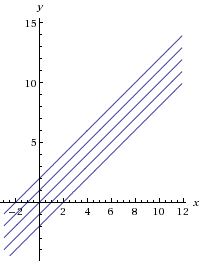
\includegraphics[scale=1]{fig/C2_S5_9}
\item[(10)]
Graph: \\
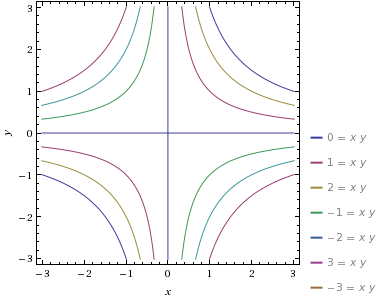
\includegraphics[scale=1]{fig/C2_S5_10}
\item[(11)]
$$\overline{0} + \overline{0} = \overline{1} + \overline{1} = \overline{0}$$
$$\overline{1} + \overline{0} = \overline{1}$$
$$\overline{0}\cdot\overline{0} = \overline{0}\cdot\overline{1} = \overline{0}$$
$$\overline{1}\cdot\overline{1} = \overline{1}$$
Note that the commutative, associative, and distributive properties of addition and multiplication hold as well.
\item[(12)]
Consider the coset $aN$ and the fiber of $\varphi$ on $a$, $\varphi^{-1}(a)$. Consider $g \in \varphi^{-1}(a)$, ie. $g$ is a member of the fiber of $\varphi$ on $a$. Then $\varphi(g) = \varphi(a)$. So $g \in aN$, and $\varphi^{-1}(a) \subseteq aN$. And, if $g \in aN$, then by definition $\varphi(g) = \varphi(a)$, so $g \in \varphi^{-1}(a)$. And $aN \subseteq \varphi^{-1}(a)$. Thus, $aN = \varphi^{-1}(a)$. Therefore the cosets are precisely the fibres of $\varphi$.
\end{itemize}
%\end{document}
\section{Cosets}
%\documentclass[12pt]{article}
%\usepackage{amsmath, amssymb, graphicx}
%\begin{document}
%\title{Chapter 2: Groups \\ Section 6: Cosets}
%\author{Alec Mouri}
%
%\maketitle
%\section*{Exercises}
\begin{itemize}
\item[(1)]
Consider $a \in \mathbb{Z}$, $hn \in n\mathbb{Z}$. Let $b = a + hn$. Using the division algorithm, we can write $a$ as $qn + r$, for $r < n$. So $b = (q + h)n + r$. Let $b_1 = (q_1 + h)n + r_1$, $b_2 = (q_2 + h)n + r_2$. $b_1, b_2$ are in the same coset if and only if $r_1 = r_2$. Since there are $n$ possible values of $r_1$ or $r_2$, then $[\mathbb{Z} : n\mathbb{Z}] = n$.
\item[(2)]
Consider the left cosets $aH$ and $bH$. Suppose for some $c$, $c \in aH$ and $c \in bH$. So $c = ah_1$ and $c = bh_2$, for $h_1, h_2 \in H$. So $ah_1 = bh_2 \rightarrow a = bh_2h_1^{-1}$. So $a \in bH$, ie. $a = bh_b = h_2h_1^{-1}$. So for $x \in aH$, then $x = ah_a = bh_2h_1^{-1}h_a \rightarrow x \in bH$. Thus, $aH \subseteq bH$. Similarly, $bH \subset aH$, so $aH = bH$. Thus, if $aH \neq bH$, then $aH \cap bH = \emptyset$.

Similarly, we can show all distinct right cosets do not overlap.
\item[(3)]
Suppose $G$ has order $p^n$, for $n \geq 1$. If $n = 1$, then $G$ is a cyclic group of order $p$, so for some $a$, $a$ generates $G$, and $a^p = 1$.

Suppose the statement is true for all $n \leq k - 1$. Then if $n = k$, for some $a \in G$, where $a \neq 1$, then $a$ generates some subgroup $H = \left\lbrace 1, a, a^2, ..., a^{x - 1} \right\rbrace$, where $x$ is the order of $a$. From the Counting Theorem, $|H|$ divides $|G|$, ie. $|H|$ is a power of $p$. If $|H| = p^n$, then $|a| = p^n$. So, $|a^{p^{n-1}}| = p$. If $|H| = p^i$, where $i < n$, then by the inductive hypothesis, the statement is true for $H$, and thus also for $G$.
\item[(4)]
Consider
$$H_1 = \begin{bmatrix}
a_1 & b_1 \\
c_1 & d_1
\end{bmatrix}, H_2 = \begin{bmatrix}
a_2 & b_2 \\
c_2 & d_2
\end{bmatrix} \in GL_2(\mathbb{R}), A = \begin{bmatrix}
i & i \\
& 1
\end{bmatrix} \in GL_2(\mathbb{C})$$
Then
$$H_1A = \begin{bmatrix}
a_1 & b_1 \\
c_1 & d_1
\end{bmatrix}\begin{bmatrix}
1 & i \\
& 1
\end{bmatrix} = \begin{bmatrix}
a_1 & b_1 + a_1i \\
c_1 & d_1 + c_1i
\end{bmatrix}$$
And
$$AH_2 = \begin{bmatrix}
1 & i \\
& 1
\end{bmatrix}\begin{bmatrix}
a_2 & b_2 \\
c_2 & d_2
\end{bmatrix} = \begin{bmatrix}
a_2 + c_2i & b_2 + d_2i \\
c_2 & d_2
\end{bmatrix}$$
For $c_2 \neq 0$, then $AH_2 \neq H_1A$. Thus the left and right cosets are different.
\item[(5)]
Since 3 and 5 are prime, then for some $h \neq 1 \in H$ and $k \neq 1 \in K$, then $H = \left\lbrace 1, h, h^2 \right\rbrace$, and $K = \left\lbrace 1, k, k^2, k^3, k^4 \right\rbrace$. Suppose for some $0 \leq i < 5$, $h = k^i$. Then $1 = k^{3i} \rightarrow i = 0 \rightarrow h = 1$, a contradiction The suppose for some $0 \leq j < 5$, then $h^2 = k^j$. Then $1 = k^{3j} \rightarrow j = 0 \rightarrow h^2 = 1$, a contradiction. So, $H \cap K = \left\lbrace 1 \right\rbrace$
\item[(6)]
From (5.13), the left cosets of $\text{ker }\varphi$ are the fibres of $\varphi$. Let $\tau$ map fibres of $\varphi$ onto $\text{im }$. Let $A, B \in \text{im }\varphi$, and $\varphi^{-1}(A), \varphi^{-1}(B)$ be fibres of $\varphi$ on $A$ and $B$ respectively, where $A \neq B$. That is, $\tau(\varphi^{-1}(A)) = A$, and $\tau(\varphi^{-1}(B)) = B$. For $a \in \varphi^{-1}(A), b \in \varphi^{-1}(B)$, then clearly $a \neq b$, and so $\varphi(a) = A, \varphi(b) = B$. So $\tau$ is injective. And since $\varphi$ is surjective onto $\text{im }\varphi$ by definition, then $\tau$ is surjective. Thus, $\tau$ is a bijection. So, $[G: \text{ker }G] = |\text{im }\varphi|$. Thus by the Counting Theorem, $|G| = |\text{ker }\varphi|[G: \text{ker }G] = |\text{ker }\varphi| \cdot |\text{im }\varphi|$.
\item[(7)]
\begin{itemize}
\item[(a)]
Let $a, b \in G$. Then $\varphi(ab) = (ab)^2 = a^2b^2 = \varphi(a)\varphi(b)$. So $\varphi$ is a homomorphism.

Let $H$ be the subgroup generated by $x$. Since $|H|$ divides $|G|$, and $|G|$ is odd, then $|x| = |H| = 2k + 1$ is odd. Let $\tau(x) = x^{k + 1}$. Then $\varphi(\tau(x)) = \tau(\varphi(x)) = x^{2(k+1)} = x$. So, $\varphi$ is a bijection. Thus, $\varphi$ is an automorphism.
\item[(b)]
Claim: Let $G$ be an abelian group. Consider $r$, where $gcd(r, |G|) = 1$, ie. $r$ is relatively prime to $|G|$. Then $\varphi(x) = x^r$ is an automorphism.

Let $a, b \in G$. Then $\varphi(ab) = (ab)^2 = a^2b^2 = \varphi(a)\varphi(b)$. So $\varphi$ is a homomorphism.

Let $H$ be the subgroup generated by $x$. Since $|H|$ divides $|G|$, and $|G|$ is relatively prime with $r$, then $|x| = |H|$ is also relatively prime with $r$. Write $1 = cr + d|H|$ for some $c, d$. Let $\tau(x) = x^{c}$. Then $\varphi(\tau(x)) = \tau(\varphi(x)) = x^{cr} = x^{1 - d|H|} = x$. So, $\varphi$ is a bijection. Thus, $\varphi$ is an automorphism.
\end{itemize}
\item[(8)]
Consider the coset $x+W$, where $Ax = B$. If $y \in x + W$, then $y = x+w$, where $w \in W$. Then $Ay = A(x+w) = Ax + Aw = B$. So, $y$ is a solution to $AX = B$.

Consider $y$ such that $Ay = B$. Then $B = B + 0 = Ay + Aw = A(y + w)$, where $w \in W$. So $y+w \in x+W$.

Therefore, the solutions of $AX = B$ forms a coset.

\item[(9)]
\begin{itemize}
\item[(a)]
Suppose $|G|$ is finite. Then $[G : H]$ is also finite. So there are a finite number of left cosets: $a_1H, a_2H, ..., a_nH$. Let $x \in a_iH \rightarrow x = a_ih$. Then $a_i^{-1}x = h \rightarrow x^{-1}a_i = h^{-1} \rightarrow x^{-1} = h^{-1}a_i \rightarrow x^{-1} \in Ha_i^{-1}$. So there is a 1:1 correspondence between $a_iH$ and $Ha_i^{-1}$. Thus there are $n$ right cosets.
\item[(b)]
Consider the cosets $aH$ and $Ha^{-1}$. Define $\varphi$ as $\varphi(aH) = Ha^{-1}$. Note that if $aH = bH$, then for $h_a, h_b \in H$, $ah_a = bh_b \rightarrow b^{-1}a \in H \rightarrow b^{-1}(a^{-1})^{-1} \in H \rightarrow b^{-1}(a^{-1})^{-1} = h_1h_2 \rightarrow h_1^{-1}b^{-1} = h_2a^{-1} \rightarrow Ha^{-1} = Hb^{-1}$. So $\varphi$ is well defined. Define $\varphi^{-1}(Ha) = a^{-1}H$ Note that $\varphi^{-1}(\varphi(aH)) = aH$, and $\varphi(\varphi^{-1}(Ha)) = Ha$, so there is a bijective correspondence between left and right cosets. Thus the number of left and right cosets are equal.
\end{itemize}
\item[(10)]
\begin{itemize}
\item[(a)]
Consider the two left cosets $aH$ and $bH$. I claim that $aH = Ha$, and $bH = Hb$. Suppose for $ah_1 \in aH$, that $ah_1 \in Hb$. Then for some $h_2$, $ah_1 = h_2b \rightarrow ah_1h_2^{-1} \in b$. So $b \in aH$. But $b \in bH$, and $aH \cap bH = \emptyset$ Thus, $ah_1 \not \in Hb$. Then $ah_1 \in Ha$. Similarly, for $h_1a \in Ha$, then $h_1a \in aH$. Thus, $aH = Ha$. We can similarly show that $bH = Hb$. Therefore, $H$ is normal.
\item[(b)]
Consider the subgroup $H = \left\lbrace 1, xy \right\rbrace$ of $S_3$. Then $H$ has index 3: the left cosets are $H = \left\lbrace 1, xy \right\rbrace, xH = \left\lbrace x, x^2y \right\rbrace, yH = \left\lbrace y, x^2y \right\rbrace$. But the right cosets are $H = \left\lbrace 1, xy \right\rbrace, Hx = \left\lbrace x, y \right\rbrace, Hx^2 = \left\lbrace x^2, x^2y \right\rbrace$. Since the left and right cosets do not correspond, then $H$ is not normal.
\end{itemize}
\item[(11)]
\begin{itemize}
\item[(a)]
If $G$ contains an element $x$ of order 6, then $G$ is	 a cyclic group generated by $x$.

Define $\varphi(x^n) = n \in 6\mathbb{Z}$. Then $\varphi(x) = 1$, so $\varphi$ is a homomorphism. And, let $\tau(n) = x^n$. Then $\varphi(\tau(n)) = 1$, and $\tau(\varphi(x^n)) = x^n$. So, $\varphi$ is a bijection, and is therefore an isomorphism. Thus, $G \simeq 6Z$
\item[(b)]
Suppose $G$ is abelian, ie. $xy = yx$. Let $x$ be of order 3. $y$ is of order $2$ or $3$. If $y$ is of order 3, then $J = \left\lbrace 1, y, y^2 \right\rbrace$ is a subgroup of $G$. Note that $y \in H$ (otherwise $H + J = \left\lbrace 1, x, x^2, y, y^2 \right\rbrace$, so $1 \neq a \not \in H + J$ has order 1, a contradiction), so $H = J$. Thus there exists some $y$ such that $y$ has order 2. Then $6$ is the order of $xy$, a contradiction. So $G$ is not abelian. 

Let $a$ have order 3 and $b$ have order 2. Then $\varphi(a^ib^j) = x^ib^j$. Thus is clearly an isomophism. Thus $G \simeq S_3$.
\item[(c)]
Suppose all elements of $G$ have order 1 or 2. Let $x, y \in G$. Then $(xy)^2 = y^2 = 1$. Then $xy = yx$. So $G$ is abelian. But, for distinct $x, y, z$, then $1, x, y, z, xy, yz, xz$ are all distinct. Thus $G$ does not exist.
\end{itemize}
\item[(12)]
Let 
$$A = \begin{bmatrix}
a_1 & a_2 \\
0 & 1
\end{bmatrix}$$
Then
$$AH = \begin{bmatrix}
a_1 & a_2 \\
0 & 1
\end{bmatrix}\begin{bmatrix}
x & 0 \\
0 & 1
\end{bmatrix} = \begin{bmatrix}
xa_1 & a_2 \\
0 & 1
\end{bmatrix}$$
And
$$HA = \begin{bmatrix}
x & 0 \\
0 & 1
\end{bmatrix}\begin{bmatrix}
a_1 & a_2 \\
0 & 1
\end{bmatrix} = \begin{bmatrix}
xa_1 & xa_2 \\
0 & 1
\end{bmatrix}$$
Left cosets: \\
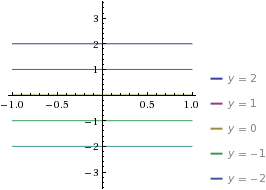
\includegraphics[scale=2.0]{fig/C2_S6_12-1} \\
Right cosets: \\
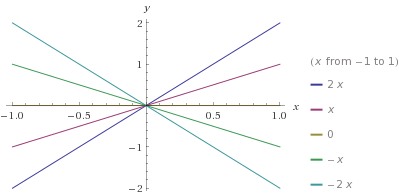
\includegraphics[scale=1.5]{fig/C2_S6_12-2}
\end{itemize}
%\end{document}
\section{Restriction of a Homomorphism to a Subgroup}
%\documentclass[12pt]{article}
%\usepackage{amsmath, amssymb, graphicx}
%\begin{document}
%\title{Chapter 2: Groups \\ Section 7: Restriction of a Subgroup to a Homomorphism}
%\author{Alec Mouri}
%
%\maketitle
%\section*{Exercises}
\begin{itemize}
\item[(1)]
$|\text{im }\varphi|$ divides both $G$ and $G'$, so since $|G|$ and $|G'|$ have no common factors, then $|\text{im }\varphi| = 1$. Since $\varphi(1) = 1$, then for all $x$, $\varphi(x) = 1$.
\item[(2)] Consider $S_4$. Consider
$$A = \begin{bmatrix}
& 1 \\
1 \\
& & 1 \\
& & & 1
\end{bmatrix}, B = \begin{bmatrix}
& 1 \\
1 \\
& & & 1 \\
& & 1
\end{bmatrix}$$
Note that $A^2 = B^2 = I_4$, and $\det A = -1$ and $\det B = 1$.
\item[(3)]
\begin{itemize}
\item[(a)]
First, consider $H$ to be a nontrivial subgroup. Then for some $x, y$, $xH \neq yH$. Then $xH \cap yH = \emptyset$.

Now consider arbitrary subgroups $H$ and $K$. Suppose $xH \cap yK$ is nonempty. Then there exists some $a \in xH \cap yK$, where for some $h \in H, k \in K$, $xh = yk$. So, $aH = xH$ and $aK = yK$. So $xH \cap yK = aH \cap aK$. So $z \in aH \cap aK \rightarrow z \in aH, aK \rightarrow a^{-1}z \in H \cap K \rightarrow z \in a(H \cap K)$.
\item[(b)]
Suppose $[G:H]$ and $[G:K]$ are finite. Then for $a \in G$, then $a(H \cap K) = aH \cap aK$. Since there are finite $aH$ and $aK$, then there is finite $aH \cap aK$. So $[G:H\cap K]$ is finite.
\end{itemize}
\item[(4)]
Let $a, b \in K \cap H$. Then $ab \in H$, and $ab \in K$, so $ab \in K \cap H$. And, $1 \in K \cap H$. And, if $a \in K \cap H$, then $a \in K$ and $a \in H$, so $a^{-1} \in K$ and $a^{-1} \in H$, so $a^{-1} \in K \cap H$. So, $K \cap H$ is a subgroup of both $H$ and $K$.

Suppose $K$ is a normal subgroup of $G$. Then for $g \in G, k \in K$, then $gkg^{-1} = k' \in K$. Consider $k' \in K \cap H$. Then for $a, h \in H$, $hk'h^{-1} \in H, K$. Thus, $H \cap K$ is a normal subgroup of $H$.
\item[(5)]
Let $x \in HN$. Then for $h \in H, n \in N$, $x = hn$. Suppose $hnh^{-1} = n'$, for some $n' \in N$. Then $n = h^{-1}n'h$, so $x = hh^{-1}n'h = n'h \rightarrow x \in NH$. So $HN \subseteq NH$. Similarly, $NH \subseteq HN$. So $HN = NH$. 

Let $h_1n_1, h_2n_2 \in HN$. Then for some $n' \in N, h' \in H$, $h_1n_1h_2n_2 = h_1h'n'n_2 \in HN$. And, $1 \in HN$. And, let $hn \in HN$. Note that $n^{-1}h^{-1} \in HN$, and $hnn^{-1}h^{-1} = 1$, so $(hn)^{-1} \in HN$. So $HN$ is a subgroup.
\item[(6)]
Let $kh \in KH$. Then $\varphi(kh) = \varphi(k)\varphi(h)$, so $kh \in \varphi^{-1}(\varphi(H))$. And, let $x \in \varphi^{-1}(\varphi(H))$. Then for some $h \in H$, $\varphi(x) = \varphi(h)$. For $k \in K$, $\varphi(x) = \varphi(kh) \rightarrow x \in KH$. Thus $KH = \varphi^{-1}(\varphi(H))$.
\item[(7)]
Consider two subgroups $A$ and $B$ of order 5. Since 5 is prime, then $A \cap B$ is either 1 or 5. Suppose there are at least 8 such subgroups. Suppose for any two subgroups $A, B$, $|A \cap B| = 1$, ie. $A \cap B = \left\lbrace 1 \right\rbrace$. Then $30 = |G| \geq 8(4) + 1 = 33$. Contradiction. So for some $A, B$, $A = B$. So, we must have at most 7 distinct subgroups of order 5.
\item[(8)]
Let $A, B \in G$, where $A \neq B$, and $A$ and $B$ contain $N$ Suppose for sake of contradiction that $\varphi(A) = \varphi(B)$. Without loss of generality assume that there exists some $a \in A$, and $a \not \in B$, so $a \not \in N$. Then $\varphi(ab) = \varphi(a)\varphi(b) \in \varphi(B)$. Then, for some $b' \in B$, $\varphi(a)\varphi(b) = \varphi(b')$. If $b \in N$, then $\varphi(a) = \varphi(b')$, so $a \in B$. Otherwise, then $1 = \varphi(b'b^{-1}a^{-1}) \rightarrow b'b^{-1}a^{-1} \in N \rightarrow a \in B$. This is a contradiction. Thus, $\varphi(A) \neq \varphi(B)$, so $\varphi$ is injective on subgroups of $G$. 

Consider $H' \leq G'$. For $h \in H'$, since $\varphi$ is surjective, then for some $g \in G$, $\varphi(g) = h$. Define $H = \left\lbrace g \in G : \varphi(g) \in H' \right\rbrace$. For $a, b \in H$, then $\varphi(ab) = \varphi(a)\varphi(b) \in H'$. And, $1 \in H$. And, $\varphi(a)^{-1} = \varphi(a^{-1}) \in H' \rightarrow a^{-1} \in H$. Thus, $H$ is a group. So $\varphi$ is surjective on subgroups of $G$.

Thus, $\varphi$ is a bijective correspondence.

Normal subgroups corresponding follows from Proposition 7.4.
\item[(9)]
$$G \leftrightarrow G', \left\lbrace 1, x^6 \right\rbrace \leftrightarrow \left\lbrace 1 \right\rbrace,$$
$$\left\lbrace 1, x^3, x^6, x^9 \right\rbrace \leftrightarrow \left\lbrace 1, y^3 \right\rbrace, \left\lbrace 1, x^2, x^4, x^6, x^8, x^{10} \right\rbrace \leftrightarrow \left\lbrace 1, y^2, y^4 \right\rbrace$$
\end{itemize}
%\end{document}
\section{Products of Groups}
%\documentclass[12pt]{article}
%\usepackage{amsmath}
%\begin{document}
%\title{Chapter 2: Groups \\ Section 8: Products of Groups}
%\author{Alec Mouri}
%
%\maketitle`
%\section*{Exercises}
\begin{itemize}
\item[(1)]
Let $(g, g') \in G \times G'$. There are $|G|$ possible values of $g$, and $|G'|$ possible values of $g'$. Then $|G \times G'| = |G||G'|$.
\item[(2)]
Consider $X = \left\lbrace 1, x, x^2 \right\rbrace$ and $Y = \left\lbrace 1, y \right\rbrace$. $X$ and $Y$ are nontrivial groups, and $S_3 = XY$.
\item[(3)]
Let $G$ be a finite cyclic group of order $rs$, and let $R$ and $S$ be cyclic groups of orders $r$ and $s$ respectively.

Suppose $G \simeq R \times S$. Then there exists an isomorphism $\varphi: G \mapsto R \times S$. Let $g \in G$ and $(a, b) \in R \times S$ such that $\varphi(g) = (a, b)$. Note that $|g| = |(a, b)|$. If $g$ generates $G$, then $|g| = |(a, b)| = rs \rightarrow (a^{rs}, b^{rs}) = 1$. Suppose $c = gcd(r, s) \neq 1$, so $r = cr'$ and $s = cs'$. So $(a, b)^{r's'c} = (a^{r's'c}, b^{r's'c}) = (a^{rs'}, b^{r's}) = (1, 1)$. But since $r's'c < rs$, then $|(a, b)| < rs$. So, $\varphi$ is not an isomorphism. By contradiction, $r, s$ have no common factor.

Suppose $r$ and $s$ have no common factors. Define $\varphi(g) = (a, b)$, where $a, b, g$ generate $R, S, G$ respectively. Then for $i < rs$, $\varphi(g^i) = (a, b)^i$. So $\varphi(g^ig^j) = \varphi(g^{i+j}) = (a, b)^{i + j} = (a, b)^i(a, b)^j$. So $\varphi$ is a homomorphism.

Suppose $g^i \neq g^j$, ie. $i \neq j$ where $i, j < rs$. If $\varphi(g^i) = \varphi(g^j)$, then $(a, b)^i = (a, b)^j \rightarrow a^i = a^j, b^i = b^j$. If $a^i = a^j$, then $r$ divides both $j - i$. Similarly, if $b^i = b^j$, then $s$ divides both $j - i$. But since $gcd(r, s) = 1$, then this implies $rs$ divides $j - i$. So if $j - i < rs$, then $j = i$. So, $\varphi$ is injective. And, for $m, n, c, d$ $(a^m, b^n) = (a^{cr + m}, b^{ds + n}) = (a^i, b^i) = \varphi(g^i)$ for some $i$. So $\varphi$ is surjective, and thus $\varphi$ is an isomorphism.
\item[(4)]
\begin{itemize}
\item[(a)]
Since $G$ is abelian, then $H$ and $K$ are normal. And, $H \cap K = \left\lbrace 1 \right\rbrace$. Consider $g \in G$. If $g > 0$, then for some $k \in K$, $g = k \rightarrow g \in HK$. If $g < 0$, then $g = -k \rightarrow g \in HK$. So $G = HK$. Thus, $G \simeq H \times K$.
\item[(b)]
Let
$$g = \begin{bmatrix}
a & b \\
& c
\end{bmatrix}, g^{-1} = \begin{bmatrix}
a^{-1} & -ba^{-1}c^{-1} \\
& c^{-1}
\end{bmatrix}, k = \begin{bmatrix}
1 & d \\
& 1
\end{bmatrix}$$
Then
$$gkg^{-1} = \begin{bmatrix}
a & b \\
& c
\end{bmatrix}\begin{bmatrix}
1 & d \\
& 1
\end{bmatrix}\begin{bmatrix}
a^{-1} & -ba^{-1}c^{-1} \\
& c^{-1}
\end{bmatrix}$$
$$= \begin{bmatrix}
a & b \\
& c
\end{bmatrix}\begin{bmatrix}
a^{-1} & dc^{-1} - ba^{-1}c^{-1} \\
& c^{-1}
\end{bmatrix} = \begin{bmatrix}
1 & adc^{-1} \\
& 1
\end{bmatrix} \in K$$
And, since $H$ is in the center of $G$, then $H$ is normal. And, $H \cap K = \left\lbrace I \right\rbrace$. And, for $g \in G$, $a \neq 0, b \neq 0$,
$$g = \begin{bmatrix}
a & b \\
& c
\end{bmatrix} = \begin{bmatrix}
a \\
& c
\end{bmatrix}\begin{bmatrix}
1 & a^{-1}b\\
& 1
\end{bmatrix} \in HK$$
So, $HK = G$. So, $G \simeq H \times K$.
\item[(c)]
Since $C^\times$ is abelian, then $H$ and $K$ are normal. And, $H \cap K = \left\lbrace 1 \right\rbrace$. Consider $a + bi \in C^\times$. Then 
$$a + bi = \left(\frac{a}{\sqrt{a^2+b^2}} + \frac{b}{\sqrt{a^2+b^2}}i\right)\frac{1}{a^2+b^2} \in HK$$
So, $HK = G$. So $G \simeq H \times K$.
\end{itemize}
\item[(5)]
Suppose $(g_1, g_2)$ generates $G_1 \times G_2$. Then for some $i$, $(g_1, g_2)^i = (1, g)$, where $g \neq 1$. Since $G_1$, $G_2$ are infinite cyclic, then for $g_1^i = 1$, then $i = 0 \rightarrow g = 1$. Since no generator then exists, then $G_1 \times G_2$ is not infinite cyclic.
\item[(6)]
Consider the two groups $A, B$. Let $(a, b) \in A \times B$ be part of the center of $A \times B$. Then for $(c, d) \in C \times D$, then $(c, d)(a, b) = (a, b)(c, d)$. Then $(ca, db) = (ac, bd) \rightarrow ca = ac, db = bd$, so $a$ is part of the center of $A$, and $b$ is part of the center of $B$. So, the center of $A \times B$ is part of the product of the centers of $A$ and $B$.

Let $a \in A$ and $b \in B$ be parts of the centers of $A$ and $B$. Then for $c \in A, d \in D$, $ac = ca$ and $bd = db$. Then $(a, b)(c, d) = (ac, bd) = (ca, db) = (c, d)(a, b)$, so $(a, b)$ is part of the center of $A \times B$.

Thus, the product of the centers of $A$ and $B$ is precisely the center of $A \times B$.
\item[(7)]
\begin{itemize}
\item[(a)]
Suppose $HK$ is a subgroup. Note for any $kh \in KH$, $(kh)^{-1} = h^{-1}k^{-1} \in HK$, so $KH \subseteq HK$. And, since for $h, k$, $(hk)^{-1} = k^{-1}h^{-1} \in KH$. So $HK \subseteq KH$. Then $HK = KH$.

Let $HK = KH$. Let $h_1, k_1, h_2k_2 \in HK$. First, note that $k_1h_2 = h_3k_3 \in HK$. Then $h_1k_1h_2k_2 = h_1h_3k_3k_2 \in HK$. And, clearly $1 \in HK$. And, for $hk \in HK$, note that $k^{-1}h^{-1} \in HK$, and $hkk^{-1}h^{-1} = 1$. So, $HK$ is a subgroup.
\item[(b)]
Consider the subgroups of $S_3$
$$A = \left\lbrace \begin{bmatrix}
1 \\
& 1 \\
& & 1
\end{bmatrix}, \begin{bmatrix}
& 1 \\
1 \\
& & 1
\end{bmatrix} \right\rbrace, B = \left\lbrace \begin{bmatrix}
1 \\
& 1 \\
& & 1
\end{bmatrix}, \begin{bmatrix}
1 \\
& & 1 \\
& 1
\end{bmatrix} \right\rbrace$$
Then
$$AB = \left\lbrace \begin{bmatrix}
1 \\
& 1 \\
& & 1
\end{bmatrix}, \begin{bmatrix}
& 1 \\
1 \\
& & 1
\end{bmatrix}, \begin{bmatrix}
1 \\
& & 1 \\
& 1
\end{bmatrix}, \begin{bmatrix}
& & 1 \\
1 \\
& 1
\end{bmatrix} \right\rbrace$$
But
$$BA = \left\lbrace \begin{bmatrix}
1 \\
& 1 \\
& & 1
\end{bmatrix}, \begin{bmatrix}
& 1 \\
1 \\
& & 1
\end{bmatrix}, \begin{bmatrix}
1 \\
& & 1 \\
& 1
\end{bmatrix}, \begin{bmatrix}
& 1 \\
& & 1 \\
1
\end{bmatrix} \right\rbrace$$
So $AB \neq BA$.
\end{itemize}
\item[(8)]
Let $A, B$ be normal subgroups of orders 3 and 5 respectively. Then $AB \leq G$. And, since $A \cap B = \left\lbrace 1 \right\rbrace$, then $AB$ is isomorphic to $A \times B$. Since $|(a, b)| = 15$, then $AB$ has an element that is order $15$.
\item[(9)]
Suppose $h_1k_1 = h_2k_2$. Then $h_2^{-1}h_1 = k_2k_1^{-1} \in H, K$. Since $H \cap K = \left\lbrace 1 \right\rbrace$, then $h_1 = h_2$ and $k_2 = k_1$. So, $|HK| = ab = |G|$, so $HK = G$.

Let $G = \left\lbrace 1, x, ..., x^7 \right\rbrace, H = \left\lbrace 1, x^4 \right\rbrace, K = \left\lbrace 1, x^2, x^4, x^6 \right\rbrace$. Since $H \times K$ has no elements of order 8, then $G$ is not isomorphic to $H \times K$.
\item[(10)]
Consider $(x, y)^k$. If $k = lcm(m ,n)$, then $(x, y)^k = (1, 1)$. Suppose $i < k$, where $(x, y)^i = (1, 1)$. Then $x^i = y^i = 1$. But $i$ is a multiple of $m$ and $n$, a contradiction since $k$ is the least such number by definition. Thus, $|(x, y)| = lcm(m, n)$
\item[(11)]
\begin{itemize}
\item[(a)]
Since $G$ is abelian, then $H$ and $K$ are normal. And, $H \cap K = \left\lbrace 1 \right\rbrace$. And, since $|H||K| = |G|$ and $HK \leq G$, then $HK = G$. Thus, $G$ is isomorphic to $H \times N$.
\item[(b)]
Since the left cosets of $N$ correspond to the fibres of $\varphi$, then for $g \in G$ we can write $g = hn$, where $h \in H, n \in N$. So, we can define $\tau(g) = (h, n)$. Clearly, $\tau$ is a bijection.

Consider $S_3$ and the subgroup $A = \left\lbrace 1, y \right\rbrace$, where $\varphi: S_3 \rightarrow S_3 \times A$ is a bijection:

$$\varphi(1) = (1, 1), \varphi(y) = (y, 1), \varphi(x) = (1, x),$$
$$\varphi(x^2) = (1, x^2), \varphi(yx) = (y, x), \varphi(yx^2) = (y, x^2)$$
And
$$\varphi(yxyx^2) = \varphi(yyx^2x^2) = \varphi(x) = (1, x)$$
But
$$\varphi(yx)\varphi(yx^2) = (y, x)(y, x^2) = (1, 1) \neq \varphi(x)$$
Thus $\varphi$ is not an isomorphism.
\end{itemize}
\end{itemize}
%\end{document}
\section{Modular Arithmetic}
%\documentclass[12pt]{article}
%\usepackage{amsmath, amssymb}
%\begin{document}
%\title{Chapter 2: Groups \\ Section 9: Modular Arithmetic}
%\author{Alec Mouri}
%
%\maketitle`
%\section*{Exercises}
\begin{itemize}
\item[(1)]
$$(7 + 14)(3 - 16)\equiv (21)(-13) \equiv (4)(4) \equiv 16 \mod 17$$
\item[(2)]
\begin{itemize}
\item[(a)]
$$0^2 \equiv 0 \mod 4$$
$$1^2 \equiv 1 \mod 4$$
$$2^2 \equiv 4 \equiv 0 \mod 4$$
$$3^2 \equiv 9 \equiv 1 \mod 4$$
So $a^2 \mod 4$ is always either 0 or 1.
\item[(b)]
$$0^2 \equiv 0 \mod 8$$
$$1^2 \equiv 1 \mod 8$$
$$2^2 \equiv 4 \mod 8$$
$$3^2 \equiv 9 \equiv 1 \mod 8$$
$$4^2 \equiv 16 \equiv 0 \mod 8$$
$$5^2 \equiv 25 \equiv 1 \mod 8$$
$$6^2 \equiv 36 \equiv 4 \mod 8$$
$$7^2 \equiv 49 \equiv 1 \mod 8$$
So $a^2 \mod 8$ is always either 0, 1, or 4.
\end{itemize}
\item[(3)]
\begin{itemize}
\item[(a)]
$$(0)(2) \equiv 0 \mod 6$$
$$(1)(2) \equiv 2 \mod 6$$
$$(2)(2) \equiv 4 \mod 6$$
$$(3)(2) \equiv 6 \equiv 0 \mod 6$$
$$(4)(2) \equiv 8 \equiv 2 \mod 6$$
$$(5)(2) \equiv 10 \equiv 4 \mod 6$$
So, $2$ has no inverse modulo 6.
\item[(b)]
Suppose $a$ is the inverse of 2 modulo $n$. Then for some $b \in \mathbb{Z}$,
$$1 = 2a + bn \rightarrow n = (1 - 2a)b^{-1}$$
Since $1 - 2a$ is not even, then $n$ is odd.
\end{itemize}
\item[(4)]
Note that $(10)^i \equiv 1^i \equiv 1 \mod 9$. So,
$$a = d_0 + 10d_1 + ... + 10^nd_n \equiv d_0 + d_1 + ... + d_n \mod 9$$
\item[(5)]
\begin{itemize}
\item[(a)]
$$x = 2^{-1}5 \equiv (5)(5) \equiv 7 \mod 9$$
\item[(b)]
$$2x \equiv 5$$ has no solution modulo 6, since the possible values of $2x$ are $0, 2, 4$ modulo 6.
\end{itemize}
\item[(6)]
For all $n$, $x + y \equiv 2$ has a solution: $x = y = 1$. Note if $n = 1$, then $0 \equiv 1 \equiv 2$ modulo $n$, so the statement is trivially true.

If $2x - 3y \equiv 3 \mod n$, then $2x - 3y - 3$ divides $n$. If $x = 0, y = -1$, then $2x - 3y - 3 = 0$. 0 divides all integers, so the statement has a solution for all $n$.
\item[(7)]
$$(\overline{a}\cdot\overline{b})\cdot\overline{c} = ((a + cn)(b + dn))(c + en)$$
$$= (a + cn)((b + dn)(c + en)) = \overline{a}\cdot(\overline{b}\cdot\overline{c})$$

$$\overline{a}\cdot\overline{b} = (a + cn)(b + dn) = (b + dn)(a + cn) = \overline{b}\cdot\overline{a}$$
\item[(8)]
From Proposition 2.6, $1 = an + bm$. Then
$$1 \equiv an + bm \mod m \rightarrow 1 \equiv an \mod m$$
Since $gcd(n, m) = 1$, then $n^{-1} \equiv a \mod m$.

Similarly, $m^{-1} \equiv b \mod n$.
\end{itemize}
%\end{document}
\section{Quotient Groups}
%\documentclass[12pt]{article}
%\usepackage{amsmath, amssymb}
%\begin{document}
%\title{Chapter 2: Groups \\ Section 10: Quotient Groups}
%\author{Alec Mouri}
%
%\maketitle`
%\section*{Exercises}
\begin{itemize}
\item[(1)]
Let
$$G = \begin{bmatrix}
b & c \\
& d
\end{bmatrix} \rightarrow G^{-1} = \begin{bmatrix}
1/b & -c/(bd) \\
& 1/d
\end{bmatrix}$$
\begin{itemize}
\item[(a)]
$$GAG^{-1} = \begin{bmatrix}
b & c \\
& d
\end{bmatrix}\begin{bmatrix}
1 & a_{12} \\
& a_{22}
\end{bmatrix}\begin{bmatrix}
1/b & -c/(bd) \\
& 1/d
\end{bmatrix}$$
$$= \begin{bmatrix}
b & c \\
& d
\end{bmatrix}\begin{bmatrix}
1/b & -c/(bd) + a_{12}/d \\
& a_{22}/d
\end{bmatrix} = \begin{bmatrix}
1 & -c/d + a_{12}b/d + ca_{22}/d \\
& a_{22}
\end{bmatrix}$$
So $a_{11} = 1$ describes a normal subgroup $H$ of $G$. Define
$$\varphi(B) = \varphi\left(\begin{bmatrix}
a_{11} & a_{12} \\
& a_{22}
\end{bmatrix}\right) = a_{11} \in \mathbb{R}^\times$$
Clearly, $\varphi$ is a surjective homomorphism, and $H = \text{ker }\varphi$. So, $G/H \simeq \mathbb{R}^\times$.
\item[(b)]
$$GAG^{-1} = \begin{bmatrix}
b & c \\
& d
\end{bmatrix}\begin{bmatrix}
a_{11} & \\
& a_{22}
\end{bmatrix}\begin{bmatrix}
1/b & -c/(bd) \\
& 1/d
\end{bmatrix}$$
$$= \begin{bmatrix}
b & c \\
& d
\end{bmatrix}\begin{bmatrix}
a_{11}/b & -a_{11}c/(bd) \\
& a_{22}/d
\end{bmatrix} = \begin{bmatrix}
a_{11} & -a_{11}c/d + a_{22}c/d \\
& a_{22}
\end{bmatrix}$$
So if $a_{11} = 1, a_{22} = 2$, $c = d$, then
$$GAG^{-1} = \begin{bmatrix}
1 & 1 \\
& 2
\end{bmatrix} \not \in H$$
So, $a_{12} = 0$ does not describe a normal subgroup of $G$.
\item[(c)]
$$GAG^{-1} = \begin{bmatrix}
b & c \\
& d
\end{bmatrix}\begin{bmatrix}
a_{11} & a_{12} \\
& a_{11}
\end{bmatrix}\begin{bmatrix}
1/b & -c/(bd) \\
& 1/d
\end{bmatrix}$$
$$= \begin{bmatrix}
b & c \\
& d
\end{bmatrix}\begin{bmatrix}
a_{11}/b & -ca_{11}/(bd) + a_{12}/d \\
& a_{11}/d
\end{bmatrix} = \begin{bmatrix}
a_{11} & a_{12}b/d \\
& a_{11}
\end{bmatrix}$$
So $a_{11} = a_{22}$ defines a subgroup $H$ of $G$. Define
$$\varphi\left( \begin{bmatrix}
a_{11} & a_{12} \\
& a_{22}
\end{bmatrix}\right) = a_{11}a_{22}^{-1} \in \mathbb{R}^\times$$
Clearly, $\varphi$ is a surjective homomorphism, and $H = \text{ker }\varphi$. So, $G/H \simeq \mathbb{R}^\times$.
\item[(d)]
$$GAG^{-1} = \begin{bmatrix}
b & c \\
& d
\end{bmatrix}\begin{bmatrix}
1 & a_{12} \\
& 1
\end{bmatrix}\begin{bmatrix}
1/b & -c/(bd) \\
& 1/d
\end{bmatrix}$$
$$\begin{bmatrix}
b & c \\
& d
\end{bmatrix}\begin{bmatrix}
1/b & -c/(bd) + a_{12}/d \\
& 1/d
\end{bmatrix} = \begin{bmatrix}
1 & -c/d + ba_{12}/d + c/d \\
& 1
\end{bmatrix}$$
So $a_{11} = a_{22} = 1$ describes a normal subgroup $H$ of $G$. Define
$$\varphi\left( \begin{bmatrix}
a_{11} & a_{12}\\
& a_{22}
\end{bmatrix}\right) = (a_{11}, a_{22}) \in \mathbb{R}^\times \times  \mathbb{R}^\times$$
Clearly, $\varphi$ is a surjective homomorphism, and $H = \text{ker }\varphi$. So, $G/H \simeq \mathbb{R}^\times \times \mathbb{R}^\times$.
\end{itemize}
\item[(2)]
Let $an_1 \in aN, bn_2 \in bN$. Note first that for some $n_3 \in N$, $n_1b = bn_3$, since $N$ is normal. Then
$$an_1bn_2 = abn_3n_2 \in abN$$
And, let $abn \in abN$. Note that for some $m \in N$, $bn = mb$. So,
$$abn = amb = amb1 \in (aN)(bN)$$
So, $(aN)(bN) = abN$.
\item[(3)]
Consider $AN = B$. Since $a \in AN$, and $a \in NA$, then $AN = NA$. So, $N$ is normal, and since $A$ is arbitrary, and the cosets of $N$ form a partition, then the cosets of $N$ is clearly $P$.
\item[(4)]
\begin{itemize}
\item[(a)]
$$(1H)(xH) = \left\lbrace x, x^2, xy, x^2y \right\rbrace$$
$$(1H)(x^2H) = \left\lbrace x, x^2, xy, x^2y \right\rbrace$$
Note that $xy \in xH$, but $xH = \left\lbrace x, xy \right\rbrace$, so $(1H)(xH)$ and $(1H)(x^2H)$ are not cosets.
\item[(b)]
Let $G$ be a cyclic group of order 6 with generator $g$. Let $x = g^2$ and $y = g^3$. Then $x^3 = 1, y^2 = 1, xy = yx$. And, $g = x^2y, g^4 = x^2, g^5 = xy$, so $x, y$ generate $G$.
\item[(c)]
$$(1H)(xH) = \left\lbrace x, xy \right\rbrace = xH$$
$$(1H)(x^2H) = \left\lbrace x^2, x^2y \right\rbrace = x^2H$$
The generators from part b) describe an abelian group, so $H$ is a normal subgroup, whereas in part (a) $H$ was not a normal subgroup, so 10.1 did not hold.
\end{itemize}
\item[(5)]
Define $\varphi(a) = \text{sgn }a$. Clearly, $\varphi$ is a surjective homomorphism. And, $P = \text{ker }\varphi$. So, $\mathbb{R}^\times \simeq \text{sgn }a$.
\item[(6)]
$$(a + bi)H = \left\lbrace a+bi, -a-bi, -b + ai, b - ai \right\rbrace$$
Note that $(a+bi)H = (-a-bi)H = (-b+ai)H = (b-ai)H$.

Define 
$$\varphi(a + bi) = (a+bi)^4$$
Clearly, $\varphi$ is a surjective homomorphism. And, $\text{ker }\varphi = H$. So, $G/H \simeq G$.
\item[(7)]
All subgroups of $H$ are normal: let $N$ be a subgroup of $H$. Then for $h \in H$, $n \in N$,
$$hnh^{-1} = h(-h^{-1}n) = -hh^{-1}n = -n = n^{-1} \in N$$
If $N = H$ or $N = \left\lbrace 1 \right\rbrace$, then $N/H = N$.

Let $N = \left\lbrace 1, -1 \right\rbrace$. Define $\varphi(\pm i) = (1, -1), \varphi(\pm j) = (-1, 1), \varphi(\pm k) = (-1, -1), \varphi(\pm 1) = (1, 1)$. Clearly, $\varphi$ is surjective onto $(\pm 1, \pm 1) \simeq V_4$. And, $\varphi(ab) = \varphi(a)\varphi(b)$, so $\varphi$ is a homomorphism. And, $\text{ker }\varphi = N$. Thus, $H/N \simeq V_4$.

Let $N = \left\lbrace 1, -1, i, -i \right\rbrace$. Define $\varphi(a)$ as folllows: if $a \in N$, then $\varphi(a) = 1$, otherwise $\varphi(a) = -1$. If $a, b \in N$ or $a, b \not \in N$, then $\varphi(ab) = 1$. Otherwise, $\varphi(ab) = -1$. So $\varphi$ is an isomorphism, and is surjective onto $\left\lbrace 1, -1 \right\rbrace$. And, $\text{ker }\varphi = N$. Thus, $H/N \simeq \left\lbrace 1, -1 \right\rbrace$.
\item[(8)]
Let $g \in G, h \in H$. Then $\det(ghg^{-1}) = \det(g)\det(h)\det(g^{-1}) = \det(h)\det(g)\det(g)^{-1} = \det{h} > 0$. So, $H$ is a normal subgroup.

Define $\varphi(g) = \text{sgn}(\det(g))$. For $a, b \in G$, then $\varphi(ab) = \text{sgn}(\det(ab)) = \text{sgn}(\det(a)\det(b)) = \text{sgn}(\det(a))\text{sgn}(\det(b)) = \varphi(a)\varphi(b)$. So $\varphi$ is a homomorphism, and it is surjective onto $\left\lbrace 1, -1 \right\rbrace$. And, $\text{ker }\varphi = H$. Thus, $G/H \simeq \left\lbrace 1, -1 \right\rbrace$.
\item[(9)]
Let $(g, g') \in G \times G'$, and $(h, 1) \in G \times 1$. Then $(g, g')(h, 1)(g, g')^{-1} = (ghg^{-1}, 1) \in G \times 1$. So $G \times 1$ is a normal subgroup of $G \times G'$. And, define $\varphi((h, 1)) = h$. Clearly, $\varphi$ is a bijection, and $\varphi((h_1, 1)(h_2, 1)) = \varphi((h_1h_2, 1)) = h_1h_2 = \varphi((h_1, 1))\varphi((h_2, 1))$. So, $G \times 1 \simeq G$. And, define $\tau((g, g')) = g'$. Clearly, $\tau$ is surjective. And, $\tau((g_1, g_1')(g_2, g_2')) = \tau((g_1g_2, g_1'g_2')) = g_1'g_2' = \tau((g_1, g_1'))\tau((g_2, g_2'))$. And, $\text{ker }\tau = G \times 1$. Thus, $(G \times G')/(G \times 1) \simeq G'$.
\item[(10)]
Define $\varphi(a + bi) = \frac{1}{\sqrt{a^2+b^2}}(a + bi)$. Then for $a + bi, c = di$,
$$\varphi((a+bi)(c+di)) = \varphi(ac - bd + (ad + bc)i)$$
$$ = \frac{ac - bd + (ad + bc)i}{\sqrt{(ac - bd)^2 + (ad + bc)^2}} = \frac{ac - bd + (ad + bc)i}{\sqrt{a^2c^2 + b^2d^2 + a^2d^2 + b^2c^2}}$$
$$ = \frac{(a + bi)(c + di)}{\sqrt{(a^2 + b^2)(c^2+d^2)}} = \varphi(a+bi)\varphi(c+di)$$
So, $\varphi$ is a homomorphism, and it is surjective onto $U$. And, $\text{ker }\varphi = P$. So, $\mathbb{C}^\times/P \simeq U$.

Define $\tau(a+bi) = \sqrt{a^2 + b^2}$. Then for $a+bi, c+di$,
$$\tau((a+bi)(c+di)) = \tau(ac - bd + (ad + bc)i)$$
$$= \sqrt{(ac - bd)^2 + (ad + bc)^2} = \sqrt{a^2c^2 + b^2d^2 + a^2d^2 + b^2c^2}$$
$$= \sqrt{(a^2+b^2)(c^2+d^2} = \tau(a+bi)\tau(c+di)$$
So, $\tau$ is a homomorphism, and it is surjective onto $P^+$, the subgroup of positive reals. And, $\text{ker }\varphi = U$. So, $\mathbb{C}^\times/P \simeq P^+$.
\item[(11)]
Let $a = p + r$, where $p \in \mathbb{Z}$, and $0 \leq r < 1$. Define $\varphi(a) = r$. Then for $a_1 = p_1 + r_1, a_2 = p_2 + r_2 \in \mathbb{R}$, with $r_1 + r_2 = p_3 + r_3$. Then
$$\varphi(a_1 + a_2) = \varphi(p_1 + r_1 + p_2 + r_2)$$
$$= \varphi((p_1 + p_2 + p_3) + r_3) = r_3 = \varphi(a_1) + \varphi(a_2)$$
So $\varphi$ is a homomorphism, and it is surjective onto $[0, 1]$. And, $\text{ker }\varphi = \mathbb{Z}^+$. So, $\mathbb{R}^+/\mathbb{Z}^+ \simeq [0, 1)$ modulo 1.

Let $a = 2\pi p + r$, where $p \in \mathbb{Z}$, and $0 \leq r < 2\pi$. Define $\varphi(a) = r$. Then for $a_1 = 2 \pi p_1 + r_1, a_2 = 2\pi p_2 + r_2 \in \mathbb{R}$, with $r_1 + r_2 = 2\pi p_3 + r_3$. Then
$$\varphi(a_1 + a_2) = \varphi(2\pi p_1 + r_1 + 2\pi p_2 + r_2)$$
$$= \varphi(2\pi(p_1 + p_2 + p_3) + r_3) = r_3 = \varphi(a_1) + \varphi(a_2)$$
So $\varphi$ is a homomorphism, and it is surjective onto $[0, 2\pi]$. And, $\text{ker }\varphi = \mathbb{Z}^+$. So, $\mathbb{R}^+/2\pi\mathbb{Z}^+ \simeq [0, 2\pi)$ modulo $2\pi$.

Let $a \in [0, 1)$ modulo 1. Define $f(a) = 2\pi a \in [0, 2\pi)$ modulo $2\pi$. Clearly, $f$ is a bijection and is an isomorphism. So, $\mathbb{R}^+/\mathbb{Z}^+ \simeq \mathbb{R}^+/2\pi\mathbb{Z}^+$.
\end{itemize}
%\end{document}
\section{Miscellaneous Problems}
%\documentclass[12pt]{article}
%\usepackage{amsmath, amssymb}
%\begin{document}
%\title{Chapter 2: Groups \\ Miscellaneous Problems}
%\author{Alec Mouri}
%
%\maketitle
%\section*{Exercises}
\begin{itemize}
\item[(1)]
$$\prod_{j = 0}^{m-1} e^{\frac{j2\pi}{m}i} = e^{\frac{2\pi}{m}i\left(\sum_{j=0}^{m-1}j\right)} = e^{\pi(m-1)i} = (e^{\pi i})^{m-1} = (-1)^{m-1}$$
\item[(2)]
For all automorphisms $f$, $f(1) = 1$ and $f(-1) = -1$. And, if $f(i) = a$, then $f(-i) = -a$. So, each automorphism $f$ can be described by $f(i)$ and $f(j)$: there are 6 possibilities for $f(i)$, and given $f(i)$ there are 4 possibilities for $f(j)$. With these facts, it is trivial to compute $Aut(Q_8)$.
\item[(3)]
Let $|G| = 2n$. For $a \in G$, if $|a| \neq 2$, then either $a = 1$, or $a \neq a^{-1}$. Counting these elements, there is an odd number of elements. Therefore, there must be at least one element of order 2.
\item[(4)]
$$G = |H|[G : H], G = |K|[G : K] \rightarrow |H|[G : H] = |K|[G : K]$$
$$|H| = |K|[H : K] \rightarrow |K|[H : K][G : H] = |K|[G : K]$$
$$\rightarrow [G : K] = [G : H][H : K]$$
\item[(5)]
$\varphi: S \rightarrow T$ is an isomorphism of semigroups if for $a, b \in S$, $\varphi(ab) = \varphi(a)\varphi(b)$, and $\varphi$ is a bijection.

If $|S| = \infty$, and $s$ generates $S$, then $S \simeq (\mathbb{Z}^+ \geq 0)$, that is the additive semigroup of positive integers, that is described by the map $\varphi(s) = 1$.

If $|S| = n < \infty$, and $s$ generates $S$, then for some $0 \leq k < n$, then $s^n = s^k$. Then $\left\lbrace s^k, ..., s^{n-1} \right\rbrace$ forms a cyclic subgroup.
\item[(6)]
Since $S$ satisfies the Cancellation Laws, then for $a, b, c \in S$, if $ab = ac$, then $b = c$. Therefore, for some $x \in S, ax = 1 \rightarrow a, x$ have inverses. Therefore, $S$ is a group.
\item[(7)]
\begin{itemize}
\item[(a)]
Note that the path from $a$ onto itself is $f(t) = a \forall t$, so $a \simeq a$.

If $a \sim b$, then $f(t)$ is a path joining $a$ and $b$. Then $g(t) = f(1 - t)$ is a path joining $b$ and $a$. So, $b \sim a$.

If $a \sim b$ and $b \sim c$, then $f(t)$ is a path joining $a$ and $b$, and $g(t)$ is a path joining $b$ and $c$. Define $h(t)$ as follows: If $t \in [0, 1/2]$, then $h(t) = f(2t)$. If $t \in [1/2, 1]$, then $h(t) = g(2t - 1)$. Since for all $t$, $h(t) \in S$, then $a \sim c$.
\item[(b)]
Since $\sim$ is an equivalence relation on $S$, then $\sim$ partitions $S$. Since a subset $S$ is path connected if all points in $S$ follow $\sim$, then by definition $S$ is partitioned by path connected subsets.
\item[(c)]
$\left\lbrace x^2 + y^2 = 1 \right\rbrace, \left\lbrace xy = 0 \right\rbrace$ are path connected since they are continuous loci. $\left\lbrace xy = 1 \right\rbrace$ is not continuous at $x = 0$ or $y = 0$, so it is not path connected.
\end{itemize}
\item[(8)]
\begin{itemize}
\item[(a)]
Note that $AC, BD \in G$. Let $f(t)$ be the path from $A$ to $B$, and $g(t)$ be the path from $C$ to $D$. Then $f(0)g(0) = AC$, and $f(1)g(1) = BD$. And, $f(t)g(t) \in G$. So, $f(t)g(t)$ is a path from $AC$ to $BD$.
\item[(b)]
Let $A \in G$ where there is a path from $A$ to $I$. Then for $B \in G$, there is a path from $BA$ to $B$. So, there is a path from $BAB^{-1}$ to $BB^{-1} = I$. So, therefore the set of matrices connected to $I$ forms a connected component.
\end{itemize}
\item[(9)]
\begin{itemize}
\item[(a)]
Let $E$ be an elementary matrix of the first kind, where $e_{ij} = a, i \neq j$. Note that $E \in SL_n(\mathbb{R})$. And, there is a path $f(t)$ in $SL_n(\mathbb{R})$ from $E$ to $I$ defined as an operation on $e_{ij}$: $e_{ij}(t) = (1 - t)a$. For $A \in SL_n(\mathbb{R})$, then there is a path from $A$ to $I$. Thus $SL_n(\mathbb{R})$ is path connected.
\item[(b)]
Let $E$ be an elementary matrix of the third kind, where $e_{ii} = a$. There is a path $f(t)$ from $E$ to $I$ defined as an operation on $e_{ii}$: $e_{ii}(t) = 1 + (1 - t)(a - 1)$. So, elementary matrices of the third kind is a path connected subset.

So, for $A \in GL_n(\mathbb{R})$, since $A$ can be written as a product of elementary matrices of the first and third kinds, there is a path from $A$ to $I$ within the union of the elementary matrices of the first and third kinds.
\end{itemize}
\item[(10)]
\begin{itemize}
\item[(a)]
For $g \in G$, then for some $x$, $x = hgk \rightarrow h^{-1}xk^{-1} = g \in HgK$. So, $g$ is contained in some double coset. So the double cosets of $G$ covers all of $G$.

Suppose $x \in G$ is contained in $Hg_1K$ and $Hg_2K$. So, for some $h_1, h_2 \in H, k_1, k_2 \in K$, we have $h_1g_1k_1 = h_2g_2k_2 \rightarrow h_2^{-1}h_1g_1k_1k_2^{-1} = g_2 \in Hg_1K \rightarrow Hg_2K \subseteq Hg_1K$. Similarly, $g_1 \in Hg_2K \rightarrow Hg_1K \subseteq Hg_2K$. So, $Hg_1K = Hg_2K$. So, the double cosets are disjoint, and therefore partition $G$.
\item[(b)]
Consider $S_3$. Let $A = \left\lbrace 1, y \right\rbrace$ and $B = \left\lbrace 1, xy \right\rbrace$ be subgroups of $S_3$. Then
$$BA = \left\lbrace 1, x, xy, y \right\rbrace$$
But
$$Bx^2A = \left\lbrace x^2, x^2y \right\rbrace$$
So, not all double cosets have the same order.
\end{itemize}
\item[(11)]
Suppose $H$ is normal. Then for $h_1, h_2, h_3 \in H$, then $h_1g = gh_3$, so $h_1gh_2 = gh_3h_2 \in gH$. So, $HgH \subseteq gH$. Similarly, $gh_4 = gh_2h_3 = h_1gh_3$, so $gH \subseteq HgH$. Thus, $HgH = gH$.

Suppose $H$ is not normal. Clearly, $gH \in HgH$. And, there must exist some $h_1 \in H$ such that for some other $h_2 \in H$, $h_1gh_2 \not \in gH$: otherwise $H$ is normal. Thus $gH$ is a proper subset of $HgH$.
\item[(12)]
Let $A \in GL_n(\mathbb{R})$. Since $A$ is invertible, then $A$ can be written as $LPU$, where $L$ is a lower triangular matrix, $P$ is a permutation matrix, and $U$ is a upper triangular matrix with diagonal entries all 1. Then, for $B \in H, C \in K$, then
$$BAC = BLPUC \in HPK$$
\end{itemize}
%\end{document}

\chapter{Vector Spaces}
\section*{Exercises}
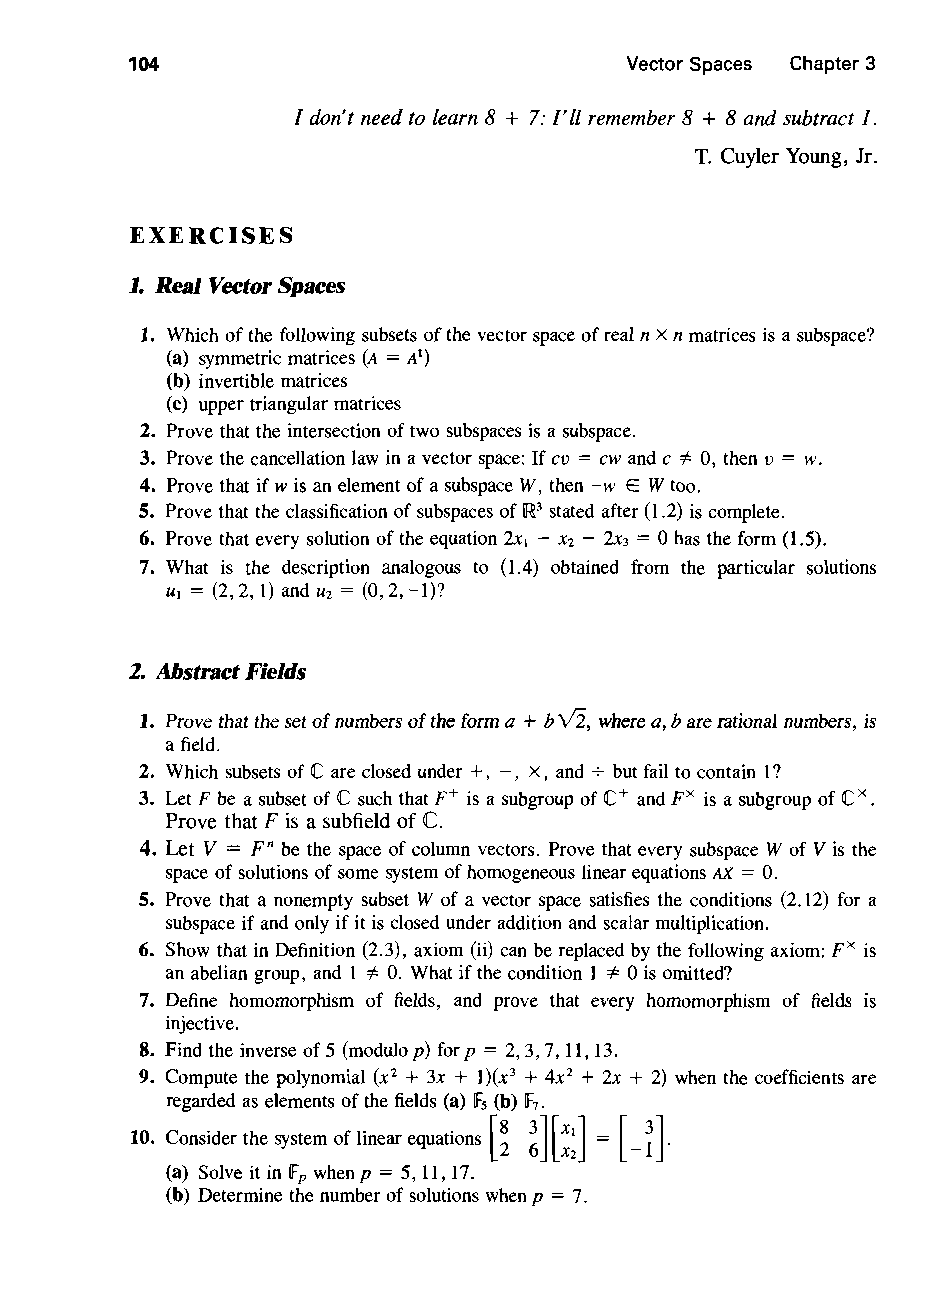
\includepdf[pages={1-},scale=0.85]{Exercises/C3_selection.pdf}
\section{Real Vector Spaces}
%\documentclass[12pt]{article}
%\usepackage{amsmath, amssymb}
%\begin{document}
%\title{Chapter 3: Vector Spaces \\ Section 1: Real Vector Spaces}
%\author{Alec Mouri}
%
%\maketitle
%\section*{Exercises}
\begin{itemize}
\item[(1)]
\begin{itemize}
\item[(a)]
Let $A, B$ be symmetric matrices. Then, $A + B = (A + B)^\top$. And, for $c \in \mathbb{R}$, $cA = cA^\top$. So, addition and scalar multiplication are closed rules of composition. So the symmetric matrices form a subspace.
\item[(b)]
The invertible matrices do not form a subspace. Consider
$$A = \begin{bmatrix}
1 \\
& 1
\end{bmatrix}, B = \begin{bmatrix}
& 1 \\
1
\end{bmatrix}$$
Then $\det(A + B) = 0$, so $A + B$ is not invertible.
\item[(c)]
Let $A, B$ be upper triangular matrices. Then, $A + B$ is also upper triangular. And, for $c \in \mathbb{R}$, $cA$ is also upper triangular. So, addition and scalar multiplication are closed rules of composition. So the upper triangular matrices form a subspace.
\end{itemize}
\item[(2)]
Consider the subspaces $\mathcal{A}, \mathcal{B}$. If $a, b \in \mathcal{A} \cap \mathcal{B}$, then $a + b \in \mathcal{A}$ and $a + b \in \mathcal{B}$, so $a + b \in \mathcal{A} \cap \mathcal{B}$. And, for $c \in \mathbb{R}$, similarly $ca \in \mathcal{A}$, and $cb \in \mathcal{B}$. So, $\mathcal{A} \cap \mathcal{B}$ is a subspace.
\item[(3)]
Let $cv = cw, c \neq 0$. Then $cv - cw = 0 \rightarrow c(v - w) = 0 \rightarrow v - w = 0 \rightarrow v = w$.
\item[(4)]
If $W$ is a subspace, then $W^+$ forms an abelian group. So, if $w \in W$, then necessairly $-w \in W$.
\item[(5)]
Clearly, the zero vector forms a subspace of $\mathbb{R}^3$.

Let $(x_1, y_1, z_1), (cx_1, cy_1, cz_1) \in \mathbb{R}^3$ be collinear passing through the origin. Then $(x_1, y_1, z_1) + (cx_1, cy_1, cz_1) = ((c + 1)x_1, (c + 1)y_1, (c + 1)z_1)$ lies on the same line. And, for $d \in \mathbb{R}^3$, $(dx_1, dy_1, dz_1)$ is also collinear.

Let $v_1 = (x_1, y_1, z_1), v_2 = (x_2, y_2, z_2) \in \mathbb{R}^3$ that are not collinear. Then $v_1, v_2$ is coplanar to some plane. Clearly, $(x_1, y_1, z_1) + (x_2, y_2, z_2)$ also lies in the same plane. And, for $d \in \mathbb{R}^3$, $(dx_1, dy_1, dz_1)$ is also coplanar.

And, clearly $\mathbb{R}^3$ is a subspace of itself: any three vectors that are not coplanar to each other forms $\mathbb{R}^3$.
\item[(6)]
Let $(x_1, x_2, x_3)$ be a solution. Then, $2x_1 - x_2 - 2x_3 = 0 \rightarrow x_1 = x_2/2 + x_3$. So, the solution has the form $(x_2/2 + x_3, x_2, x_3)$. And, letting $x_2/2 = y_2$. Then, the solution has the form $(y_2 + x_3, 2y_2, x_3)$.
\item[(7)]
Every solution has the form
$$c_1u_1 + c_2u_2 = \begin{bmatrix}
2c_1 \\
2c_1 + 2c_2 \\
c_1 - c_2
\end{bmatrix}$$
where $c_1, c_2$ are arbitrary constants.
\end{itemize}
%\end{document}
\section{Abstract Fields}
%\documentclass[12pt]{article}
%\usepackage{amsmath, amssymb}
%\begin{document}
%\title{Chapter 3: Vector Spaces \\ Section 2: Abstract Fields}
%\author{Alec Mouri}
%
%\maketitle
%\section*{Exercises}
\begin{itemize}
\item[(1)]
Let $a_1 + b_1\sqrt{2}, a_2 + b_2\sqrt{2} \in F$. Then:
$$a_1 + b_1\sqrt{2} + a_2 + b_2\sqrt{2} = (a_1 + a_2) + (b_1 + b_2)\sqrt{2} \in F$$
$$-(a_1 + b_1\sqrt{2}) = -a_1 + (-b_1)\sqrt{2} \in F$$
$$(a_1 + b_1\sqrt{2})(a_2 + b_2\sqrt{2}) = a_1a_2 + 2b_1b_2 + (a_1b_2 + a_2b_1)\sqrt{2} \in F$$
$$1 \in F$$
$$\left(a_1 + b_1\sqrt{2}\right)\left(\frac{a_1}{a_1^2 - 2b_1^2} - \frac{b_1}{a_1^2 - 2b_1^2}\sqrt{2}\right)$$
$$=\frac{a_1^2}{a_1^2 - 2b_1^2} - \frac{2b_1^2}{a_1^2 - 2b_1^2} + \frac{a_1b_1}{a_1^2 - 2b_1^2}\sqrt{2} - \frac{a_1b_1}{a_1^2 - 2b_1^2}\sqrt{2} = 1$$
$$\rightarrow (a_1 + b_1\sqrt{2})^{-1} \in F$$
Thus, $F$ is a field.
\item[(2)]
There is no such subset. If a subset $S$ is closed under division, then if $a \in S$, then $a^{-1} \in S$. But then $aa^{-1} = 1 \in S$. So, $S$ must contain 1.
\item[(3)]
Since $F^+$ is a subgroup of $\mathbb{C}^+$, then $F^+$ is abelian.

Since $F^\times$ is a subgroup of $\mathbb{C}^\times$, then $F^\times$ is abelian.

Let $a_1 + b_1i, a_2 + b_2i, a_3 + b_3i \in F$. Then
$$(a_1 + b_1i + a_2 + b_2i)(a_3 + b_3i) = ((a_1 + a_2) + (b_1 + b_2)i)(a_3 + b_3i)$$
$$= (a_1+ a_2)a_3 - (b_1 + b_2)b_3 + ((a_1 +a_2)b_3 + (b_1 + b_2)a_3)i$$
$$= a_1a_3 + a_2a_3 - b_1b_3 - b_2b_3 + (a_1b_3 + a_2b_3 + a_3b_1 + a_3b_2)i$$
$$= (a_1 + b_1i)(a_3 + b_3i) + (a_2 + b_2i)(a_3 + b_3i)$$
Thus, the distributive law holds, and $F$ is a subfield of $\mathbb{C}$.
\item[(4)]
Let $w \in W$, and $v \in V$, where $v \not \in W$. Note for all $x \in V$, we can write $x$ as $x = w + v$, for any $w, v$. Then, define $\varphi(x) = \varphi(v + w) = w$. That is, $\varphi(x)$ is the projection of $x$ onto $W$. Since $W$ is the kernel of $\varphi$, then there exists some $A$ such that $W$ is the solution set of $Ax = 0$.
\item[(5)]
Suppose $W$ is a subspace by 2.12. By (a) and (b), $W$ is closed under addition and scalar multiplication.

Suppose $W$ is closed under addition and scalar multiplication. Then, for $w, w' \in W, w + w' \in W$, and for $c \in F$, then $cw \in W$. And, $(-1)w = -w \in W$. So, $0 = w - w \in W$. Thus, $W$ is a subspace.
\item[(6)]
Since multiplication is associative and commutative, then $F^\times$ is abelian. Since $F^\times$ is a group, then it contains an identity: 1.

If $F^\times$ is abelian, then multiplication is associative and commutative. And, since $F^\times$ does not contain 0, then $0 \neq 1$.

Suppose 0 = 1. Then, $1 = 0 = 0 + 0 = 1 + 1$. This would mean that the real numbers are not a field.
\item[(7)]
A homomorphism $\varphi$ from a vector space $V$ to a vector space $V'$ both over the same field $F$ is a map $\varphi: V \rightarrow V'$ satisfying, for $v, v' \in V, c \in F$:
$$\varphi(v + v') = \varphi(v) + \varphi(v'), \varphi(vv') = \varphi(v)\varphi(v')$$
Suppose for $v \neq u$, $\varphi(v) = \varphi(u)$. Then $\varphi(v - u) = \varphi(v) - \varphi(u) = 0$. So, $\varphi((v - u)(v - u)^{-1}) = \varphi(v-u)\varphi((v-u)^{-1}) = 0$, and $\varphi((v - u)(v - u)^{-1}) = \varphi(1) = 1$. So, $0 = 1$, a contradiction. Thus, $\varphi$ must be injective.
\item[(8)]
$$5 \equiv 1 \mod 2 \rightarrow 5^{-1} \equiv 1 \mod 2$$
$$5 \equiv 2 \mod 3 \rightarrow 5^{-1} \equiv 2 \mod 3$$
$$5^{-1} \equiv 3 \mod 7$$
$$5^{-1} \equiv 9 \mod 11$$
$$5^{-1} \equiv 8 \mod 13$$
\item[(9)]
$$(x^2 + 3x + 1)(x^3 + 4x^2 + 2x + 2)$$
$$= x^5 + 3x^4 + x^3 + 4x^4 + 12x^3 + 4x^2 + 2x^3 + 6x + 2 + 2x^2 + 6x + 2$$
$$= x^5 + 7x^4 + 15x^3 + 6x^2 + 12x + 4$$
\begin{itemize}
\item[(a)]
$$x^5 + 7x^4 + 15x^3 + 6x^2 + 12x + 4 \mod 5$$
$$\equiv 2x^4 + x^2 + 3x + 4 \mod 5$$
\item[(b)]
$$x^5 + 7x^4 + 15x^3 + 6x^2 + 12x + 4 \mod 7$$
$$\equiv x^5 + x^3 + 6x^2 + 5x + 4 \mod 7$$
\end{itemize}
\item[(10)]
\begin{itemize}
\item[(a)]
$$A = \begin{bmatrix}
8 & 3 \\
2 & 6
\end{bmatrix}, A^{-1} = \frac{1}{42}\begin{bmatrix}
6 & -3 \\
-2 & 8
\end{bmatrix} = \begin{bmatrix}
1/7 & -1/14 \\
-1/21 & 4/21
\end{bmatrix},$$
$$B = \begin{bmatrix}
3 \\
-1
\end{bmatrix}, A^{-1}B = \begin{bmatrix}
1/2 \\
-1/3
\end{bmatrix}$$
\begin{itemize}
\item[p = 5]
$$A^{-1}B = \begin{bmatrix}
2^{-1} \\
(-1)3^{-1}
\end{bmatrix} = \begin{bmatrix}
3 \\
3
\end{bmatrix}$$
\item[p = 11]
$$A^{-1}B = \begin{bmatrix}
2^{-1} \\
(-1)3^{-1}
\end{bmatrix} = \begin{bmatrix}
6 \\
7
\end{bmatrix}$$
\item[p = 17]
$$A^{-1}B = \begin{bmatrix}
2^{-1} \\
(-1)3^{-1}
\end{bmatrix} = \begin{bmatrix}
9 \\
11
\end{bmatrix}$$
\end{itemize}
\item[(b)]
When $p = 7$, then $A$ is not invertible, so there are no solutions.
\end{itemize}
\item[(11)]
$$\det \begin{bmatrix}
1 & 2 \\
& 3 & -1 \\
-2 & & 2
\end{bmatrix} = 1(6) - 2(-2) = 10 = (2)(5)$$
$A$ is invertible for all primes excluding 2 and 5.
\item[(12)]
$$A = \begin{bmatrix}
1 & 1 & 0 \\
1 & 0 & 1 \\
1 & -1 & -1
\end{bmatrix}, B = \begin{bmatrix}
0 \\
0 \\
0
\end{bmatrix}, C = \begin{bmatrix}
1 \\
-1 \\
1
\end{bmatrix}, A^{-1} = \frac{1}{3}\begin{bmatrix}
1 & 1 & 1 \\
2 & -1 & -1 \\
-1 & 2 & -1
\end{bmatrix} $$
\begin{itemize}
\item[(a)]
$$AX = B \rightarrow X = A^{-1}B = \frac{1}{3}\begin{bmatrix}
1 & 1 & 1 \\
2 & -1 & -1 \\
-1 & 2 & -1
\end{bmatrix}\begin{bmatrix}
0 \\
0 \\
0
\end{bmatrix} = \begin{bmatrix}
0 \\
0 \\
0
\end{bmatrix}$$
$$AX = C \rightarrow X = A^{-1}C = \frac{1}{3}\begin{bmatrix}
1 & 1 & 1 \\
2 & -1 & -1 \\
-1 & 2 & -1
\end{bmatrix}\begin{bmatrix}
1 \\
-1 \\
1
\end{bmatrix} = \begin{bmatrix}
1/3 \\
2/3 \\
-4/3
\end{bmatrix}$$
\item[(b)]
$$A^{-1} \rightarrow \begin{bmatrix}
1 & 1 & 1 \\
0 & 1 & 1 \\
1 & 0 & 1
\end{bmatrix}, C \rightarrow \begin{bmatrix}
1 \\
1 \\
1
\end{bmatrix}$$
$$X = A^{-1}B = \begin{bmatrix}
1 & 1 & 1 \\
0 & 1 & 1 \\
1 & 0 & 1
\end{bmatrix}\begin{bmatrix}
0 \\
0 \\
0
\end{bmatrix} = \begin{bmatrix}
0 \\
0 \\
0
\end{bmatrix}$$
$$X = A^{-1}C = \begin{bmatrix}
1 & 1 & 1 \\
0 & 1 & 1 \\
1 & 0 & 1
\end{bmatrix}\begin{bmatrix}
1 \\
1 \\
1
\end{bmatrix} = \begin{bmatrix}
1 \\
0 \\
0
\end{bmatrix}$$
\item[(c)]
$$C \rightarrow \begin{bmatrix}
1 \\
2 \\
1
\end{bmatrix}$$
$$AX = B \rightarrow$$
$$\begin{bmatrix}
1 & 1 & 0 & 0 \\
1 & 0 & 1 & 0 \\
1 & 2 & 2 & 0
\end{bmatrix} \rightarrow \begin{bmatrix}
1 & 1 & 0 & 0 \\
0 & 2 & 1 & 0 \\
0 & 1 & 2 & 0
\end{bmatrix} \rightarrow \begin{bmatrix}
1 & 1 & 0 & 0 \\
0 & 2 & 1 & 0 \\
0 & 0 & 0 & 0
\end{bmatrix} \rightarrow \begin{bmatrix}
1 & 0 & 1& 0 \\
0 & 2 & 1 & 0 \\
0 & 0 & 0 & 0
\end{bmatrix}$$
$$\rightarrow X = \begin{bmatrix}
2x \\
x \\
x
\end{bmatrix}$$
$$AX = C \rightarrow $$
$$\begin{bmatrix}
1 & 1 & 0 & 1 \\
1 & 0 & 1 & 2 \\
1 & 2 & 2 & 1
\end{bmatrix} \rightarrow \begin{bmatrix}
1 & 1 & 0 & 1 \\
0 & 2 & 1 & 1 \\
0 & 1 & 2 & 0
\end{bmatrix} \rightarrow \begin{bmatrix}
1 & 1 & 0 & 1 \\
0 & 2 & 1 & 1 \\
0 & 0 & 0 & 1
\end{bmatrix} \rightarrow \begin{bmatrix}
1 & 0 & 1 & 2 \\
0 & 2 & 1 & 1 \\
0 & 0 & 0 & 1
\end{bmatrix}$$
$$\rightarrow \text{no solution}$$
\item[(d)]
$$A^{-1} \rightarrow \begin{bmatrix}
5 & 5 & 5 \\
3 & 2 & 2 \\
2 & 3 & 2
\end{bmatrix}, C \rightarrow \begin{bmatrix}
1 \\
6 \\
1
\end{bmatrix}$$
$$X = A^{-1}B = \begin{bmatrix}
5 & 5 & 5 \\
3 & 2 & 2 \\
2 & 3 & 2
\end{bmatrix}\begin{bmatrix}
0 \\
0 \\
0
\end{bmatrix} = \begin{bmatrix}
0 \\
0 \\
0
\end{bmatrix}$$
$$X = A^{-1}C = \begin{bmatrix}
5 & 5 & 5 \\
3 & 2 & 2 \\
2 & 3 & 2
\end{bmatrix}\begin{bmatrix}
1 \\
6 \\
1
\end{bmatrix} = \begin{bmatrix}
5 \\
3 \\
1
\end{bmatrix}$$
\end{itemize}
\item[(13)]
\begin{itemize}
\item[p=2:]
$$a = 1$$
\item[p=3:]
$$a = 2, a^2 = 1$$
\item[p=5:]
$$a = 3, a^2 = 4, a^3 = 2, a^4 = 1$$
\item[p=7:]
$$a = 3, a^2 = 2, a^3 = 6, a^4 = 4, a^5 = 5, a^6 = 1$$
\item[p=11:]
$$a = 7, a^2 = 5, a^3 = 2, a^4 = 3, a^5 = 10,$$
$$a^6 = 4, a^7 = 6, a^8 = 9, a^9 = 8, a^{10} = 1$$
\item[p=13:]
$$a = 11, a^2 = 4, a^3 = 5, a^4 = 3, a^5 = 7, a^6 = 12,$$
$$a^7 = 2, a^8 = 9, a^9 = 8, a^{10} = 10, a^{11} = 6, a^{12} = 1$$
\item[p=17:]
$$a = 11, a^2 = 2, a^3 = 5, a^4 = 4, a^5 = 10, a^6 = 8, a^7 = 3, a^8 = 16,$$
$$a^9 = 6, a^{10} = 15, a^{11} = 12, a^{12} = 13, a^{13} = 7, a^{14} = 9, a^{15} = 14, a^{16}= 1$$
\item[p=19:]
$$a = 13, a^2 = 17, a^3 = 12, a^4 = 4, a^5 = 14, a^6 = 11,$$
$$a^7 = 10, a^8 = 16, a^9 = 18, a^{10} = 6, a^{11} = 2,$$
$$a^{12} = 7, a^{13} = 15, a^{14} = 5, a^{15} = 8, a^{16} = 9, a^{17} = 3, a^{18} = 1$$
\end{itemize}
\item[(14)]
\begin{itemize}
\item[(a)]
Let $a$ be the generator of $\mathbb{F}_p^\times$. For $b \in \mathbb{F}_p^\times$, $a^m = b$ for some $1 \leq m \leq p$. Then, $b^{p - 1} = (a^m)^{p - 1} = (a^{p-1})^m = 1^m = 1$. So, if $b$ is not congruent to 0, then $b^{p - 1} \equiv 1 \mod p$.
\item[(b)]
From part (a), if $b$ is not congruent to 0, then $b^{p - 1} \equiv 1 \mod p$. Then, $b^p \equiv b \mod p$. If $b$ is congruent to 0, then $b^p \equiv 0$. So, $b^p \equiv b \mod p$.
\end{itemize}
\item[(15)]
\begin{itemize}
\item[(a)]
Note that $(p - 1)^2 = p^2 - 2p + 1 \rightarrow (p - 1)^2 \equiv 1 \mod p$. And, since $\mathbb{F}_p^\times$ is cyclic, then $p - 1$ is the unique element of order 2. Thus, the product of all elements of $F_p^\times$ modulo $p$ is $p - 1 \equiv -1$.
\item[(b)]
Directly followng from part (a), $(p - 1)! \equiv -1 \mod p$.
\end{itemize}
\item[(16)]
True. If $AX = B$ has an integer solution, since there is no division then clearly each equation $a_{i1}x_1 + a_{i2}x_2 + ... + a_{in}x_n = b_i$ is also true modulo $p$, for any $p$. So $AX = B$ also has a solution in $\mathbb{F}_p$.
\item[(17)]
Let
$$A = \begin{bmatrix}
1 & 0 \\
0 & 1
\end{bmatrix}, B = \begin{bmatrix}
0 & 0 \\
0 & 0
\end{bmatrix}, C = \begin{bmatrix}
1 & 1 \\
1 & 0
\end{bmatrix}, D = \begin{bmatrix}
0 & 1 \\
1 & 1
\end{bmatrix}$$
Note that matrix addition is commutative, and both addition and multiplication are associative and follow the distributive law. So, to prove that $\mathcal{A} = \left\lbrace A, B, C, D \right\rbrace$, is a field, it follows that addition and multiplication are closed on this set, and that multiplication is commutative. Also, note that $\mathcal{A}^\times = \left\lbrace A, C, D \right\rbrace$.
Then,
$$A + B = A, A + C = D, A + D = C, B + C = C, B + D = D, C + D = A$$
$$AC = CA = C, AD = DA = D, CD = DC = A$$
So, $\mathcal{A}$ is a field.
\item[(18)]
Let $p$ be a prime, and $a$ be any integer not divisible by $p$, ie. $gcd(a, p) = 1$. Then, there exists some $r, s$ such that $1 = ra + sp \rightarrow ra \equiv 1 \mod p$. So, $a$ has a multiplicative inverse $r$.
\end{itemize}
%\end{document}
\section{Bases and Dimension}
%\documentclass[12pt]{article}
%\usepackage{amsmath, amssymb}
%\begin{document}
%\title{Chapter 3: Vector Spaces \\ Section 3: Bases and Dimension}
%\author{Alec Mouri}
%
%\maketitle
%\section*{Exercises}
\begin{itemize}
\item[(1)]
Let $v_1 = (1, 2, -1, 0), v_2 = (4, 8, -4, -3), v_3 = (0, 1, 3, 4), v_4 = (2, 5, 1, 4)$. Let's solve $c_1v_1 + c_2v_2 + c_3v_3 + c_4v_4 = 0$. Then
$$\begin{bmatrix}
1 & 4 & 0 & 2 \\
2 & 8 & 1 & 5 \\
-1 & -4 & 3 & 1 \\
0 & -3 & 4 & 4
\end{bmatrix} \rightarrow \begin{bmatrix}
1 & 4 & 0 & 2 \\
0 & 0 & 1 & 1 \\
0 & 0 & 3 & 3 \\
0 & -3 & 4 & 4
\end{bmatrix} \rightarrow \begin{bmatrix}
1 & 4 & 0 & 2 \\
0 & -3 & 4 & 4 \\
0 & 0 & 3 & 3 \\
0 & 0 & 0 & 0
\end{bmatrix}$$
So, $v_4 \in Span(v_1, v_2, v_3)$. In particular: $v_4 = 2v_1 + v_3$. So, $v_1, v_2, v_3$ forms a basis.
\item[(2)]
$$\begin{bmatrix}
2 & 1 & 2 & 3 \\
1 & 1 & 3 & 0
\end{bmatrix} \rightarrow \begin{bmatrix}
2 & 1 & 2 & 3 \\
0 & 0.5 & 2 & -1.5
\end{bmatrix}$$
So, we can describe the solutions of $X$ as:
$$X = \begin{bmatrix}
x_3 - 3x_4 \\
3x_4 - 4x_3 \\
x_3 \\
x_4
\end{bmatrix}$$
with arbitrary $x_3, x_4$. So, a basis for $W$ is:
$$\begin{bmatrix}
1 \\
-4 \\
1 \\
0
\end{bmatrix}, \begin{bmatrix}
-3 \\
3 \\
0 \\
1
\end{bmatrix}$$
\item[(3)]
\begin{itemize}
\item[(a)]
Suppose $v_1, ..., v_n$ is a linearly independent set, and $v_1, ..., v_i$ is linearly dependent. Then, for some $c_1, ..., c_i$ not all 0, $c_1v_1 + ... + c_iv_i = 0$. But then $c_1v_1 + ... + c_iv_i + 0v_{i+1} + ... + 0v_n = 0$. So, $v_1, ..., v_n$ is linearly dependent, a contradiction. Thus, $v_1, ..., v_i$ must be linearly independent.
\item[(b)]
A reordering of a basis maintains the same properties of a basis: its vectors remain a minimally spanning set (order is not relevant for this property).
\end{itemize}
\item[(4)]
Let $r = 0$. Since $0 \in V$, then the 0 subspace of dimension 0 is contained in $V$.

Let $r > 0$. Let $v_1, ..., v_n$ be a basis for $V$. For any $c_1, ..., c_r$, $w = c_1v_1 + ... + c_rv_r \in V$. From the previous exercise, $v_1, ..., v_r$ is linearly independent, and thus defines a basis of some subspace $V_r$ with dimension $r$.
\item[(5)]
Let $A$ be a symmetric $n \times n$ matrix. So, for each entry $a_{ij}$ of $A$, $a_{ij} = a_{ji}$. We can construct a basis of the symmetric matrices in the following way: For $i \leq j$: set $a_{ij} = a_{ji} = 1$, and set all other entries of the matrix to 0.
\item[(6)]
If $A$ is invertible, then $AX = 0$ has only the trivial solution. So, the columns of $A$ are linearly independent.

If the columns of $A$ are linearly independent, then $AX = 0$ has only the trivial solution. Thus, $A$ is invertible.
\item[(7)]
Consider $c_1x^3 + c_2\sin x + c_3\cos x = 0$. Set $x = 0$. Then it must be the case that $c_3 = 0$. So, now consider $c_1x^3 + c_2\sin x = 0$. Let $x = 1$, then $c_1 + c_2\sin 1 = 0$. Let $x = \frac{\pi}{6}$, then $\frac{\pi^3}{256}c_1 + \frac{1}{2}c_2 = 0$. Clearly, the only solution is $c_1 = c_2 = 0$. Thus, $x^3, \sin x, \cos x$ are linearly independent.
\item[(8)]
Let $x_1, ..., x_n$ be the rows of $A$. Let $Span(x_1, ..., x_n) = V$. Let $v \in V$, so $a_1x_1 + ... + a_nx_n = v$ for some $a_1, ..., a_n$. Now we shall consider each elementary matrix:

Elementary operation of the first kind, corresponding to replacing $x_j$ with $x_j + cx_i$. Let $v = a_1x_1 + ... + a_ix_i + ... + a_jx_j + ... + a_nx_n$. And, $v = a_1x_1 + ... + (a_i - a_jc)x_i + ... + a_j(x_j + cx_i) + ... + a_n$.  So, an elementary operation of the first kind preserves the span of the rows.

Elementary operation of the second kind, corresponding to swapping $x_i$ and $x_j$. Clearly, this operation preserves the span of the rows.

Elementary operation of the third kind, corresponding to replacing $x_i$ with $cx_i$. Let $v = a_1x_1 + ... + a_ix_i + ... + a_nx_n$. And, $v = a_1x_1 + ... + \frac{a_i}{c}cx_i + ... + a_nx_n$. So, an elementary operation of the third kind preserves the span of the rows.

Since each elementary operation preserves the span of the rows of $A$, then a series of elementary operations on the rows of $A$ will also preserve the span of the rows of $A$. So, the rows of $A'$ spans the span of the rows of $A$.
\item[(9)]
Let $v_1, ..., v_n$ be a basis for $V$. Define a map from $V$ to real vector space $V_r$: for $v = (a_1 + b_1i, ..., a_m + b_mi)$, then $\varphi(v) = (a_1, ..., a_m, b_1, ..., b_m)$. Clearly, $V_r$ is a vector space. And, let $\alpha(v) = (a_1, ..., a_m, 0, ..., 0), \beta(v) = (0, ..., 0, b_1, ..., b_m)$. Then, $\alpha(v_1), ..., \alpha(v_n), \beta(v_1), ..., \beta(v_n)$ spans $V_r$: For $v = (c_1 + d_1i)v_1 + ... + (c_n + d_ni)v_n$, then $\varphi(v) = (c_1 - d_1)\alpha(v_1) + ... + (c_n - d_n)\alpha(v_n) + (c_1 + d_1)\beta(v_1) + ... + (c_n + d_n)\beta(v_n)$. Furthermore, $\alpha(v_1), ..., \alpha(v_n), \beta(v_1), ..., \beta(v_n)$ is a minimal spanning set: clearly then $V$ would have dimension $< n$. Thus, $V_r$ has dimension $2n$.
\item[(10)]
Let $A, B$ be hermitian matrices. Then $cA + dB$ is hermitian: $ca_{ij} + db_{ij} = c\overline{a}_{ji} + d\overline{b}_{ji} = \overline{ca_{ji} + b_{ji}}$.

A basis for this space is: the $n$ matrices with a single 1 on the diagonal, the $n(n - 1)/2$ matrices with a single pair of ones at positions $ij$ and $ji$, and the $n(n - 1)/2$ matrices with an $i$ at position $ij$, and a $-i$ at position $ji$. The dimension of this space is thuse $n^2$.
\item[(11)]
There are $p^n$ elements in $\mathbb{F}_p^n$.
\item[(12)]
$$\left\lbrace \begin{bmatrix}
1 \\
0
\end{bmatrix}, \begin{bmatrix}
0 \\
1
\end{bmatrix} \right\rbrace, \left\lbrace \begin{bmatrix}
1 \\
0
\end{bmatrix}, \begin{bmatrix}
1 \\
1
\end{bmatrix} \right\rbrace, \left\lbrace
\begin{bmatrix}
0 \\
1
\end{bmatrix}, \begin{bmatrix}
1 \\
1
\end{bmatrix} \right\rbrace$$
\item[(13)]
Dimension 0: 1 subspace

Dimension 1: There are $5^3 - 1 = 124$ vectors that can span a 1 dimensional subspace. For each vector, there are $5 - 1$ vectors that span this same subspace. So, there are $\frac{124}{4} = 31$ subspaces.

Dimension 2: There are $(5^3 - 1)(5^3 - 5)/2$ pairs of vectors that can span a 2 dimensional subspace. For each pair of vectors, there are $(5^2 - 1)(5^2 - 5)/2$ pairs that span this same subspace. So, there are $\frac{(5^3 - 1)(5^3 - 5)}{(5^2 - 1)(5^2 - 5)} = \frac{124}{4} = 31$ subspaces.

Dimension 3: 1 subspace
\item[(14)]
\begin{itemize}
\item[(a)]
Dimension 0: 1 subspace

Dimension 1: There are $p^3 - 1$ vectors that can span a 1 dimensional subspace. For each vector, there are $p - 1$ vectors that span this same subspace. So, there are $\frac{p^3 - 1}{p - 1} = p^2 + p + 1$ subspaces.

Dimension 2: There are $(p^3 - 1)(p^3 - p)/2$ vectors that can span a 2 dimensional subspace. For each pair of vectors, there are $(p^2 - 1)(p^2 - p)/2$ pairs that span this same subspace. So, there are $p^2 + p + 1$ subspaces.

Dimension 3: 1 subspace
\item[(b)]
Dimension 0: 1 subspace

Dimension 1: There are $p^4 - 1$ vectors that can span a 1 dimensional subspace. For each vector, there are $p - 1$ vectors that span this same subspace. So, there are $\frac{p^4 - 1}{p - 1} = (p^2 + 1)(p + 1) = p^3 + p^2 + p + 1$ subspaces.

Dimension 2: There are $(p^4 - 1)(p^4 - p)/2$ vectors that can span a 2 dimensional subspace. For each pair of vectors, there are $(p^2 - 1)(p^2 - p)/2$ pairs that span this same subspace. So, there are $\frac{(p^2 + 1)(p^2 - 1)p(p^3 - 1)}{(p^2 - 1)p(p - 1)} = (p^2 + 1)(p^2 + p + 1) = p^4 + p^3 + 2p^2 + p + 1$ subspaces.

Dimension 3: There are $(p^4 - 1)(p^4 - p)(p^4 - p^2)/6$ vectors that can span a 2 dimensional subspace. For each pair of vectors, there are $(p^3 - 1)(p^3 - p)(p^3 - p^2)/6$ pairs that span this same subspace. So, there are $\frac{(p^2 + 1)(p^2 - 1)p(p^3 - 1)p^2(p^2 - 1)}{(p^3 - 1)p(p^2 - 1)p^2(p-1)} = (p^2 + 1)(p + 1) = p^3 + p^2 + p + 1$ subspaces

Dimension 4: 1 subspace
\end{itemize}
\item[(15)]
\begin{itemize}
\item[(a)]
Let
$$A = \begin{bmatrix}
0 & 1 \\
1 & 0
\end{bmatrix}, B = \begin{bmatrix}
1 & 1 \\
1 & 0
\end{bmatrix}$$
Then, $A^2 = 1$, and $B^3 = 1$. So, $A$ and $B$ generate $GL_2(F)$. And, let $\varphi(A) = y$, $\varphi(B) = x$. Clearly then, $GL_2(F) \simeq S_3$.
\item[(b)]
Let $A = \begin{bmatrix}
a & b \\
c & d
\end{bmatrix} \in GL_2(F)$. Then, $\det A = ad - bc \neq 0 \mod 3$. Since $ad = 1$ if $a = 1, d = 1$ or $a = 2, d = 2$, and $ad = 0$ if $a = 0, d = 2$ or $d = 0, a = 2$ or $a = 0, d = 0$ or $a = 0, d = 1$ or $a = 1, d = 0$, and $ad = 2$ if $a = 2, d = 1$ or $a = 1, d = 2$. So, there are $(2)(7) + (5)(4) + (2)(7) = 48$ possibilities for $A$. So $|GL_2(F)| = 48$.

Let $A \in SL_2(F)$. Then, $\det A = ad - bc = 1 \mod 3$. So, if $ad = 1$, then $bc = 0$. If $ad = 2$, then $bc = 1$. If $ad = 0$, then $bc = 2$. So there are $(2)(5) + (2)(2) + (5)(2) = 24$ possibilities. So $|SL_2(F)| = 24$.
\end{itemize}
\item[(16)]
\begin{itemize}
\item[(a)]
If $W$ is a subspace of $V$, then there exists some spanning set $w_1, ..., w_k$ of $W$. Since $W \neq V$, then there exists some vector $v \in V$ such that $v \not \in W$, that is, $v$ is not a linear combination of $w_1, ..., w_k$. So, we can add $v$ to this spanning set. If $span(w_1, ..., w_k, v) = V$, then we have $span(v) = U$, and we are done. Otherwise, then we can continue this same process until have a set of vectors $v_1, ..., v_m$ such that $spam(v_1, ..., v_m) = U$. Since none of these vectors are members of $W$, then $U \cap W = 0$.
\item[(b)]
Suppose $\dim W + \dim U > \dim V$ and $W \cap U = 0$. Let $w_1, ..., w_k$ be a basis for $W$, and $u_1, ..., u_m$ be a basis for $U$. Then $w_1, ..., w_k, u_1, ..., u_m$ is a basis for a subspace of $V$, denoted $X$. But $\dim X \leq \dim V$ by definition of a subspace. By contradiction then, $\dim W + \dim U \leq \dim V$.
\end{itemize}
\end{itemize}
%\end{document}
\section{Computation with Bases}
%\documentclass[12pt]{article}
%\usepackage{amsmath, amssymb, mathdots}
%\begin{document}
%\title{Chapter 3: Vector Spaces \\ Section 4: Computation with Bases}
%\author{Alec Mouri}
%
%\maketitle
%\section*{Exercises}
\begin{itemize}
\item[(1)]
$$E = B'P \rightarrow \begin{bmatrix}
1 & 0 \\
0 & 1
\end{bmatrix} = \begin{bmatrix}
1 & 2 \\
3 & 2
\end{bmatrix}\begin{bmatrix}
p_{11} & p_{12} \\
p_{21} & p_{22}
\end{bmatrix}$$
$$\rightarrow \begin{bmatrix}
1 & 0 \\
0 & 1
\end{bmatrix} = \begin{bmatrix}
p_{11} + 2p_{21} & p_{12} + 2p_{22} \\
3p_{11} + 2p_{21} & 3p_{12} + 2p_{22}
\end{bmatrix}$$
$$\rightarrow P = \begin{bmatrix}
-1/2 & 1/2 \\
3/4 & -3/4
\end{bmatrix}$$
\item[(2)]
$$I = BP \rightarrow P = B$$
$$\rightarrow P = \begin{bmatrix}
& & 1 \\
& \iddots \\
1
\end{bmatrix}$$
\item[(3)]
$$E = B'P \rightarrow \begin{bmatrix}
1 & 0 \\
0 & 1
\end{bmatrix} = \begin{bmatrix}
1 & 1 \\
1 & -1
\end{bmatrix}\begin{bmatrix}
p_{11} & p_{12} \\
p_{21} & p_{22}
\end{bmatrix}$$
$$\rightarrow \begin{bmatrix}
1 & 0 \\
0 & 1
\end{bmatrix}\begin{bmatrix}
p_{11} + p_{21} & p_{12} + p_{22} \\
p_{11} - p_{21} & p_{12} - p_{22}
\end{bmatrix}$$
$$\rightarrow P = \begin{bmatrix}
1/2 & 1/2 \\
1/2 & -1/2
\end{bmatrix}$$
\item[(4)]
$$E = B'P \rightarrow \begin{bmatrix}
1 & 0 \\
0 & 1
\end{bmatrix} = \begin{bmatrix}
1 & -1/2 \\
0 & \sqrt{3}/2
\end{bmatrix}\begin{bmatrix}
p_{11} & p_{12} \\
p_{21} & p_{22}
\end{bmatrix}$$
$$\rightarrow \begin{bmatrix}
1 & 0 \\
0 & 1
\end{bmatrix} = \begin{bmatrix}
p_{11} - p_{21}/2 & p_{12} - p_{22}/2 \\
\sqrt{3}p_{21}/2 & \sqrt{3}p_{22}/2
\end{bmatrix}$$
$$\rightarrow P = \begin{bmatrix}
1 & 1/\sqrt{3} \\
0 & 2/\sqrt{3}
\end{bmatrix}$$
\item[(5)]
\begin{itemize}
\item[(i)]
If we can find a $P$ such that $B = EP$, then $B$ is a basis for $\mathbb{R}^3$, since $E$ is a basis. Clearly, $$P = B = \begin{bmatrix}
1 & 2 & 3 \\
2 & 1 & 1 \\
0 & 2 & 1
\end{bmatrix}$$
\item[(ii)]
$$ \begin{bmatrix}
1 & 2 & 3 \\
2 & 1 & 1 \\
0 & 2 & 1
\end{bmatrix}\begin{bmatrix}
x_1 \\
x_2 \\
x_3
\end{bmatrix} = \begin{bmatrix}
1 \\
2 \\
3
\end{bmatrix}$$
$$\rightarrow \begin{bmatrix}
x_1 \\
x_2 \\
x_3
\end{bmatrix} = \begin{bmatrix}
-1/7 & 4/7 & -1/7 \\
-2/7 & 1/7 & 5/7 \\
4/7 & -2/7 & -3/7
\end{bmatrix}\begin{bmatrix}
1 \\
2 \\
3
\end{bmatrix} = \begin{bmatrix}
4/7 \\
15/7 \\
-9/7
\end{bmatrix}$$
\item[(iii)]
$$B' = \begin{bmatrix}
0 & 1 & 2 \\
1 & 0 & 1 \\
0 & 1 & 0
\end{bmatrix}$$1
$$B = B'P \rightarrow BB'^{-1} = P$$
$$\rightarrow \begin{bmatrix}
-1/2 & 1 & 1/2 \\
0 & 0 & 1 \\
1/2 & 0 & -1/2
\end{bmatrix}\begin{bmatrix}
1 & 2 & 3 \\
2 & 1 & 1 \\
0 & 2 & 1
\end{bmatrix} = P$$
$$\rightarrow P = \begin{bmatrix}
3/2 & 1 & 0 \\
0 & 2 & 1 \\
1/2 & 0 & 1
\end{bmatrix}$$
\item[(iv)]
$B$ must be invertible. So, $p$ and $\det B$ must be relatively prime. So, $B$ is a basis of $\mathbb{F}_p^3$ for all $p$ excluding $p = 7$.
\end{itemize}
\item[(6)]
The two bases are related by: $[B] = [B']P$. $[B']$ is invertible, so therefore $P = [B']^{-1}[B]$.
\item[(7)]
Note that each step corresponds to elementary matrices. There exists some $P$ such that $B = B'P$. Since $P$ is invertible, then we can write $P$ as a product of elementary matrices, proving the statement.
\item[(8)]
Since $L$ is in the span of $S$, then there exists a matrix $A$ such that $SA = L$. Let $U$ be a linear combination of vectors of $L$: $U = LC = SAC$. If $AC$ is the 0 matrix, then $U = 0$. If $AC = 0$ has a nontrivial solution (solving for $C$), then $L$ is linearly dependent. But if $|S| < |L|$, then $AC = 0$ has a nontrivial solution: therefore $|S| \geq |L|$.
\item[(9)]
Let $(v_1, ..., v_n)$ be a basis of $F^n$. Then, $\varphi((v_1, ..., v_n)) = [v_1 | ... | v_n]$. Clearly, $\varphi$ is injective, and surjective onto $GL_n(F)$.
\item[(10)]
$$\frac{(81^3 - 1)}{81 - 1} = 6643$$
\item[(11)]
\begin{itemize}
\item[(a)]
$$|SL_2(F)| = \frac{1}{p - 1}(p^2 - 1)(p^2 - p) = p(p^2 - 1)$$
\item[(b)]
$$|GL_n(F)| = (p^n - 1)(p^n - p)...(p^n - p^{n - 1})$$
$$|SL_n(f)| = \frac{1}{p - 1}|GL_n(F)|$$
$$|\mathcal{B}| = |GL_n(F)|$$
\end{itemize}
\item[(12)]
\begin{itemize}
\item[(a)]
Suppose $B$ is the left inverse of $A$. Note that if $n - m$ rows of zeros are added to the bottom of $A$ to form $A'$, then the left inverse $B'$ also contains $B$. But, since $B'$ does not exist, then $B$ also does not exist.

More concretely, suppose $B$ exists. Since $(BA)_{ii} = 1$, then now column of $A$ can be all 0s. Then, consider the first row of $BA$. The $i$th element of the first row is 
$$c_i = \sum_{j} a_{ji}b_{1j}$$
Since $c_2 = ... = c_n = 0$ with $m < n$, then $b_{11} = ... = b_{1m}$. But then $c_1 = 0$, a contradiction. Thus, $B$ cannot exist.
\item[(b)]
Define $P, P'$ such that $B = B'P', B' = BP$, ie. $P, P'$ are matrices of change of basis. So, $P'P = I, PP' = I$. So, $P' = P^{-1}, P = P'^{-1}$. Thus, $m = n$.
\end{itemize}
\end{itemize}
%\end{document}

\end{document}